% \documentclass[handout]{beamer}
\documentclass{beamer}
\usepackage{ajbeamer}

\usepackage[utf8]{inputenc}
\usepackage[T1]{fontenc}


% \usepackage{uorthesis}  % Loads the LaTeX style package
\usepackage[backend=biber, style=authoryear]{biblatex}
\addbibresource{references.bib}
\renewcommand*{\bibfont}{\small}
% \usepackage{uorbib}


\usepackage{csquotes}           % Makes quotes look good
\usepackage[font=small,labelfont={bf,sf}, textfont={sf}, justification=centering]{caption}

\usepackage{graphicx, subcaption, float}
\usepackage{amsmath, amssymb, amsthm, amsfonts, nicefrac}
\usepackage{booktabs}

%% Font setup
\usepackage{mathptmx, lmodern, helvet}
\usepackage{microtype}      % microtypography
\usepackage{verbatim}       % verbatim 
\usepackage{arydshln}
\usepackage{multirow}

\usepackage{tikz}     % For drawing
\usepackage{etoolbox} % for \ifthen
\usepackage{listofitems} % for \readlist to create arrays
\usetikzlibrary{arrows.meta, matrix} % for arrow size
% \usetikzlibrary{matrix, positioning}
\usepackage[outline]{contour} % glow around text
\contourlength{1.4pt}

\tikzset{>=latex} % for LaTeX arrow head
\usepackage{xcolor}
\colorlet{myred}{red!80!black}
\colorlet{myblue}{blue!80!black}
\colorlet{mygreen}{green!60!black}
\colorlet{myorange}{orange!70!red!60!black}
\colorlet{mydarkred}{red!30!black}
\colorlet{mydarkblue}{blue!40!black}
\colorlet{mydarkgreen}{green!30!black}
\tikzstyle{node}=[thick,circle,draw=myblue,minimum size=22,inner sep=0.5,outer sep=0.6]
\tikzstyle{node in}=[node,green!20!black,draw=mygreen!30!black,fill=mygreen!25]
\tikzstyle{node hidden}=[node,blue!20!black,draw=myblue!30!black,fill=myblue!20]
\tikzstyle{node convol}=[node,orange!20!black,draw=myorange!30!black,fill=myorange!20]
\tikzstyle{node out}=[node,red!20!black,draw=myred!30!black,fill=myred!20]
\tikzstyle{connect}=[thick,mydarkblue] %,line cap=round
\tikzstyle{connect arrow}=[-{Latex[length=4,width=3.5]},thick,mydarkblue,shorten <=0.5,shorten >=1]
\tikzset{ % node styles, numbered for easy mapping with \nstyle
  node 1/.style={node in},
  node 2/.style={node hidden},
  node 3/.style={node out},
}
\def\nstyle{int(\lay<\Nnodlen?min(2,\lay):3)} % map layer number onto 1, 2, or 3


\usetikzlibrary{matrix}
\usetikzlibrary{positioning}
\usetikzlibrary{backgrounds}

\newcommand\numRowsK{3}
\newcommand\numColsK{3}
\newcommand{\K}[2]{% #1: row, #2: col
    \edef\Kcol##1##2##3{###2}%
    \edef\Krow##1##2##3{\noexpand\Kcol###1}%
    \Krow
        {1 0 1}
        {0 1 0}
        {1 0 1}%
}
    % Configuration for drawing
\usepackage{comment}  % For commenting out block text


\setbeamercolor{block body alerted}{bg=alerted text.fg!10}
\setbeamercolor{block title alerted}{bg=alerted text.fg!20}
\setbeamercolor{block body}{bg=structure!10}
\setbeamercolor{block title}{bg=structure!20}
\setbeamercolor{block body example}{bg=lightblue!10}
\setbeamercolor{block title example}{bg=lightblue!20}
\setbeamertemplate{blocks}[rounded][shadow]

% Adoption of the Transformer Architecture \\for Supernova Detection\\ in the DESI Survey\par

% \title[Transfer Learning]{Effectiveness of Transfer Learning For Medical Computer Vision}
\title[Undergraduate Thesis 2023]{Adoption of the Transformer Architecture for Supernova Detection in the DESI Survey}
\subtitle{Undergraduate Senior Thesis 2023}
% \subtitle{CSC 266 Final Project}
\author[\href{mailto:alabarca@u.rochester.edu}{Anthony (AJ) LaBarca}]
{
\href{mailto:alabarca@u.rochester.edu}{Anthony (AJ) LaBarca}\\{\small Supervised by: \href{mailto:sybenzvi@pas.rochester.edu}{Professor Segev BenZvi}}}
% \author{
% \author{}}
\institute{University of Rochester}
\date{\href{https://www.timeanddate.com/worldclock/usa/rochester}{May 9, 2023}}

\begin{document}

% Title SLide
{
\setbeamertemplate{footline}{} 
\setbeamertemplate{headline}{}
\setbeamertemplate{navigationsymbols}{}
\begin{frame}
    \titlepage{}
\end{frame}
}

\begin{frame}
    \frametitle{Outline}
    \tableofcontents
\end{frame}
%%%%%%%%%%%%%%%%%%%%%%%%%%%%%%%%%%%%%%%%%%%%%%%%%%%%%%%%%%%%%%%%%%%%%%%%

\section{Introduction}
%%%%%%%%%%%%%%%%%%%%%%%%%%%%%%%%%%%%%%%%%%%%%%%%%%%%%%%%%%%%%%%%%%%%%%%%
\begin{frame}
    \frametitle{SNe Classification}
    \begin{figure}[t]
        \centering
        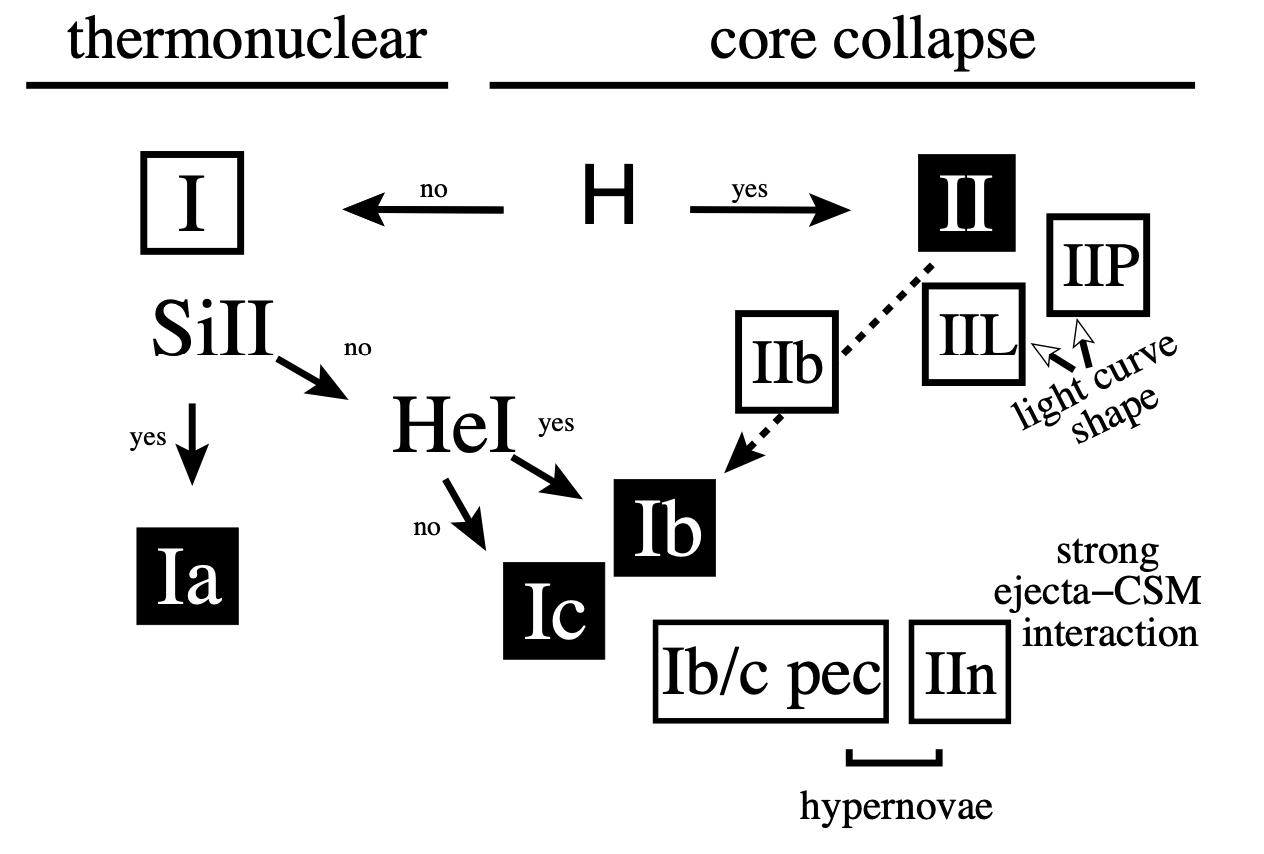
\includegraphics[width=0.7\linewidth]{figures/supernova_class.png }
        \caption{Supernova Classification Scheme (Adapted from  \textcite{Turatto2003}}
        % ]{Supernova classification. The 
        % classification scheme is based on the presence or absence of hydrogen and 
        % silicon features in the spectra of SNe. Figure from}
        \label{fig:sn-classification}
    \end{figure}
\end{frame}

\begin{frame}{DESI}
    \begin{itemize}
        \item Located at Kitt Peak National Observatory, Az
        \item Capable of resolving the [O II] $\lambda \lambda3726,3729$ doublet \parencite{Guy2023}
        \item Bright Galaxy Survey (BGS): $z<0.5$, $\sim10^5$ observed SNe! \parencite{desicollaboration2016, hahn2022}
    \end{itemize}
% The DESI survey focuses on four classes of targets: 14 million bright galaxies\footnote{The BGS contains galaxies with $r$-band magnitudes above 19.5.} in a Bright Galaxy Survey (BGS) at redshifts $z<0.5$; 8 million luminous red galaxies (LRGs) at redshifts $0.4<z<1.2$; 17 million emission line galaxies (ELGs) at $0.6<z<1.6$; and 3 million quasi-stellar objects (QSOs) between $0.9<z<4$. In this work, we will focus on the Bright Galaxy Survey, which is observing host galaxies with a median redshift of $z\approx0.2$ \parencite{desicollaboration2016, hahn2022}.
% DESI began its main survey in May 2021. Over the five-year span of observations, DESI will inevitably observe host galaxies with active SNe, leading to 
% contaminated spectra. The BGS may contain as many as $\sim10^5$ serendipitously observed supernova 
% \parencite{desicollaboration2016}. An example of a supernova observed in a BGS host by DESI and with an independent spectroscopic classification is shown in 
% The presence of transients in DESI spectra is a contaminant for the survey's dark energy program, since the transient can cause a catastrophic failure in the redshift fit, as shown in Figure~\ref{fig:desi_supernova_fail}. Thus it is useful to identify these contaminants whenever possible. Moreover, the serendipitous observation of supernovae is inherently useful since the spectroscopy provides an opportunity to classify {\sl most} types of supernovae without requiring additional follow-up. Both of these factors motivate this study.
\end{frame}

\begin{frame}{DESI Spectra SNe Classification}
    \begin{figure}[t]
        \centering
        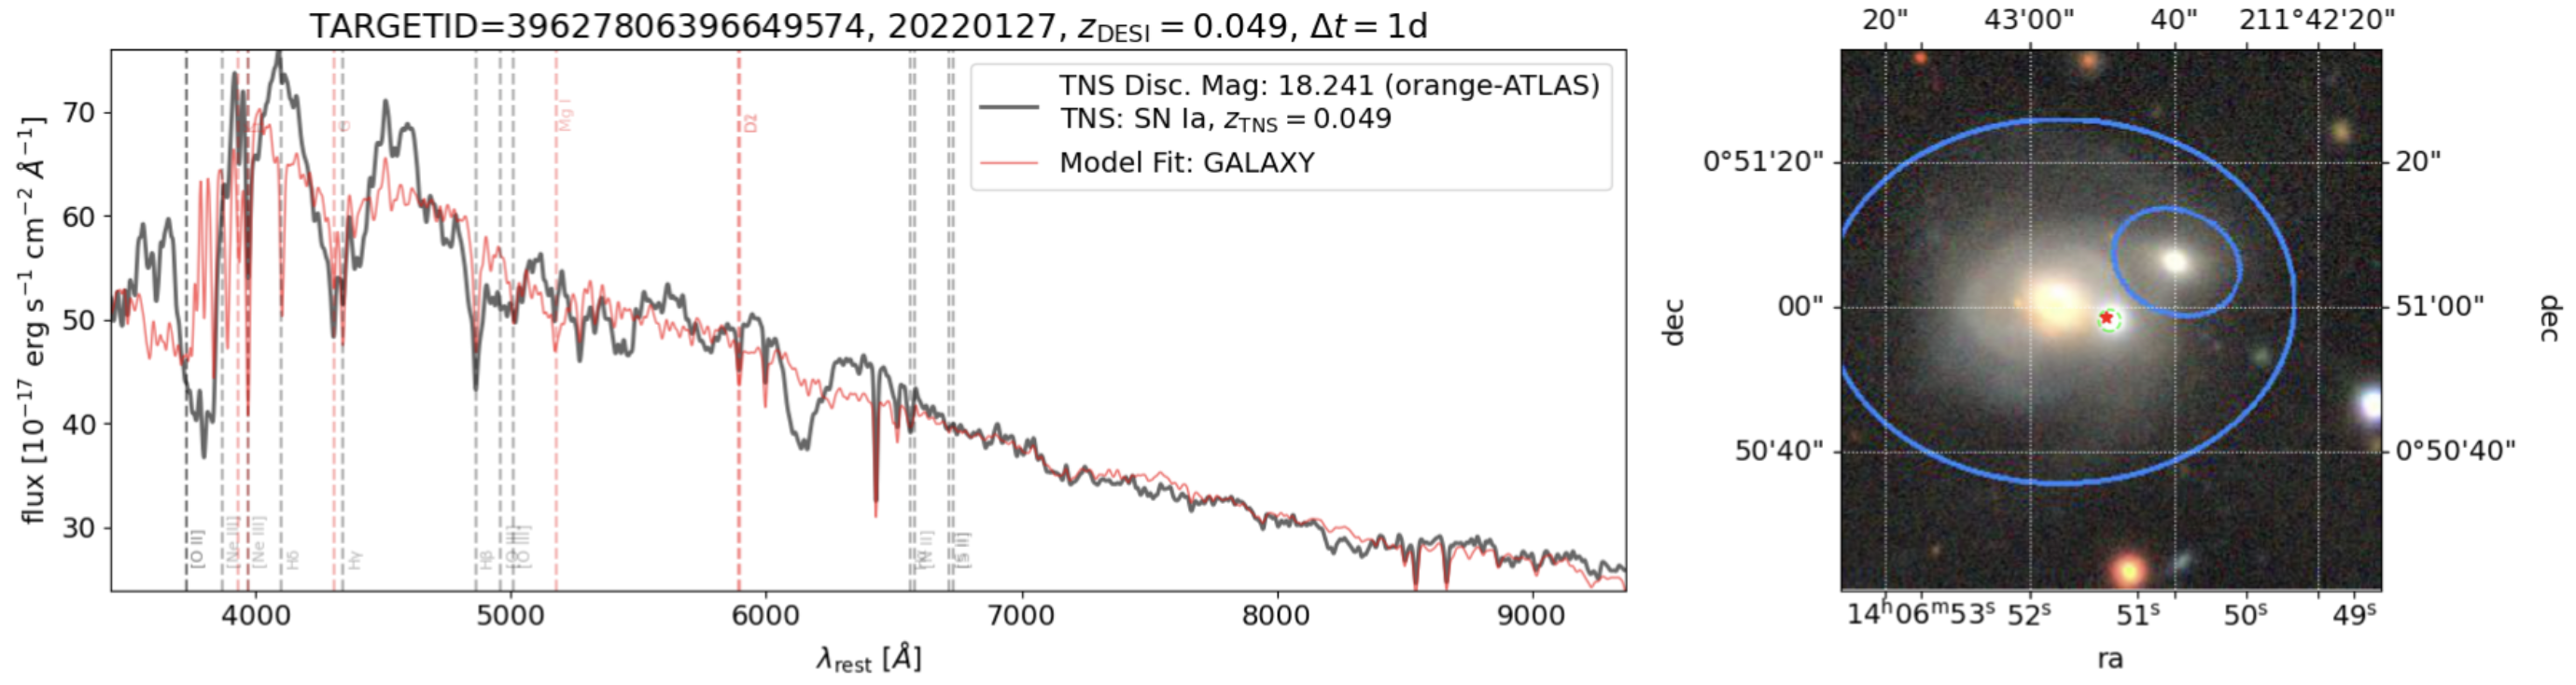
\includegraphics[width=\textwidth]{figures/desi_figures/SNe_Detection.png}
        \caption{DESI Spectra of Publicly Classified SNe Type Ia}
        % captured by DESI]{DESI host galaxy spectrum contaminated by a Type Ia supernova (January 2022). The right panel shows the image of the host galaxy, with the red star indicating the position of the DESI fiber. Independent spectroscopic follow-up reported to the TNS public database confirmed this is an SN Ia.}
        \label{fig:desi_supernova}
%     \end{figure}
% \end{frame}
% \begin{frame}
%     \begin{figure}[t!]
%         \centering
        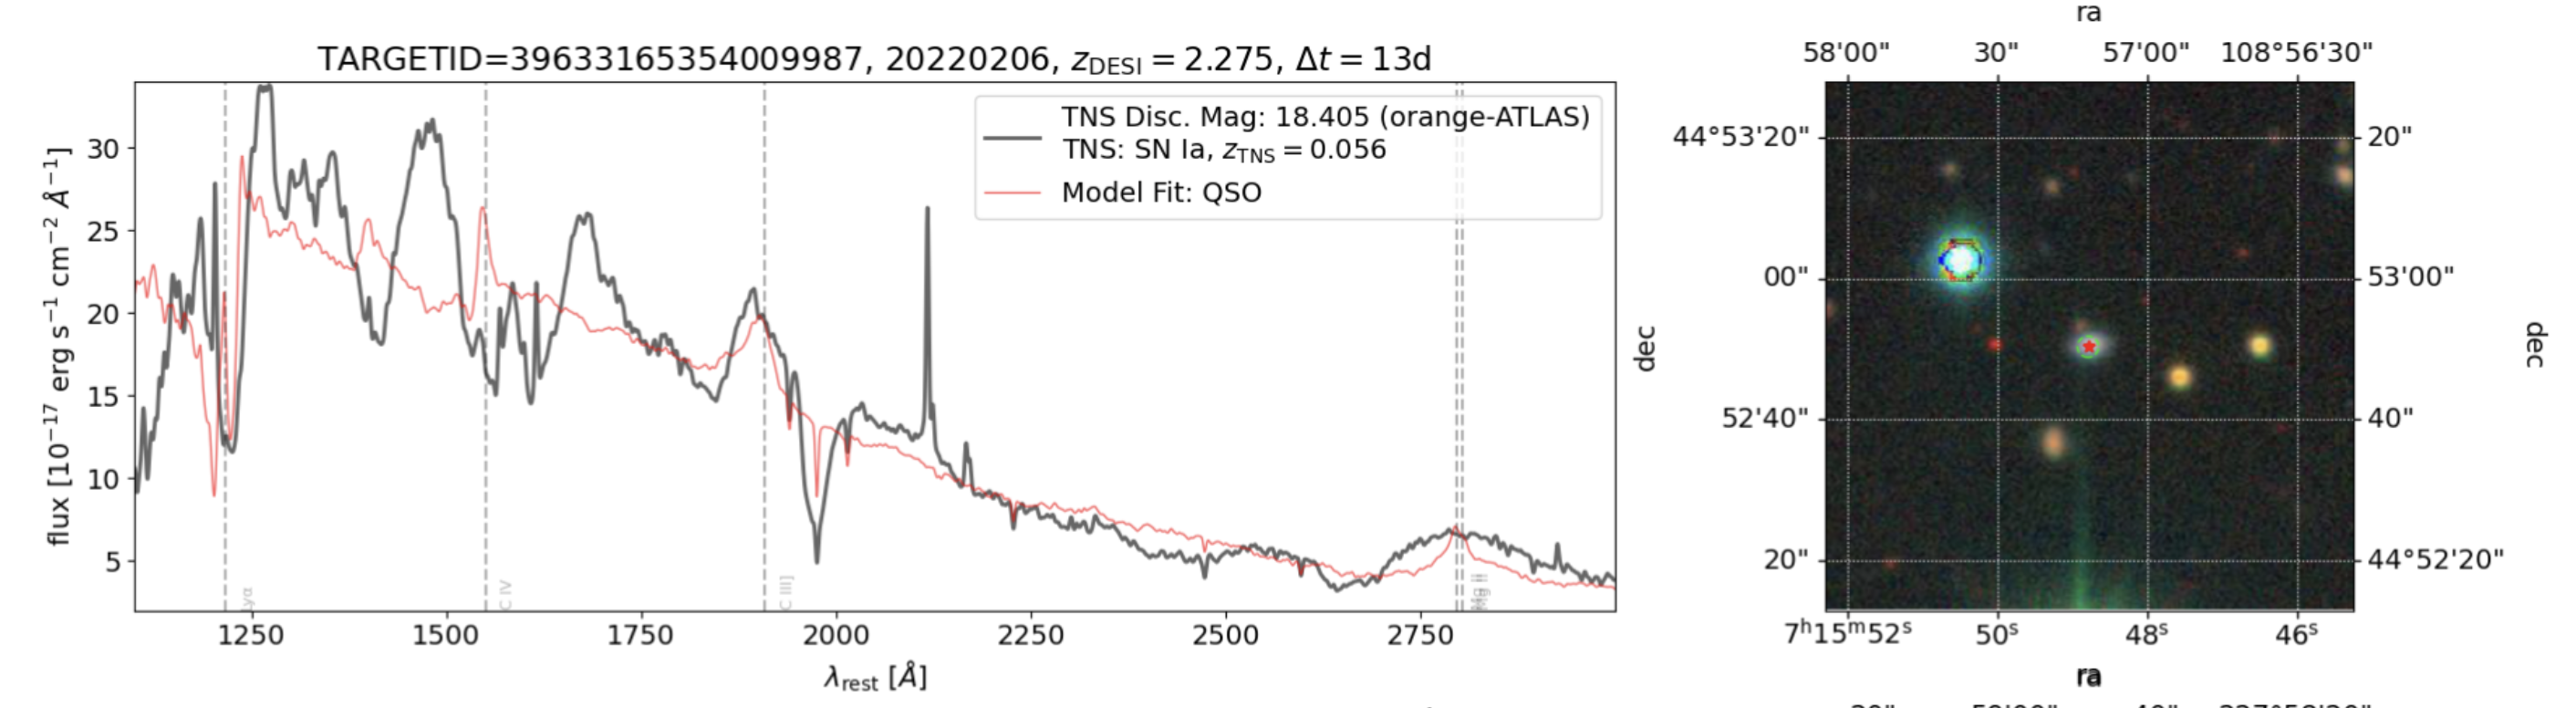
\includegraphics[width=\textwidth]{figures/desi_figures/SNe_detection_desifail.png}
        \caption{DESI Spectra of Publicly Classified SNe Type Ia -- Bad Redshift Fit}
        % Influencing DESI Redshift Fit]{DESI host galaxy spectrum contaminated by a Type Ia supernova (February 2022). The right panel shows the image of the host galaxy, with the red star indicating the position of the DESI fiber. Independent spectroscopic follow-up reported to the TNS public database confirmed this is an SN Ia. Note the extremely poor redshift fit provided by the DESI pipeline.}
        \label{fig:desi_supernova_fail}
    \end{figure}
\end{frame}


\begin{frame}{SNe Template}
    \begin{figure}[t]
        % \centering
        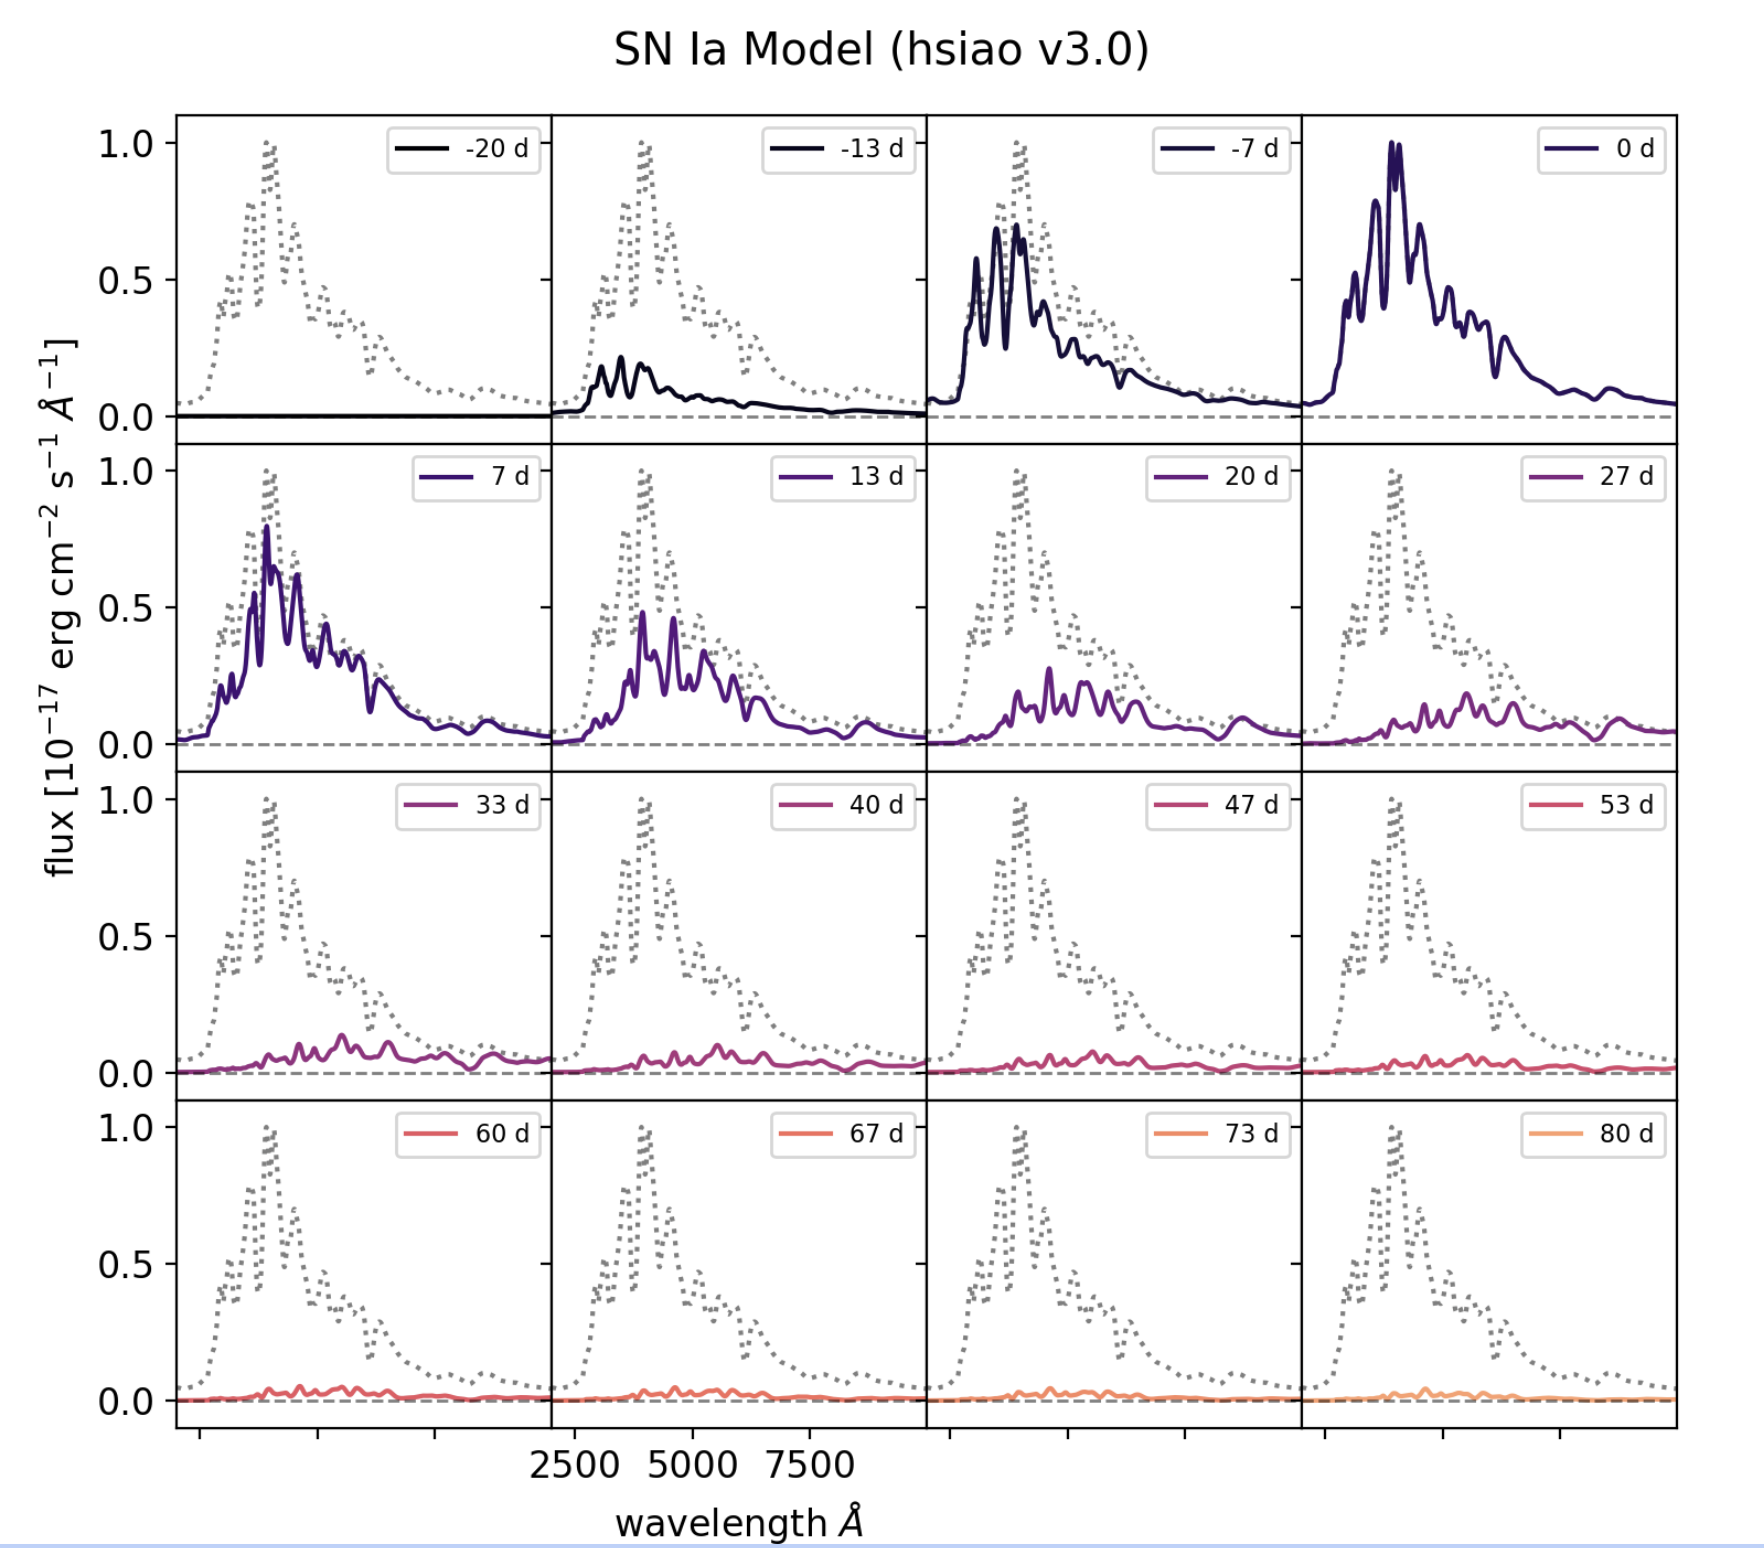
\includegraphics[width=.6\textwidth]{figures/desi_figures/snia_templates.png}
        \caption{Spectral Template of SN Ia SNe (-20$\to$ +80 days after peak) Adapted from \textcite{DESIpresentation}}
        % ]{Spectral model of a SN Ia shown over the course of its evolution, from 20 days before peak brightness to 80 days after. .}
        \label{fig:sne_template}
    \end{figure}
\end{frame}

\begin{frame}{DL in DESI Transient Analysis}
\begin{itemize}
    \item 1D CNN \parencite{wasserman2021}
    \item 2D CNN \parencite{Sepeku2022}
\end{itemize}
Problem: High precision, Low recall
\end{frame}


\begin{comment}
\begin{frame}
    \frametitle{Deep Learning in Medicine}
    \begin{itemize}
        \item<1-> Increase in demand for doctors time \cite{Zhang2020}
        \item<2-> Years of training required to interpret images, yet still inaccuracies occur 
        \item<3-> Helps identify rare diagnosis
    \end{itemize}
\end{frame}
\begin{frame}
    \begin{itemize}
        \item<1-> Small amount of legally available data (HIPAA) 
        \item<2-> Even smaller amount of labeled data (both for classification and segmentation tasks)
        \item<3-> Limited computational resources
        \item<4-> Fear of `black box' solutions
        \item<5-> Solution? Foundational models!
    \end{itemize}
\end{frame}
%%%%%%%%%%%%%%%%%%%%%%%%%%%%%%%%%%%%%%%%%%%%%%%%%%%%%%%%%%%%%%%%%%%%%%%%
\begin{frame}
    \frametitle{Foundational Models}
    \begin{columns}
    \column{0.5\textwidth}
    \begin{figure}
        \centering
        
\includegraphics[width=\linewidth]{figures/blackbox.jpeg}
        \caption{\cite{he2015ResNet}}
    \end{figure}
    \column{0.5\textwidth}
    \begin{figure}
        \centering
        
\includegraphics[width=\linewidth]{figures/blackbox.jpeg}
        \caption{\cite{Liu2021V2}}
    \end{figure}
    \end{columns}
        \begin{figure}
        \centering
        
\includegraphics[width=\linewidth]{figures/blackbox.jpeg}
        \caption{\cite{Long2014}}
    \end{figure}
\end{frame}
%%%%%%%%%%%%%%%%%%%%%%%%%%%%%%%%%%%%%%%%%%%%%%%%%%%%%%%%%%%%%%%%%%%%%%%%
\begin{frame}
    \frametitle{This Is anotherFrame}
    \resizebox{\linewidth}{!}{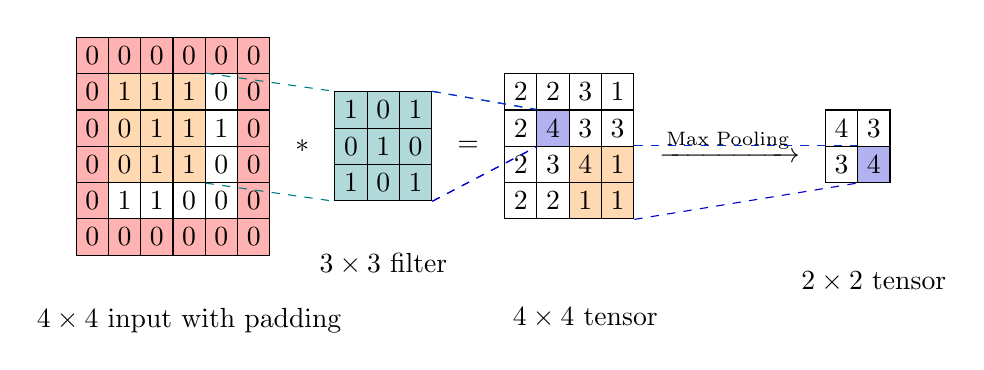
\begin{tikzpicture}[
    2d-arr/.style={matrix of nodes, row sep=-\pgflinewidth, column sep=-\pgflinewidth, nodes={draw}}
  ]

  \matrix (mtr) [2d-arr] {
  |[fill=red!30]| 0  & |[fill=red!30]| 0  & |[fill=red!30]| 0  & |[fill=red!30]| 0  & |[fill=red!30]| 0  & |[fill=red!30]| 0 \\
  |[fill=red!30]| 0  & |[fill=orange!30]| 1 & |[fill=orange!30]| 1 & |[fill=orange!30]| 1 &  0 & |[fill=red!30]| 0 \\
  |[fill=red!30]| 0  & |[fill=orange!30]| 0 & |[fill=orange!30]| 1 & |[fill=orange!30]| 1 &  1 & |[fill=red!30]| 0 \\
  |[fill=red!30]| 0  & |[fill=orange!30]| 0 & |[fill=orange!30]| 1 & |[fill=orange!30]| 1 & 0 & |[fill=red!30]| 0 \\
  |[fill=red!30]| 0  & 1 & 1 & 0 & 0 & |[fill=red!30]| 0 \\
  |[fill=red!30]| 0  & |[fill=red!30]| 0  & |[fill=red!30]| 0  & |[fill=red!30]| 0  & |[fill=red!30]| 0  & |[fill=red!30]| 0 \\
  };

  \node[below=of mtr-5-4] {$4\times4$ input with padding};

  \node[right=0.2em of mtr] (str) {$*$};

  \matrix (K) [2d-arr, right=0.2em of str, nodes={draw, fill=teal!30}] {
    1 & 0 &1\\
    0 & 1 &0\\
    1 & 0 & 1\\
  };
  \node[below=of K-2-2] {$3\times3$ filter};

  \node[right=0.2em of K] (eq) {$=$};

  \matrix (ret) [2d-arr, right=0.2em of eq] {
  2 & 2 & 3 &  1\\
  2 & |[fill=blue!80!black!30]| 4 & 3 & 3\\
  2 & 3 & |[fill=orange!30]| 4 & |[fill=orange!30]| 1 \\
  2 & 2 & |[fill=orange!30]| 1 & |[fill=orange!30]| 1 \\
  };
  \node[below=of ret-4-3] {$4\times4$ tensor};

  \node[right=0.2em of ret] (ra) {$\xrightarrow[]{\text{Max Pooling}}$};

\matrix (pool) [2d-arr, right=0.2em of ra] {
  4 & 3 \\
  3 & |[fill=blue!80!black!30]| 4 \\
  };
  \node[below=of pool-2-2] {$2\times2$ tensor};

  \draw[dashed, teal] (mtr-2-4.north east) -- (K-1-1.north west);
  \draw[dashed, teal] (mtr-4-4.south east) -- (K-3-1.south west);

  \draw[dashed, blue!80!green] (K-1-3.north east) -- (ret-2-2.north west);
  \draw[dashed, blue!80!black] (K-3-3.south east) -- (ret-2-2.south west);

  \draw[dashed, blue!80!green] (K-1-3.north east) -- (ret-2-2.north west);
  \draw[dashed, blue!80!black] (K-3-3.south east) -- (ret-2-2.south west);

\draw[dashed, blue!80!green] (ret-3-4.north east) -- (pool-2-2.north west);
  \draw[dashed, blue!80!black] (ret-4-4.south east) -- (pool-2-2.south west);

\end{tikzpicture}
}
\end{frame}
%%%%%%%%%%%%%%%%%%%%%%%%%%%%%%%%%%%%%%%%%%%%%%%%%%%%%%%%%%%%%%%%%%%%%%%%
\begin{frame}
    \frametitle{ThisIsaFrame}
    \resizebox{\linewidth}{!}{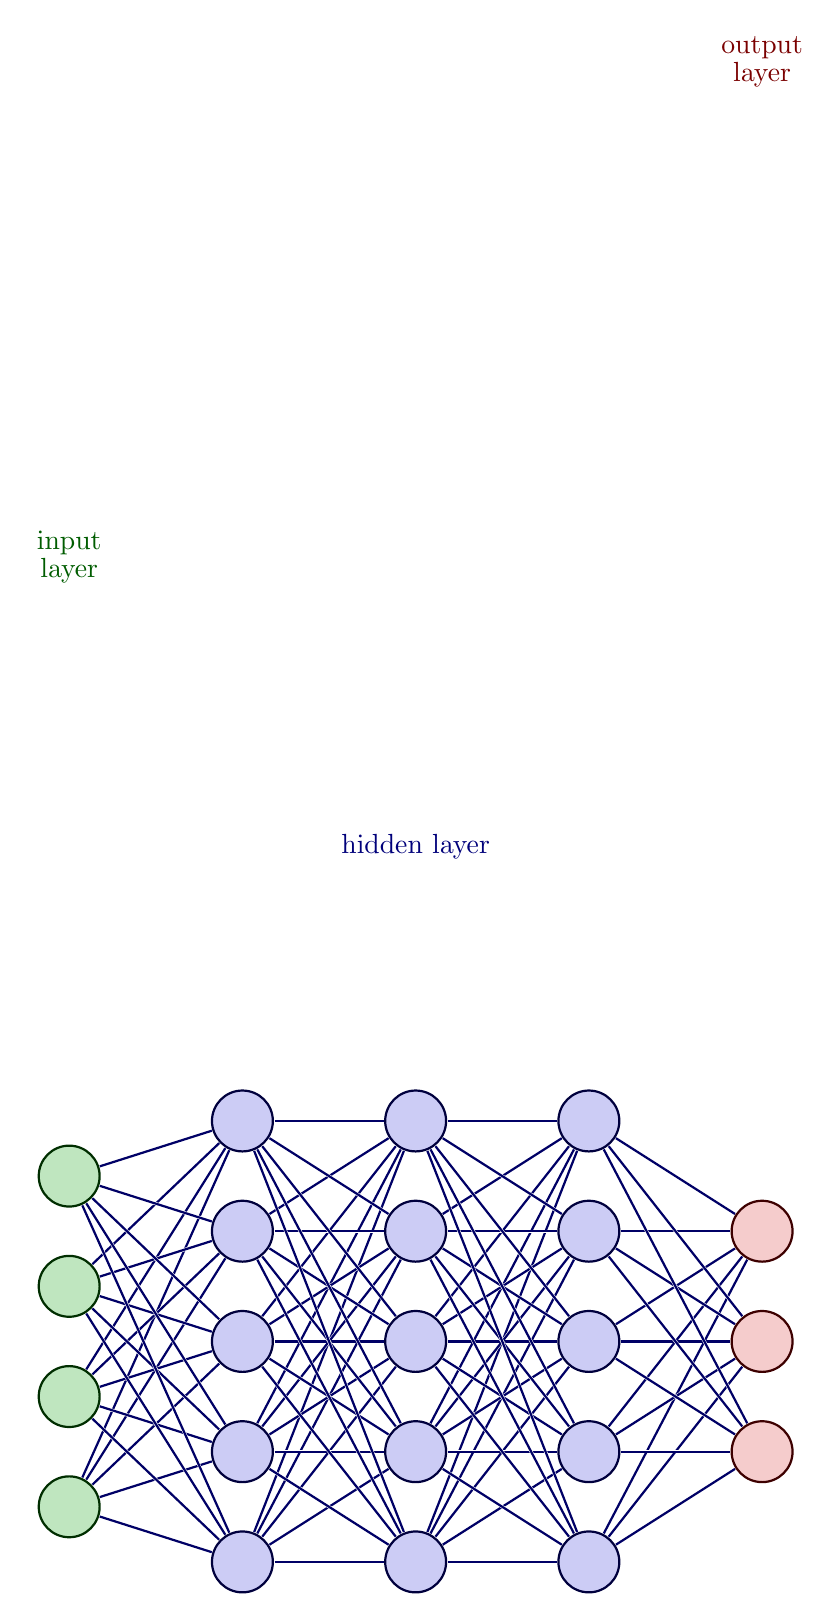
\begin{tikzpicture}[x=2.2cm,y=1.4cm]
  \message{^^JNeural network without text}
  \readlist\Nnod{4,5,5,5,3} % array of number of nodes per layer
  
  \message{^^J  Layer}
  \foreachitem \N \in \Nnod{ % loop over layers
    \def\lay{\Ncnt} % alias of index of current layer
    \pgfmathsetmacro\prev{int(\Ncnt-1)} % number of previous layer
    \message{\lay,}
    \foreach \i [evaluate={\y=\N/2-\i; \x=\lay; \n=\nstyle;}] in {1,...,\N}{ % loop over nodes
      
      % NODES
      \node[node \n] (N\lay-\i) at (\x,\y) {};
      
      % CONNECTIONS
      \ifnum\lay>1 % connect to previous layer
        \foreach \j in {1,...,\Nnod[\prev]}{ % loop over nodes in previous layer
          \draw[connect,white,line width=1.2] (N\prev-\j) -- (N\lay-\i);
          \draw[connect] (N\prev-\j) -- (N\lay-\i);
          %\draw[connect] (N\prev-\j.0) -- (N\lay-\i.180); % connect to left
        }
      \fi % else: nothing to connect first layer
      
    }
  }
  
  % LABELS
  \node[above=5,align=center,mygreen!60!black] at (N1-1.90) {input\\[-0.2em]layer};
  \node[above=2,align=center,myblue!60!black] at (N3-1.90) {hidden layer};
  \node[above=10,align=center,myred!60!black] at (N\Nnodlen-1.90) {output\\[-0.2em]layer};
  
\end{tikzpicture}
}
\end{frame}
\end{comment}

%%%%%%%%%%%%%%%%%%%%%%%%%%%%%%%%%%%%%%%%%%%%%%%%%%%%%%%%%%%%%%%%%%%%%%%%

\section{Deep Learning Techniques}
%%%%%%%%%%%%%%%%%%%%%%%%%%%%%%%%%%%%%%%%%%%%%%%%%%%%%%%%%%%%%%%%%%%%%%%%
\begin{frame}{Multi-Layer Perceptron}
    \begin{figure}[t]
        \centering
        \resizebox{.6\linewidth}{!}{\input{tikz/MLP}}
        \caption{Multi-Layered Perceptron (adapted from \textcite{neutelings2021_nn})}
        % ]{A simple MLP with an input dimension of 4 (green nodes), three hidden layers (blue nodes), and an output dimension of 3 (red nodes). Each node is connected to every node in the previous and next layer. The lines represent the weights, and each  node has an associated bias. Figure adapted from 
        \label{fig:MLP}
    \end{figure}
\end{frame}

\begin{frame}{CNN Architecture}
    \begin{figure}[t]
        \centering 
        \resizebox{.6\linewidth}{!}{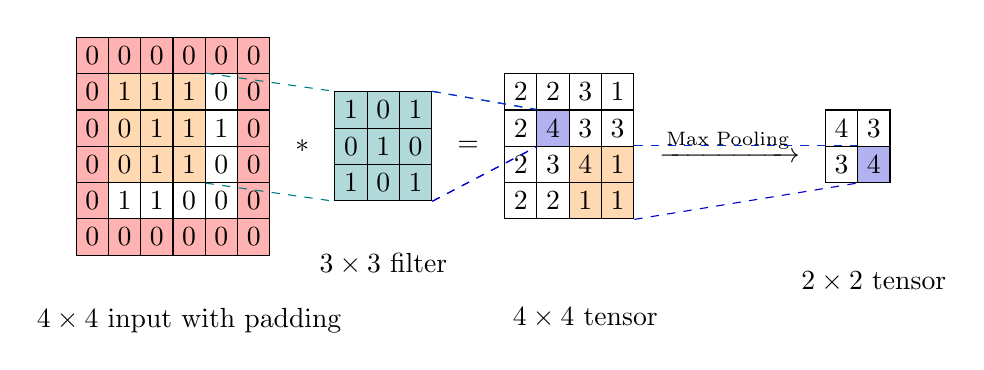
\begin{tikzpicture}[
    2d-arr/.style={matrix of nodes, row sep=-\pgflinewidth, column sep=-\pgflinewidth, nodes={draw}}
  ]

  \matrix (mtr) [2d-arr] {
  |[fill=red!30]| 0  & |[fill=red!30]| 0  & |[fill=red!30]| 0  & |[fill=red!30]| 0  & |[fill=red!30]| 0  & |[fill=red!30]| 0 \\
  |[fill=red!30]| 0  & |[fill=orange!30]| 1 & |[fill=orange!30]| 1 & |[fill=orange!30]| 1 &  0 & |[fill=red!30]| 0 \\
  |[fill=red!30]| 0  & |[fill=orange!30]| 0 & |[fill=orange!30]| 1 & |[fill=orange!30]| 1 &  1 & |[fill=red!30]| 0 \\
  |[fill=red!30]| 0  & |[fill=orange!30]| 0 & |[fill=orange!30]| 1 & |[fill=orange!30]| 1 & 0 & |[fill=red!30]| 0 \\
  |[fill=red!30]| 0  & 1 & 1 & 0 & 0 & |[fill=red!30]| 0 \\
  |[fill=red!30]| 0  & |[fill=red!30]| 0  & |[fill=red!30]| 0  & |[fill=red!30]| 0  & |[fill=red!30]| 0  & |[fill=red!30]| 0 \\
  };

  \node[below=of mtr-5-4] {$4\times4$ input with padding};

  \node[right=0.2em of mtr] (str) {$*$};

  \matrix (K) [2d-arr, right=0.2em of str, nodes={draw, fill=teal!30}] {
    1 & 0 &1\\
    0 & 1 &0\\
    1 & 0 & 1\\
  };
  \node[below=of K-2-2] {$3\times3$ filter};

  \node[right=0.2em of K] (eq) {$=$};

  \matrix (ret) [2d-arr, right=0.2em of eq] {
  2 & 2 & 3 &  1\\
  2 & |[fill=blue!80!black!30]| 4 & 3 & 3\\
  2 & 3 & |[fill=orange!30]| 4 & |[fill=orange!30]| 1 \\
  2 & 2 & |[fill=orange!30]| 1 & |[fill=orange!30]| 1 \\
  };
  \node[below=of ret-4-3] {$4\times4$ tensor};

  \node[right=0.2em of ret] (ra) {$\xrightarrow[]{\text{Max Pooling}}$};

\matrix (pool) [2d-arr, right=0.2em of ra] {
  4 & 3 \\
  3 & |[fill=blue!80!black!30]| 4 \\
  };
  \node[below=of pool-2-2] {$2\times2$ tensor};

  \draw[dashed, teal] (mtr-2-4.north east) -- (K-1-1.north west);
  \draw[dashed, teal] (mtr-4-4.south east) -- (K-3-1.south west);

  \draw[dashed, blue!80!green] (K-1-3.north east) -- (ret-2-2.north west);
  \draw[dashed, blue!80!black] (K-3-3.south east) -- (ret-2-2.south west);

  \draw[dashed, blue!80!green] (K-1-3.north east) -- (ret-2-2.north west);
  \draw[dashed, blue!80!black] (K-3-3.south east) -- (ret-2-2.south west);

\draw[dashed, blue!80!green] (ret-3-4.north east) -- (pool-2-2.north west);
  \draw[dashed, blue!80!black] (ret-4-4.south east) -- (pool-2-2.south west);

\end{tikzpicture}
}
        \caption{CNN Unit ( adapted from \textcite{neutelings2022_conv})}
        \label{fig:convolution}
    % \end{figure}
    % \begin{figure}[t]
    %     \centering
        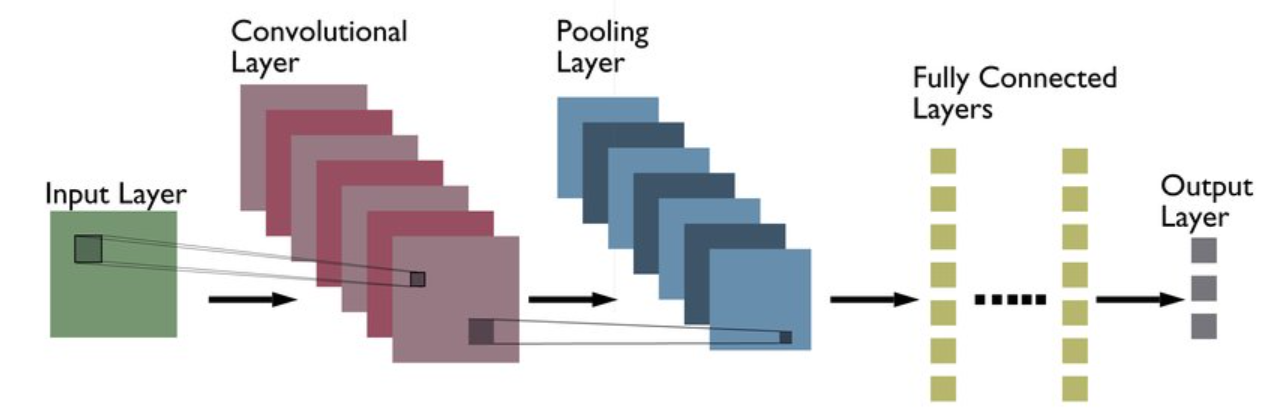
\includegraphics[width=.8\linewidth]{figures/Typical-CNN-architecture.png}
        \caption{Traditional CNN Architecture for Classification (adapted from \cite{kumar2022_cnn})}
        \label{fig:CNN}
    \end{figure}
\end{frame}

\begin{frame}{2D CNN Performance}
    \begin{figure}
        \centering
        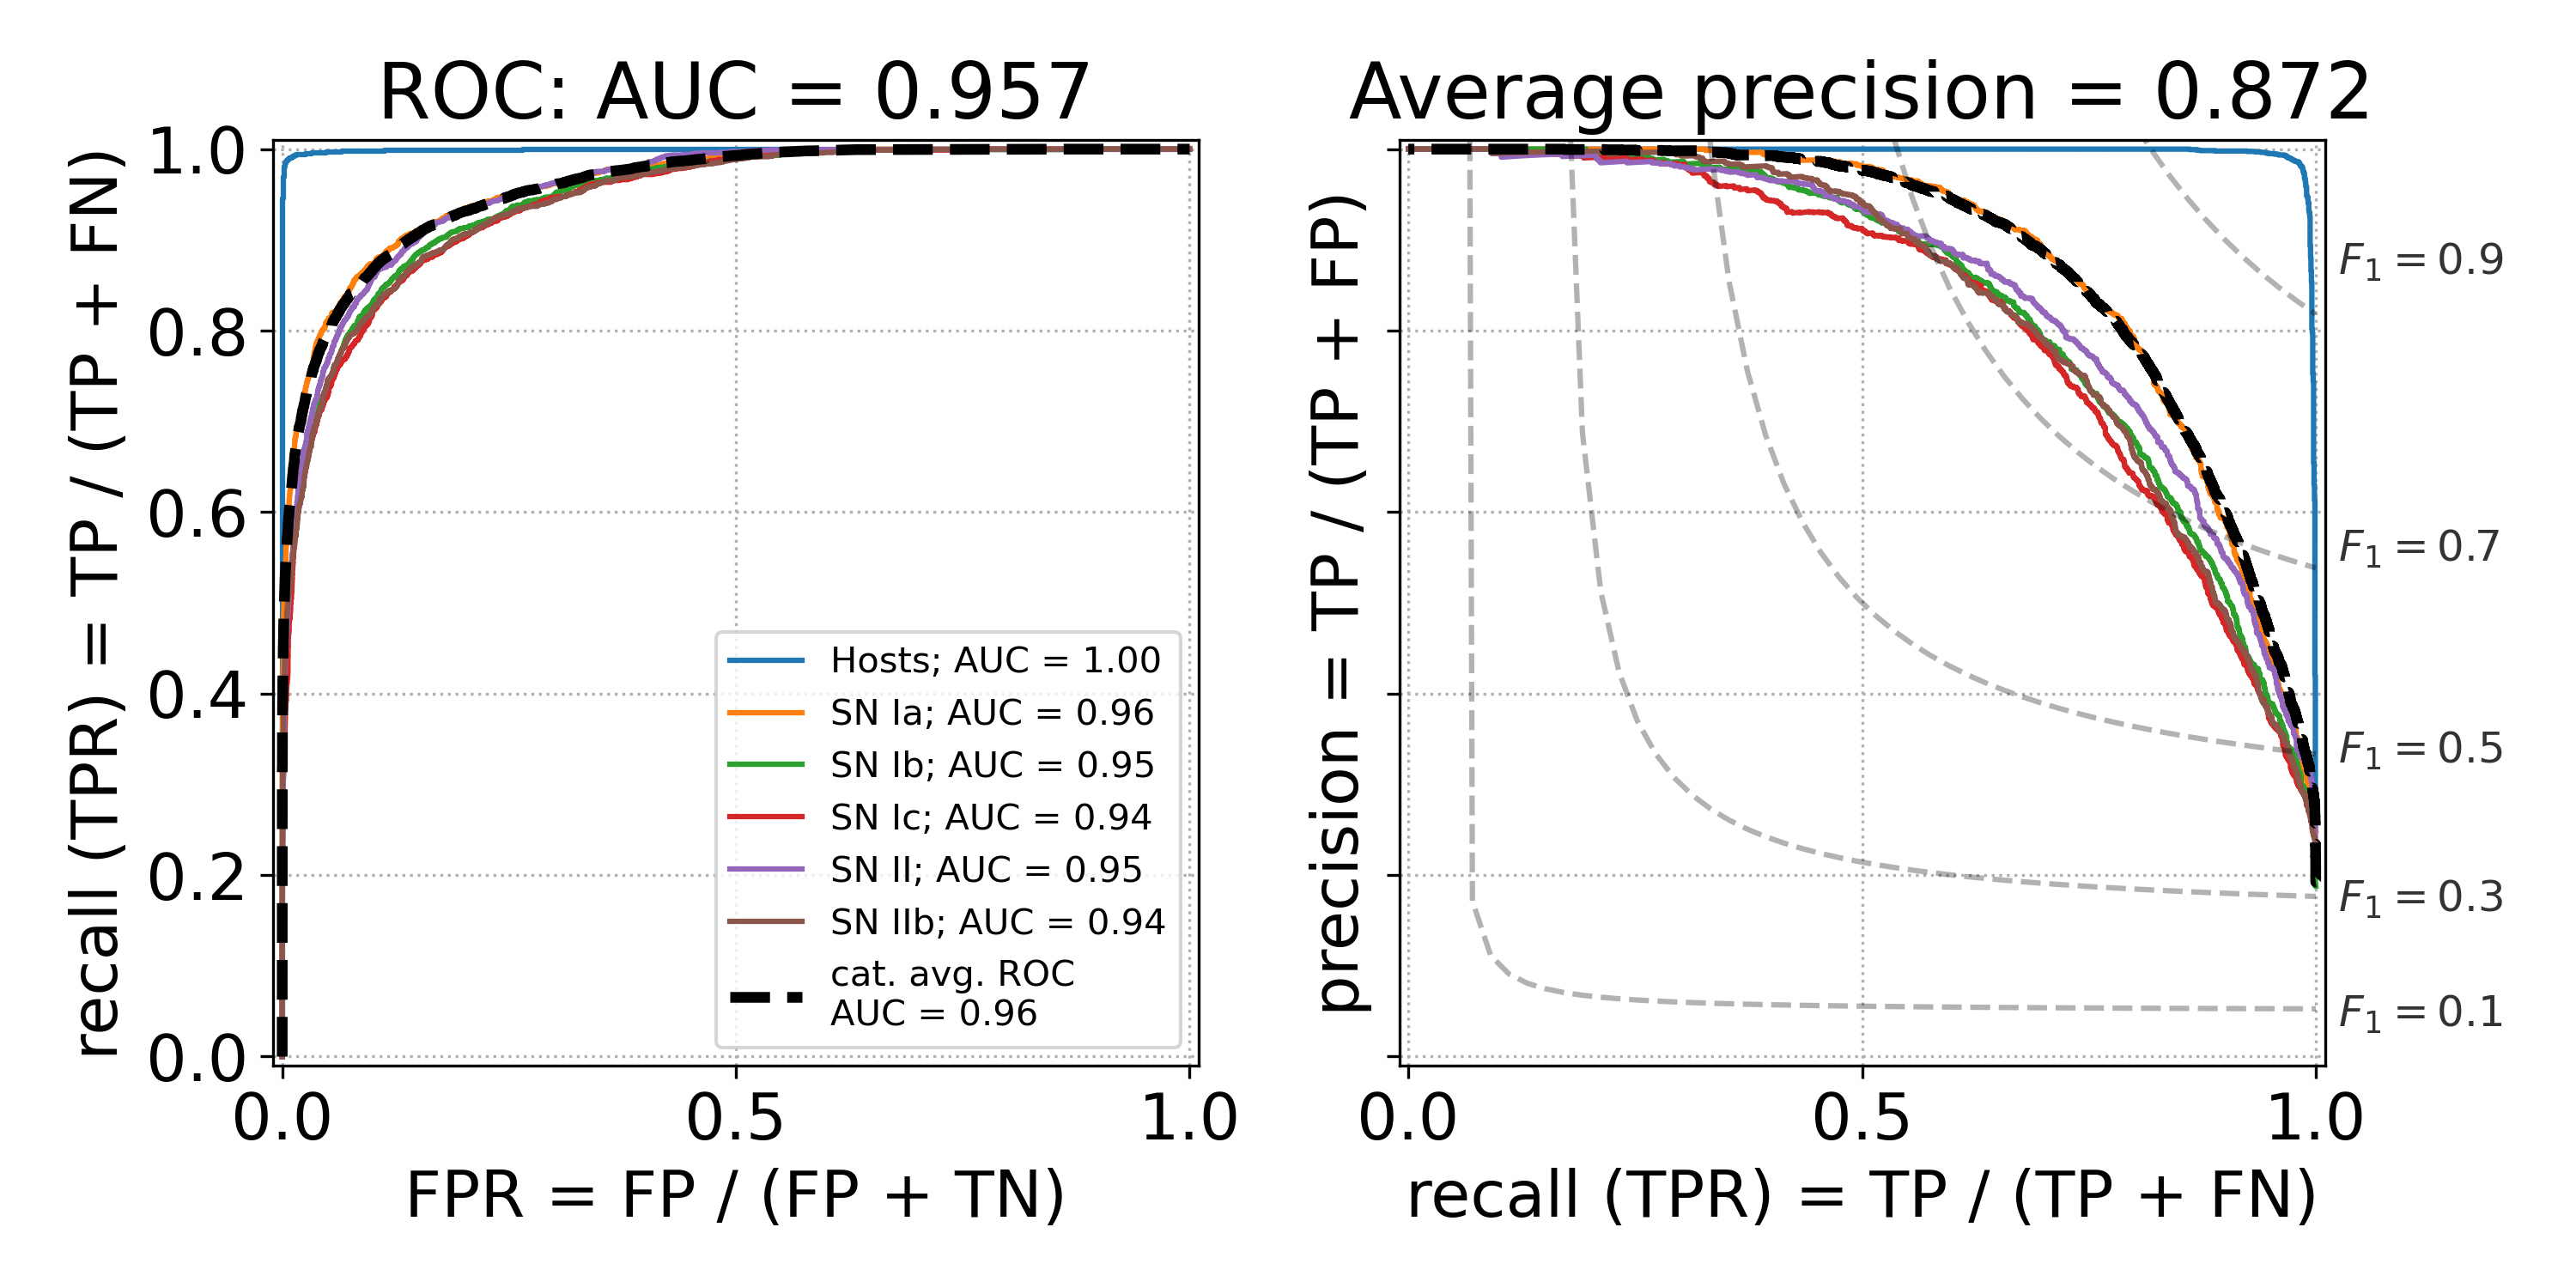
\includegraphics[height=2.8cm]{figures/cnn/cnn_rocfull.png}
        \quad
        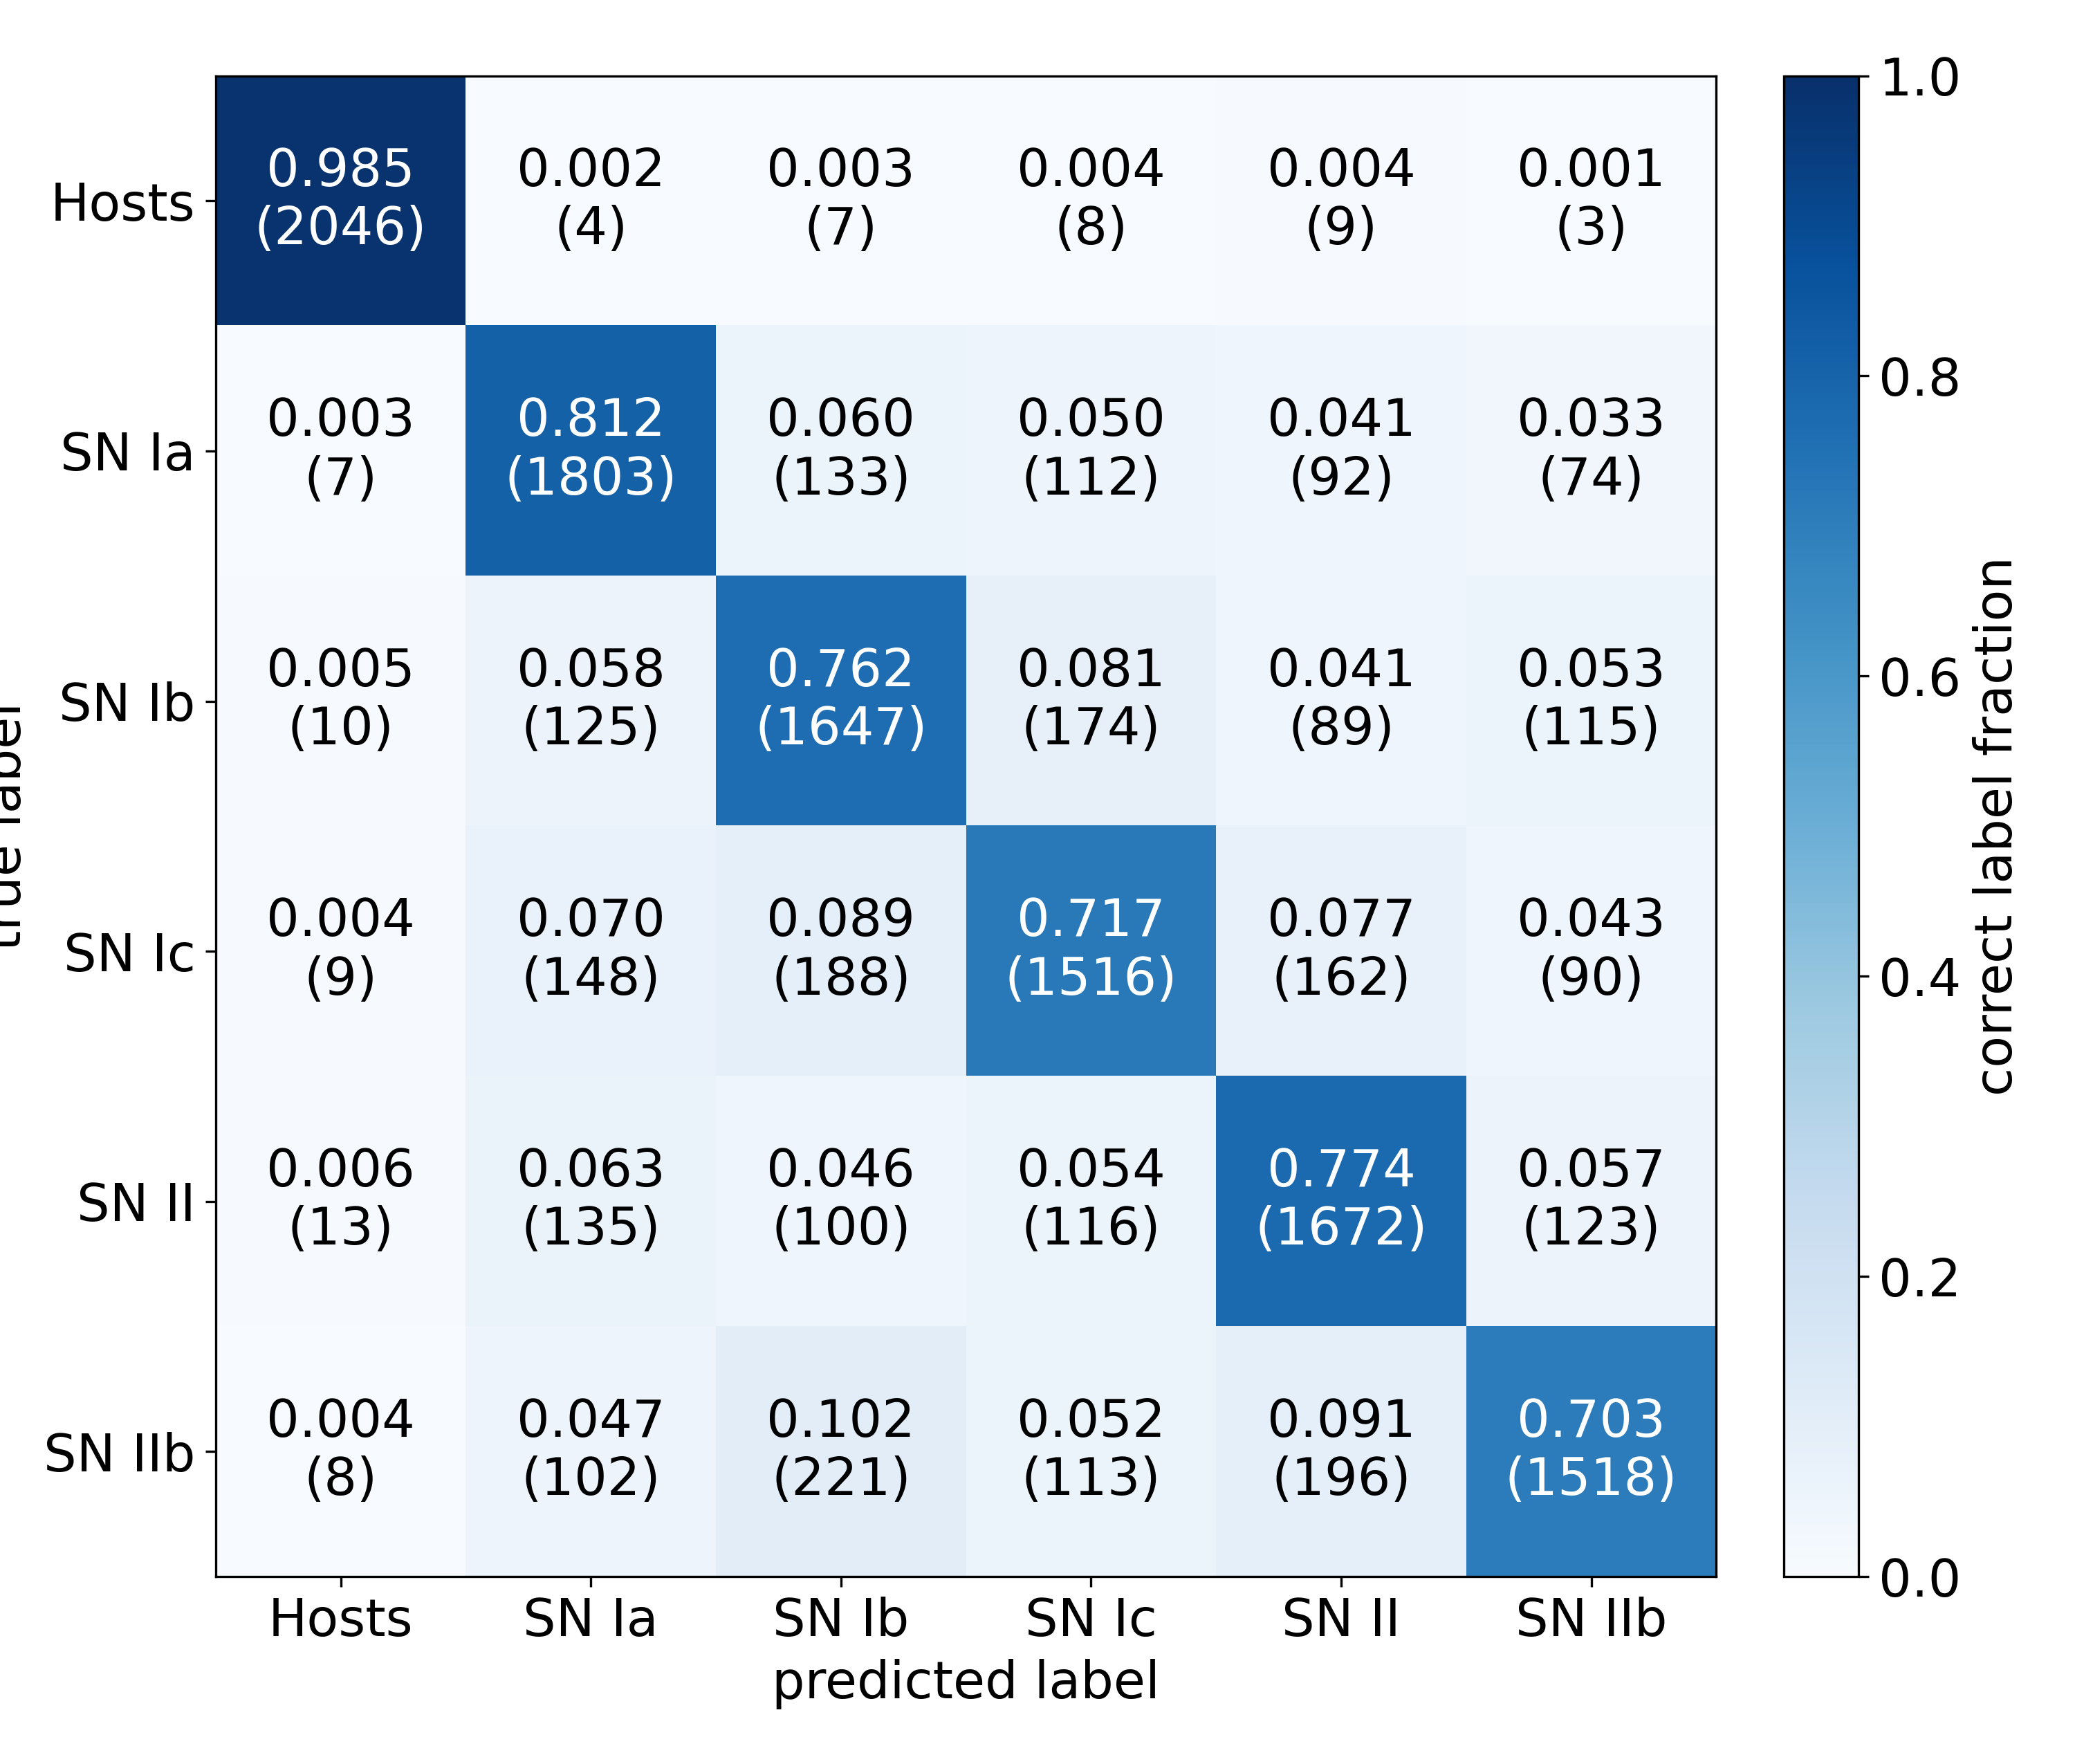
\includegraphics[height=2.8cm]{figures/cnn/cnn_cmfull.png}
        \caption{CNN Classifier}
%     \end{figure}
% \end{frame}

% \begin{frame}
%     \begin{figure}[t!]
%         \centering
        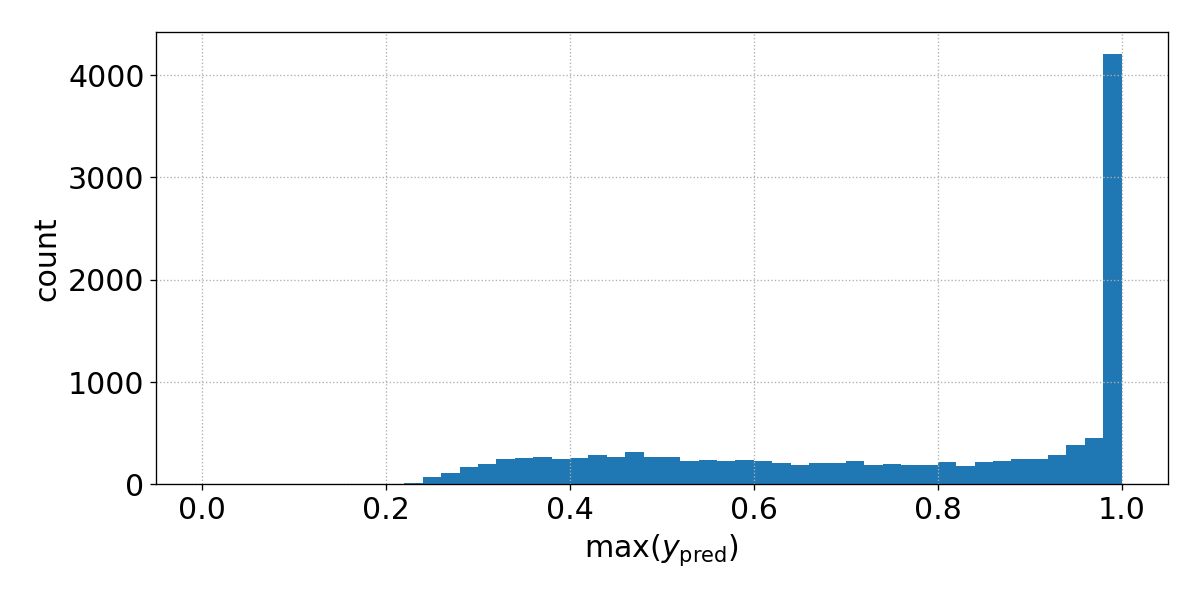
\includegraphics[width=0.5\textwidth]{figures/cnn/cnn_max_ypred.png}
        \caption{CNN's Maximum Output Vector\label{fig:cnn_max}}
    \end{figure}
\end{frame}

\begin{frame}{CNN Cut to Increase Performance}
    \begin{figure}[b]
        \centering
        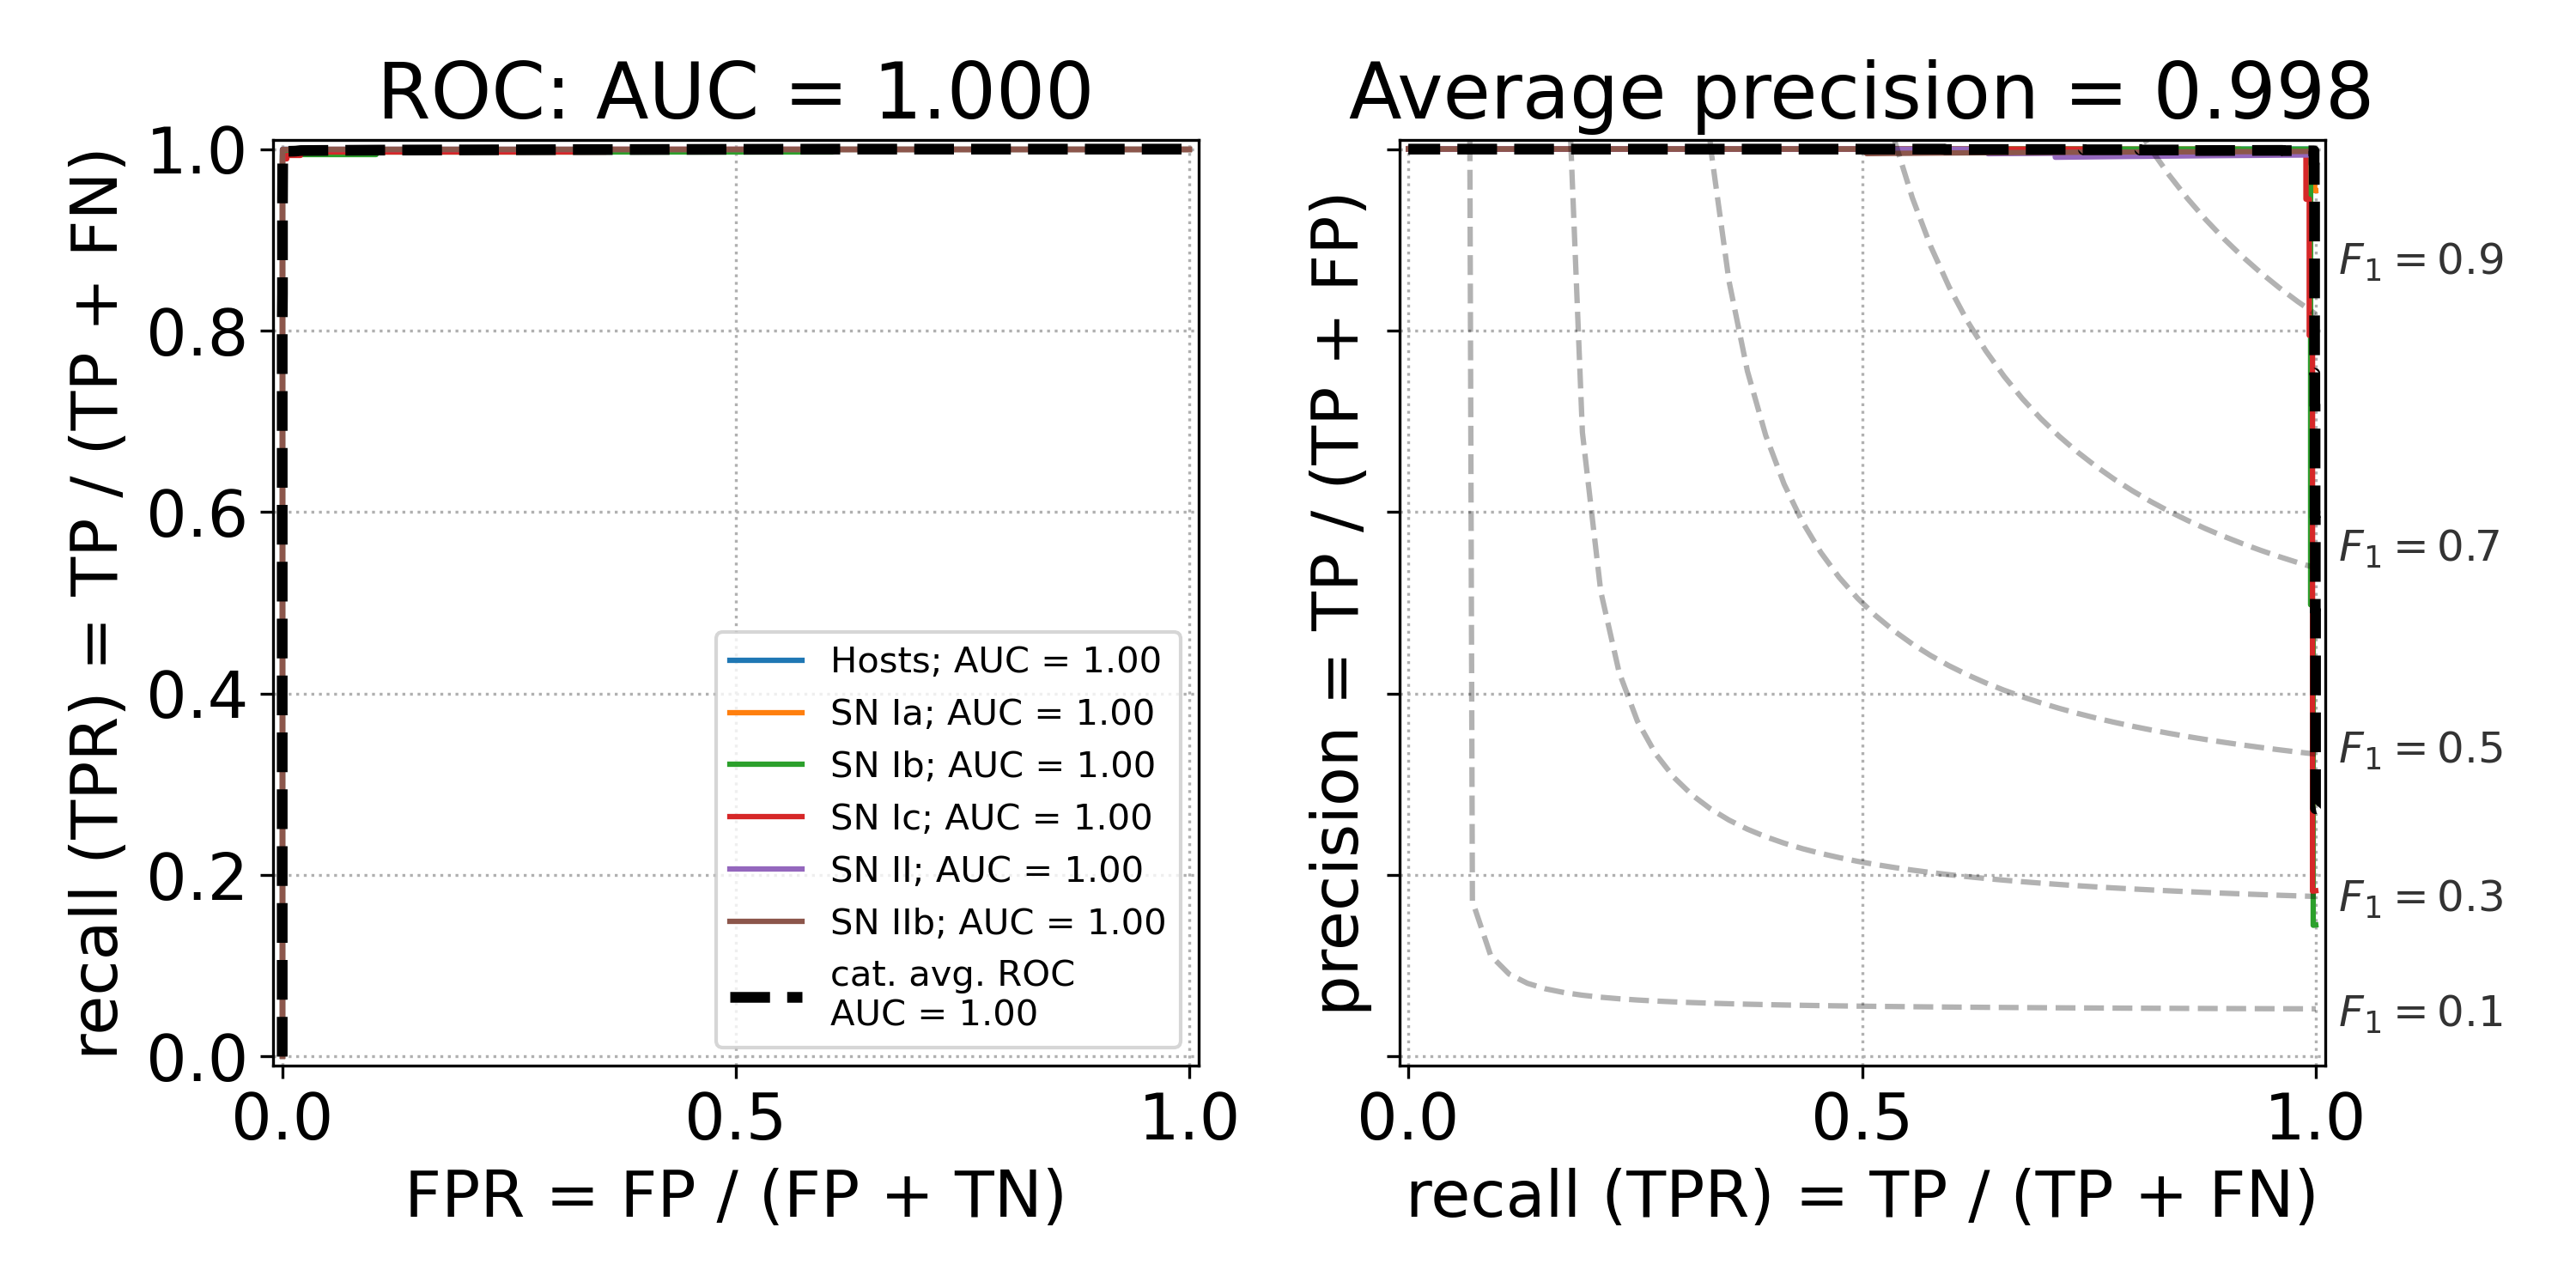
\includegraphics[height=2.6cm]{figures/cnn/cnn_roc99.png}
        \quad
        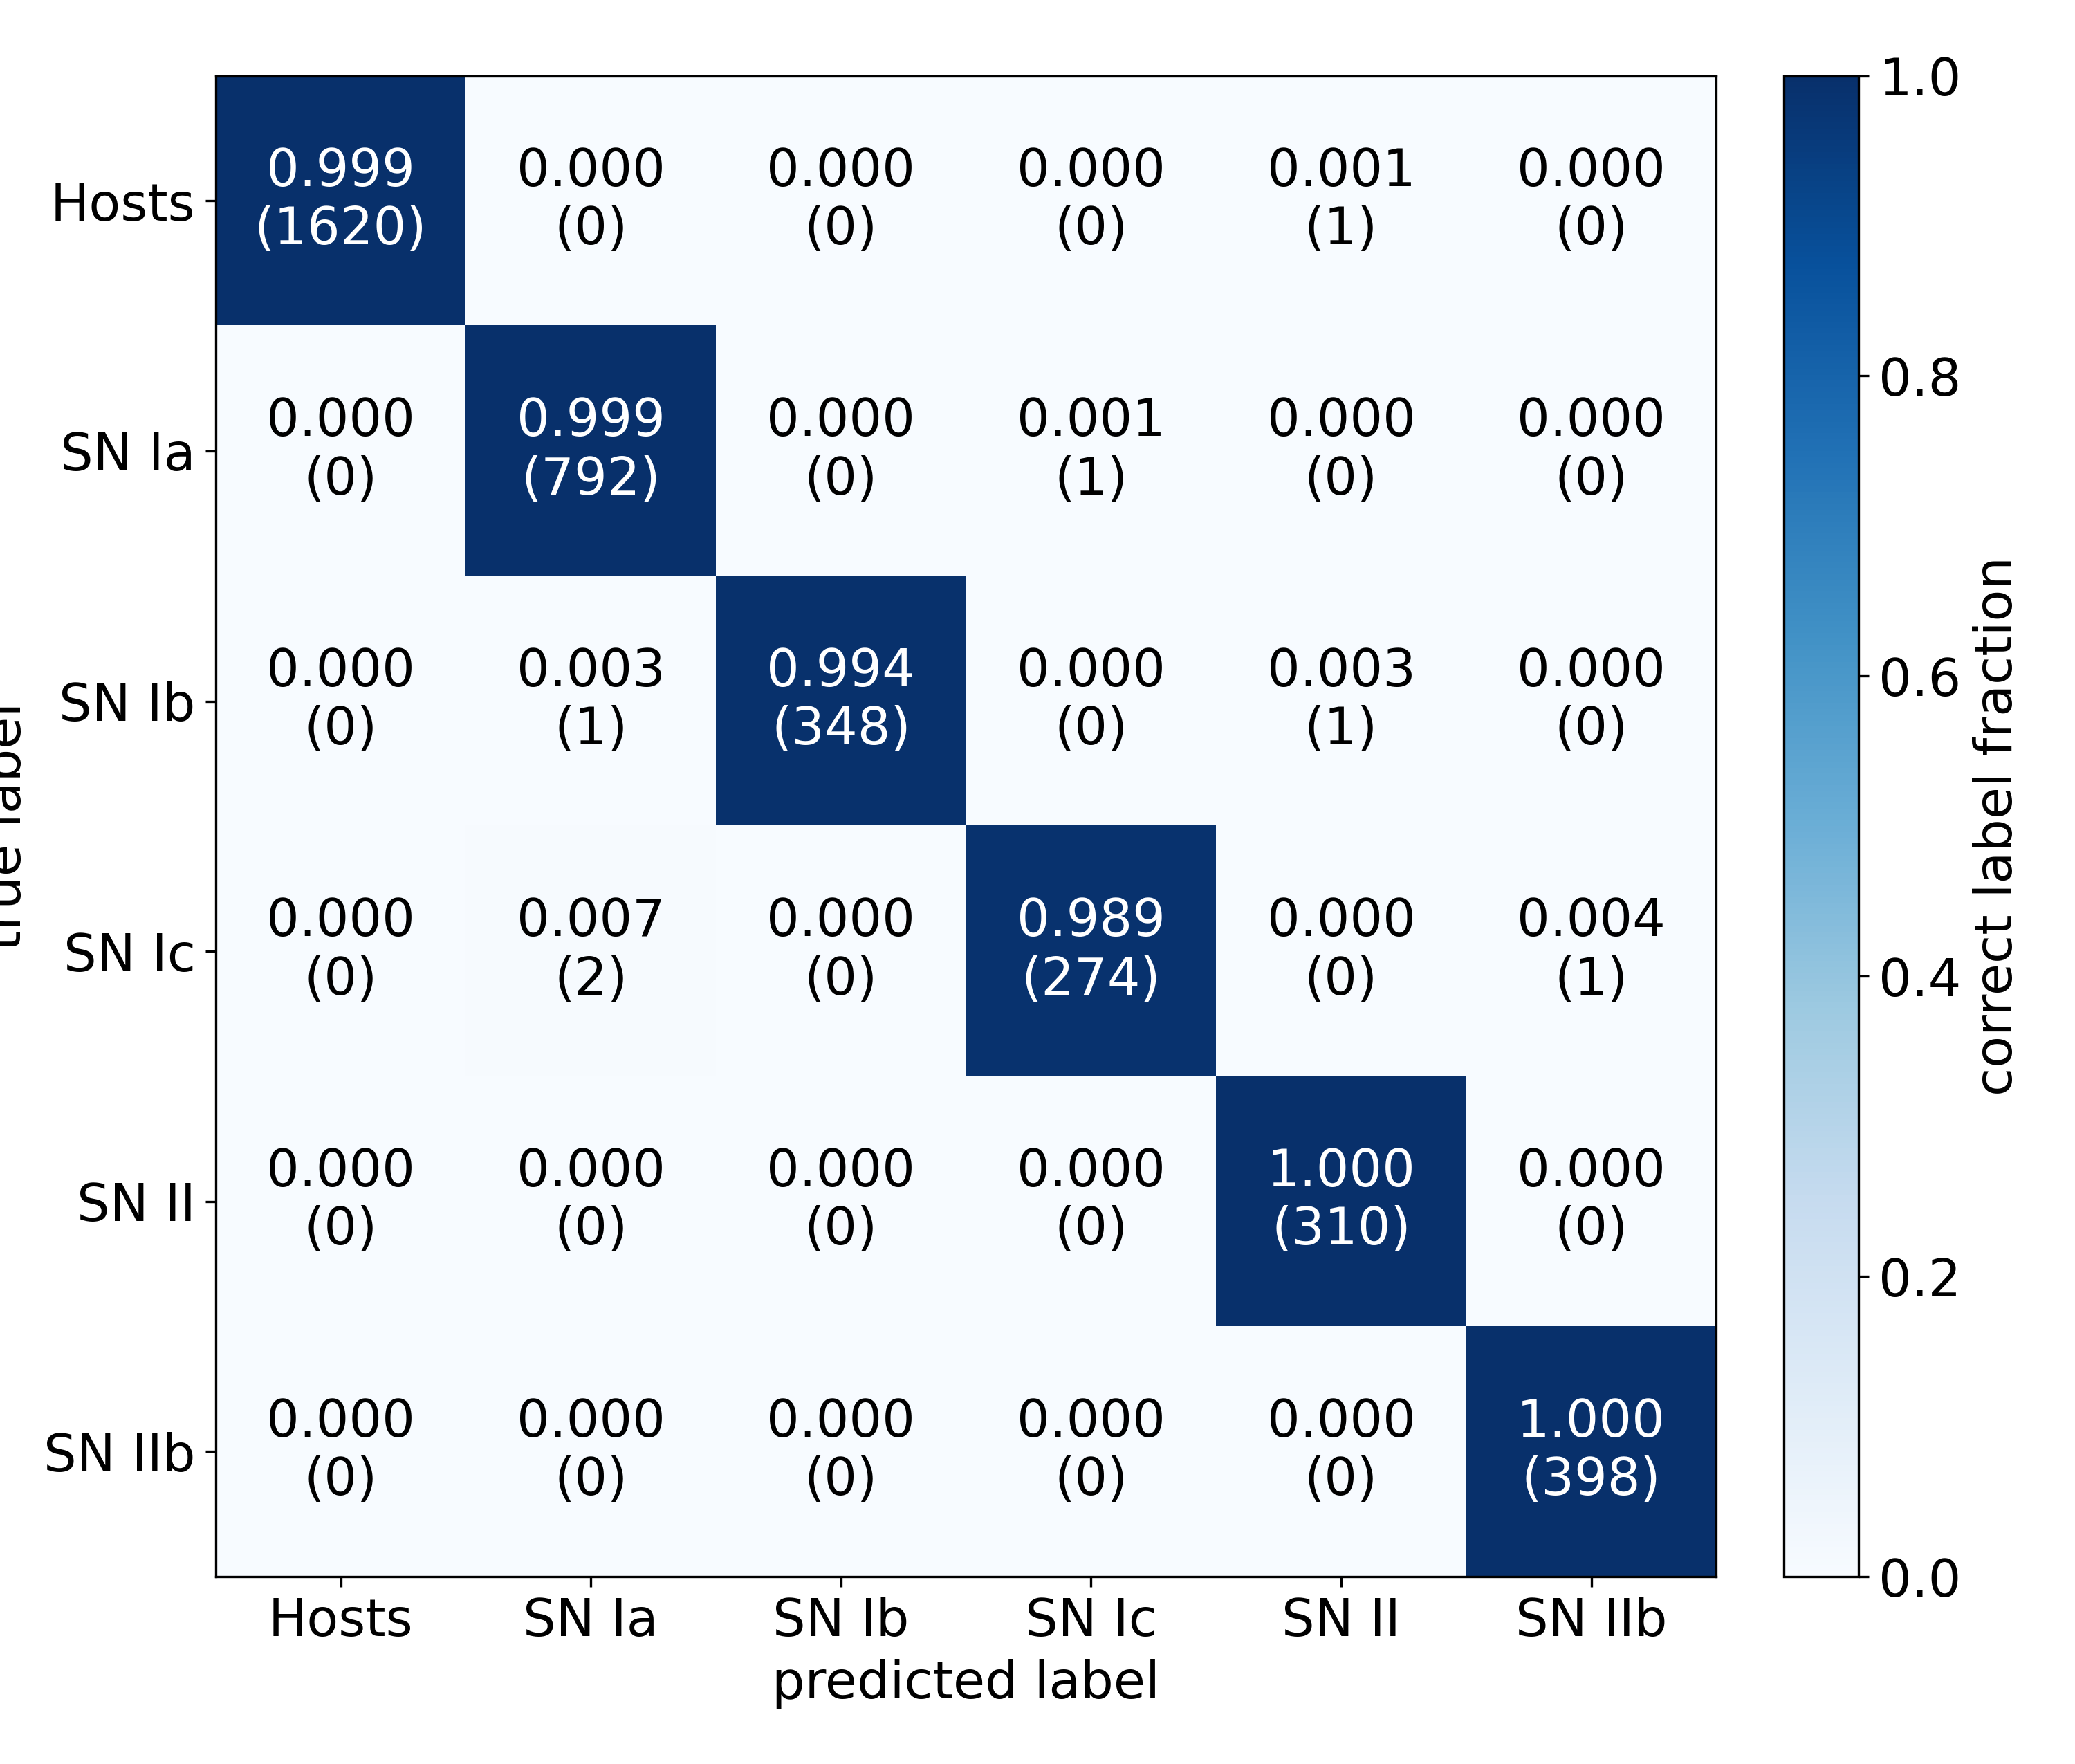
\includegraphics[height=2.6cm]{figures/cnn/cnn_cm99.png}
        \caption{CNN Classifier 99\% confidence cut (28.8\% remaining)}
    \end{figure}
\end{frame}


\begin{frame}{The Transformer Architecture}
\begin{columns}
\column{.4\textwidth}
    \begin{figure}[ht]
        \centering
        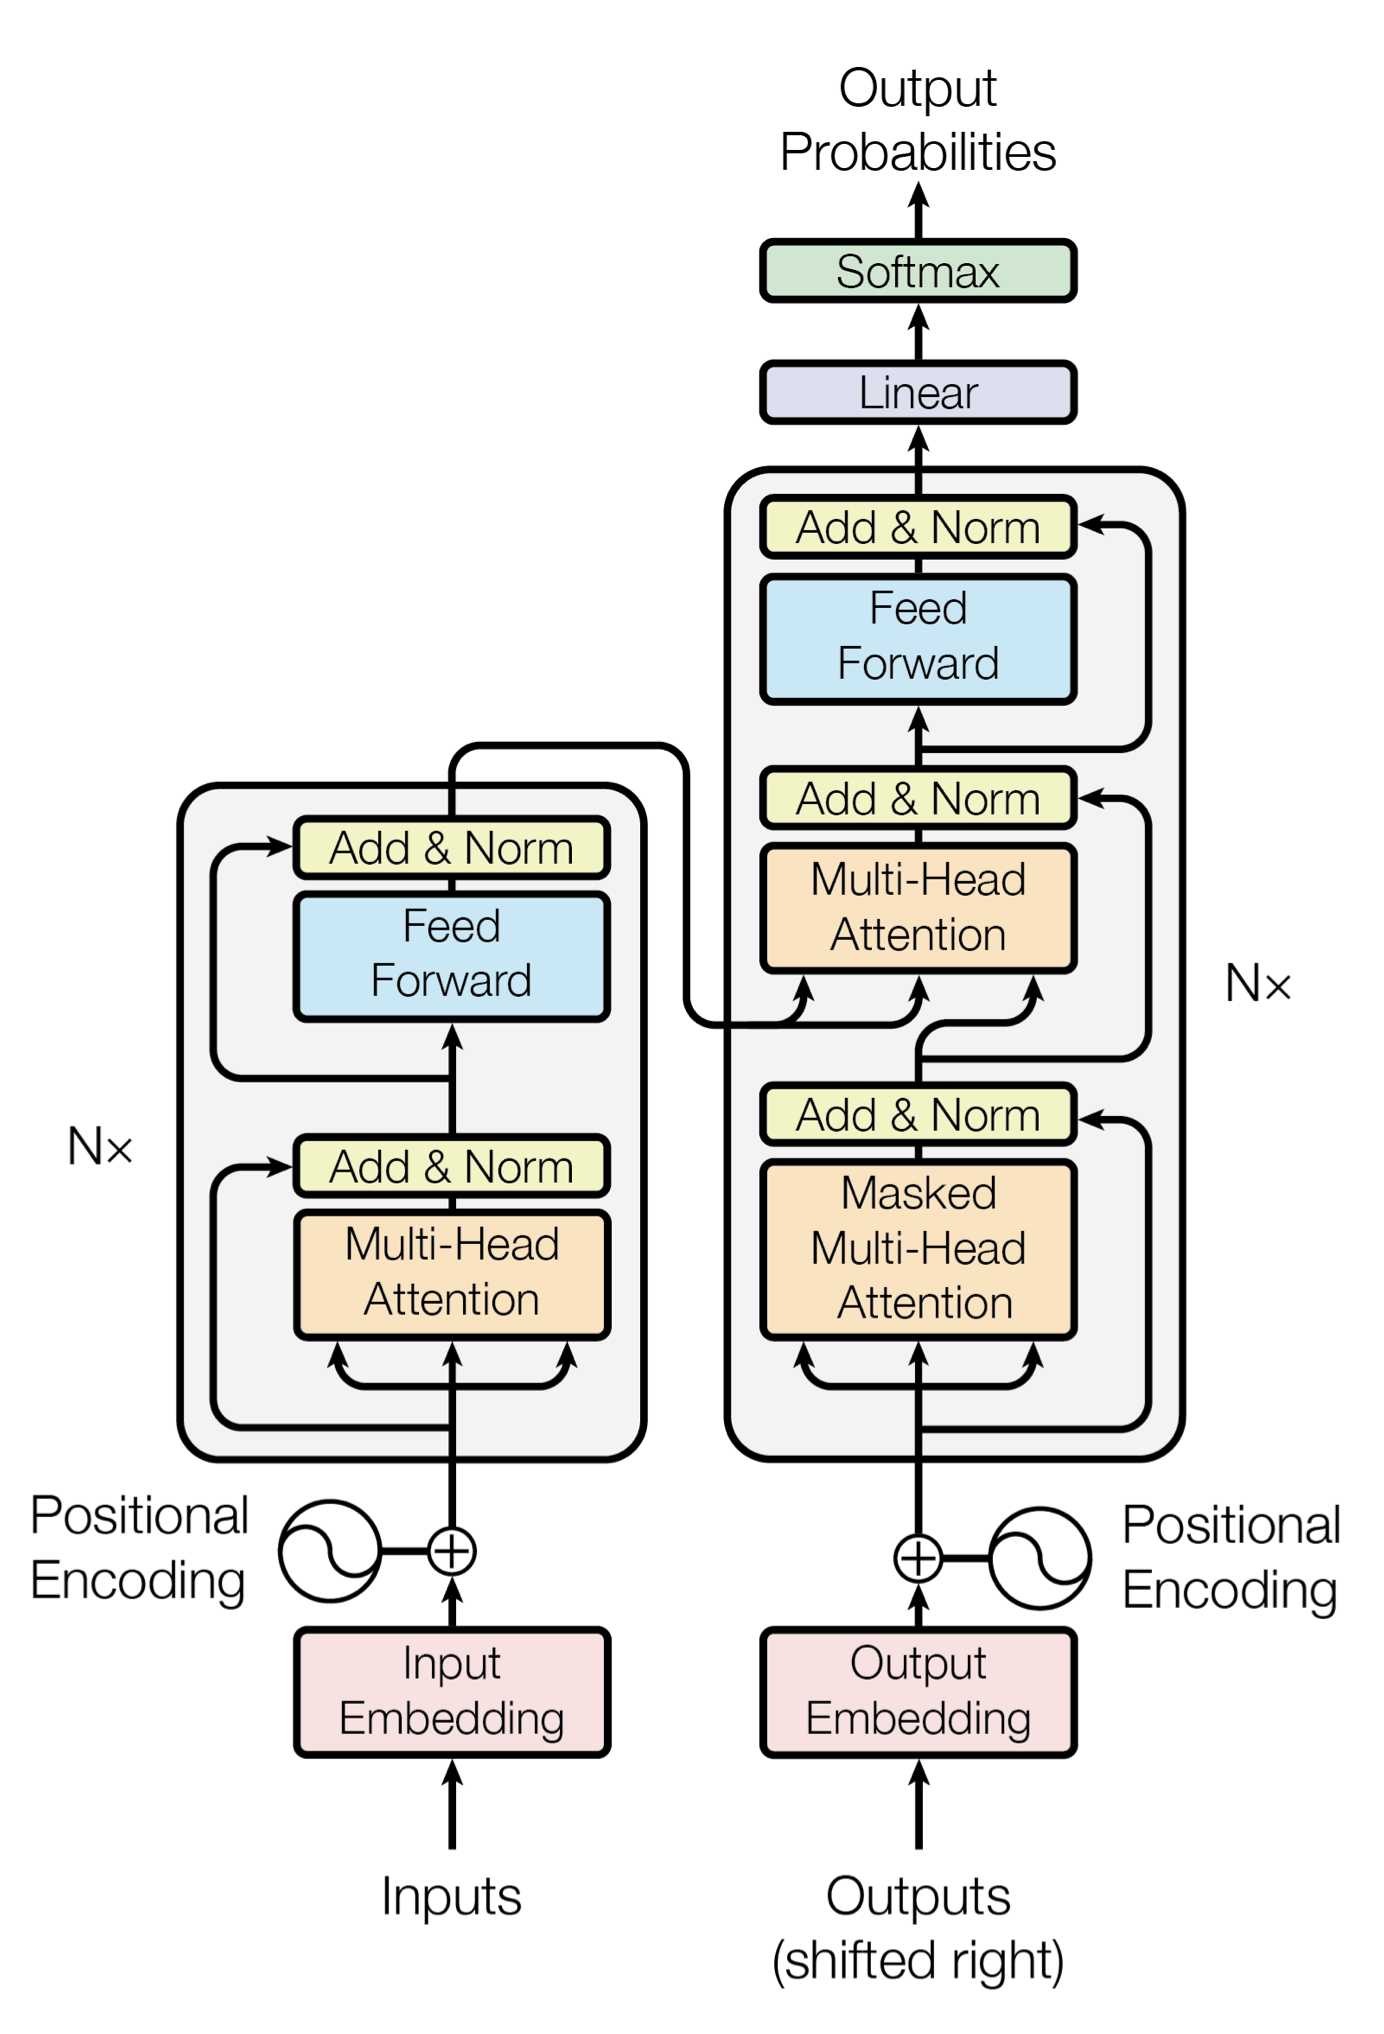
\includegraphics[width=.9\textwidth]{figures/transformer_paper/Transformer_Original.png}
        \caption{Original Transformer Architecture (Image from \textcite{vaswani2017})
        % ]{Traditional transformer architecture consisting of an enocoder and decoder. 
        \label{fig:transformer_orig}}
    \end{figure}
% \end{frame}

% \begin{frame}
\column{.58\textwidth}
    \begin{figure}[t]
        \centering
        \includegraphics[width=\textwidth]{figures/transformer_paper/ViT_Original.png}
        \caption{ViT Architecture (Image from \textcite{dosovitskiy2020})
        % ]{Vision transformer (ViT) architecture. Purple ovals indicate 
        %     positional embeddings, while pink ovals indicate the resulting tokens from 
        %     the patches. 
        \label{fig:ViT_orig}}
    \end{figure}
    \end{columns}
\end{frame}

\begin{comment}
\begin{frame}
    \begin{columns}
        \column{0.4\textwidth}
            This is an example of text and image in the same slide using columns environment.
        \column{0.6\textwidth}
            \begin{figure}
                \centering
                \includegraphics[width=\textwidth]{Neural-Network.jpg}
                \caption{Neural Network with 5 neurons in the hidden layer. }
            \end{figure}
    \end{columns}
\end{frame}

\begin{frame}
    \frametitle{HAM10000 Dataset \cite{Sagar2022}}
        {
            \small
            \begin{table}
            \centering
            \caption{HAM10000 Dataset Classes}\label{tab:HAM}
            \resizebox{.3\linewidth}{!}{\begin{tabular}{lccc}
	\toprule
    \textbf{Spam} & \textbf{Ni} & \textbf{Swallow} & \textbf{Shrubbery} \\
    \midrule
    A & 1 & 2 & 3 \\
    \midrule
    E & 3 & 4 & 5 \\
    C & 6 & 9 & 3 \\
    \midrule
    M & 4 & 1 & 1 \\
    \bottomrule
\end{tabular}}
            \end{table}
        }
        \begin{figure}
            \centering
            
\includegraphics[width=0.3\textwidth]{figures/blackbox.jpeg}
            \caption{Example of HAM10000 dataset with true classes and segmentation}
        \end{figure}
\end{frame}
%%%%%%%%%%%%%%%%%%%%%%%%%%%%%%%%%%%%%%%%%%%%%%%%%%%%%%%%%%%%%%%%%%%%%%%%
\begin{frame}
    \frametitle{Classification Models}
    \small
    \begin{table}[]
        \centering
        \caption{Models}\label{tab:models}
        \resizebox{\linewidth}{!}{\begin{tabular}{lccc}
	\toprule
    \textbf{Spam} & \textbf{Ni} & \textbf{Swallow} & \textbf{Shrubbery} \\
    \midrule
    A & 1 & 2 & 3 \\
    \midrule
    E & 3 & 4 & 5 \\
    C & 6 & 9 & 3 \\
    \midrule
    M & 4 & 1 & 1 \\
    \bottomrule
\end{tabular}}
    \end{table}
    
\end{frame}
\end{comment}

%%%%%%%%%%%%%%%%%%%%%%%%%%%%%%%%%%%%%%%%%%%%%%%%%%%%%%%%%%%%%%%%%%%%%%%%

\section[Spectral ViT]{Creation and Training of the Spectral ViT}
%%%%%%%%%%%%%%%%%%%%%%%%%%%%%%%%%%%%%%%%%%%%%%%%%%%%%%%%%%%%%%%%%%%%%%%%
%%%%%%%%%%%%%%%%%%%%%%%%%%%%%%%%%%%%%%%%%%%%%%%%%%%%%%%%%%%%%%%%%%%%%%%%
\begin{frame}{Spectral ViT}
\begin{columns}[c]
\column{.4\textwidth}
Transformer architecture must satisfy 
    \begin{itemize}
        \item 1D Nature of Spectra (more like original transformer)
        \item Cut up data into `patches' synthetically (more like ViT)
    \end{itemize}
\column{.5\textwidth}
    \begin{figure}
        \centering
        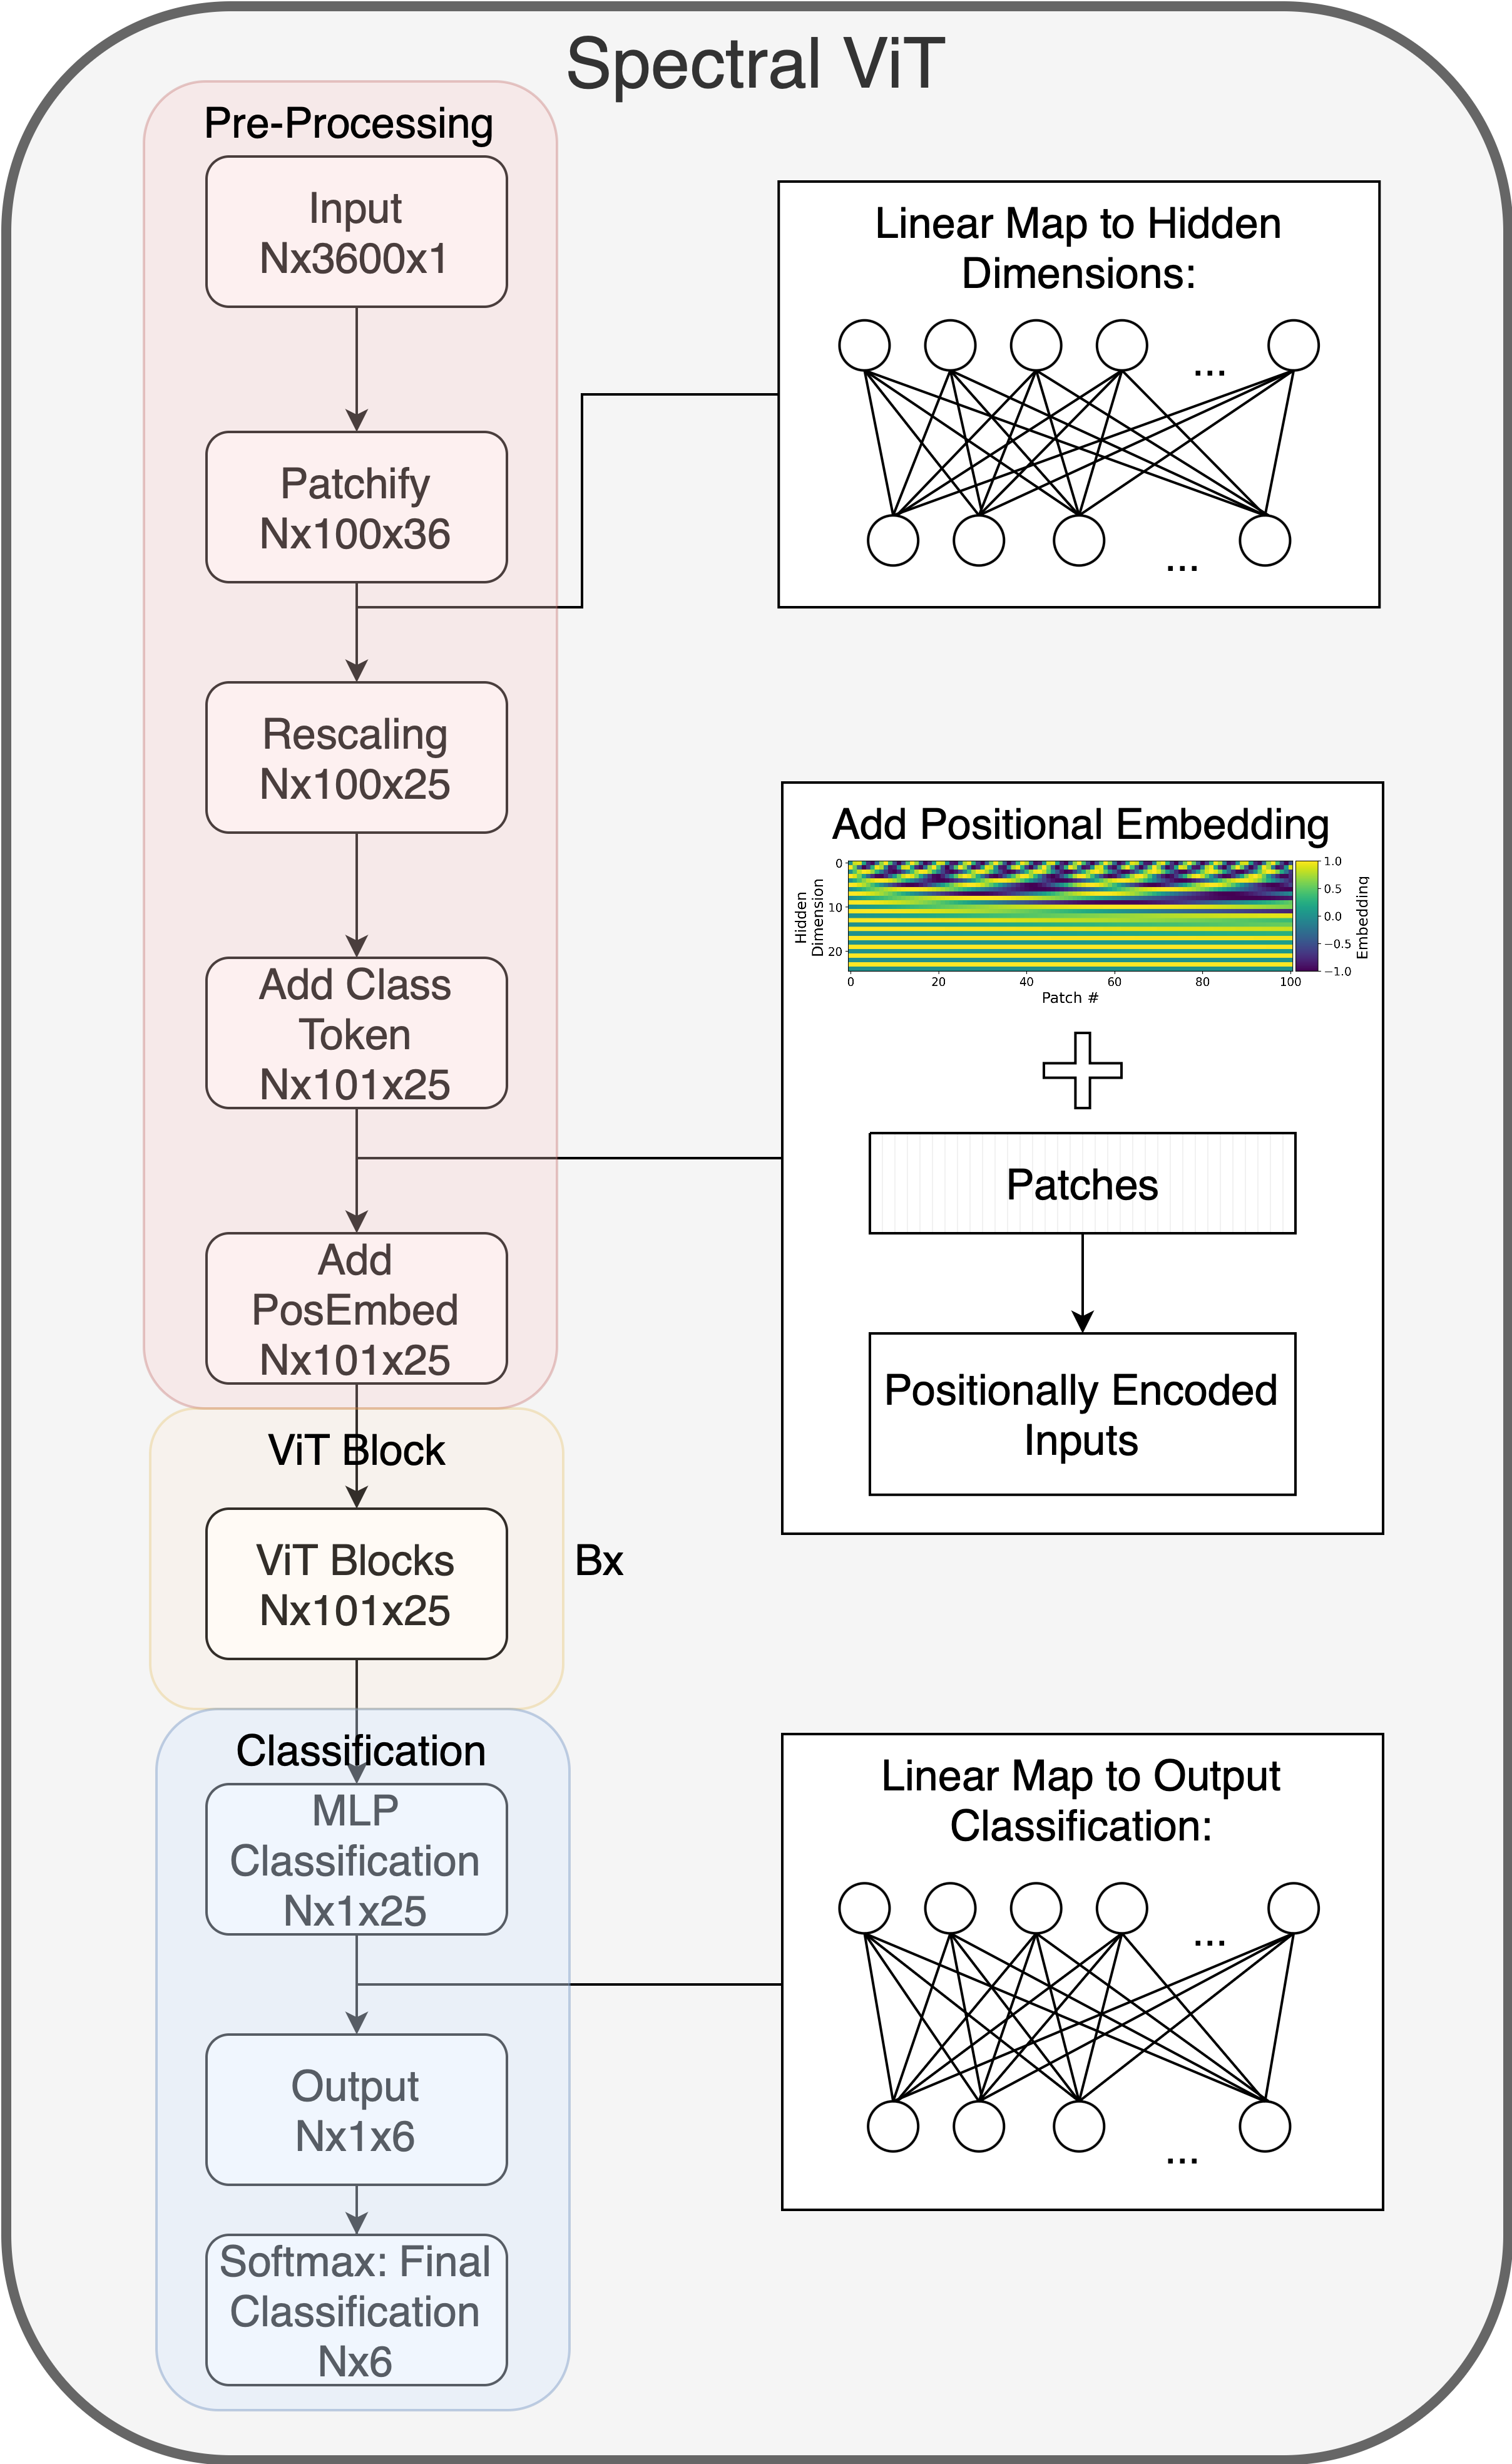
\includegraphics[width=.8\textwidth]{figures/TransformerDiagrams/SpectralViT_Presentation.png}
    \end{figure}
\end{columns}
\end{frame}

%%%%%%%%%%%%%%%%%%%%%%%%%%%%%%%%%%%%%%%%%%%%%%%%%%%%%%%%%%%%%%%%%%%%%%%%
\begin{frame}{Positional Embedding}
    \begin{equation}
        \text{Embedding}_{ij} = \begin{cases} \sin\left(\frac{i}{10000^{(j / \text{patch size})}}\right) & \text{if } j \text{ is even} \\
        \cos\left(\frac{i}{10000^{((j - 1) / \text{patch size})}}\right) & \text{if } j \text{ is odd}\end{cases}
    \end{equation}
    \pause
    \begin{figure}[t]
        \centering
        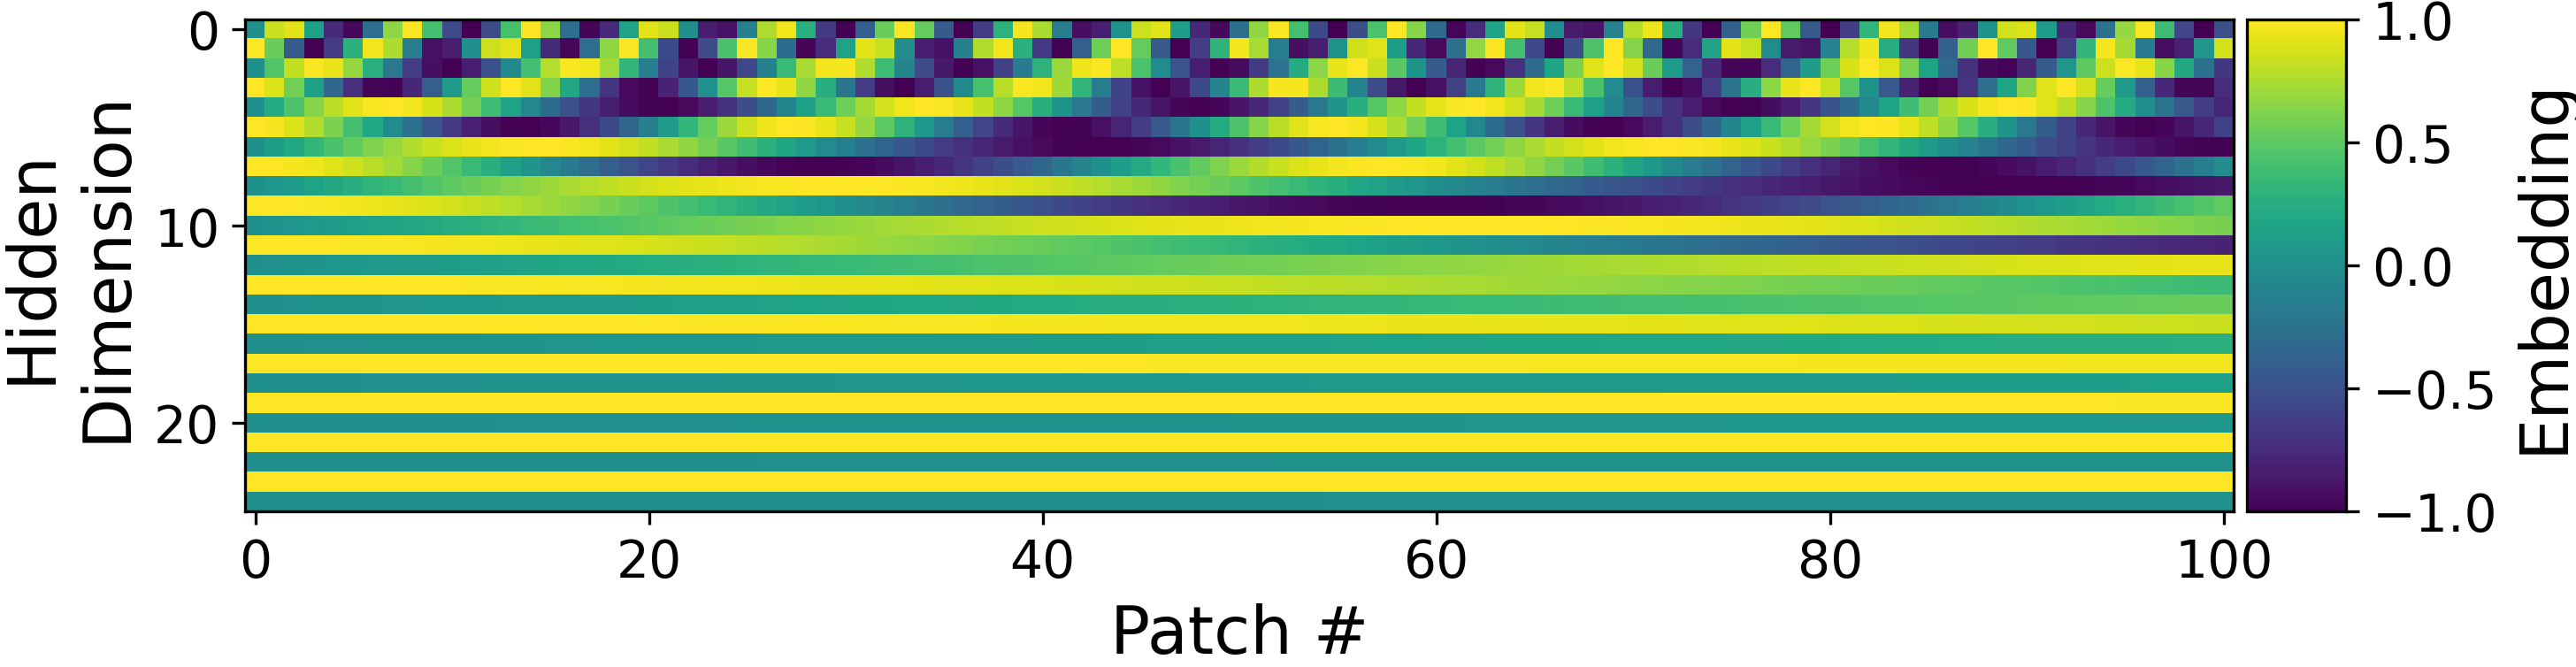
\includegraphics[width=.9\linewidth]{figures/embeddings_new.png}
        \caption{Positional Embeddings for ViT}
    %     {Visual representation of the embeddings for a sample of spectra. The x-axis represents the 
    %     index of the patch, the y-axis represents the index of the hidden dimension, and the color represents 
    % the value of the embedding.}
        \label{fig:embedding}
    \end{figure}
\end{frame}

%%%%%%%%%%%%%%%%%%%%%%%%%%%%%%%%%%%%%%%%%%%%%%%%%%%%%%%%%%%%%%%%%%%%%%%%
\begin{frame}{Attention}
    \begin{equation}
        \label{eq:mhsa}
        \text{Attention}(Q, K, V) = \text{softmax}\left(\frac{Q\cdot K^T}{\sqrt{d_k}}\right)\cdot V
    \end{equation}
    \pause
    \begin{figure}
        \centering 
        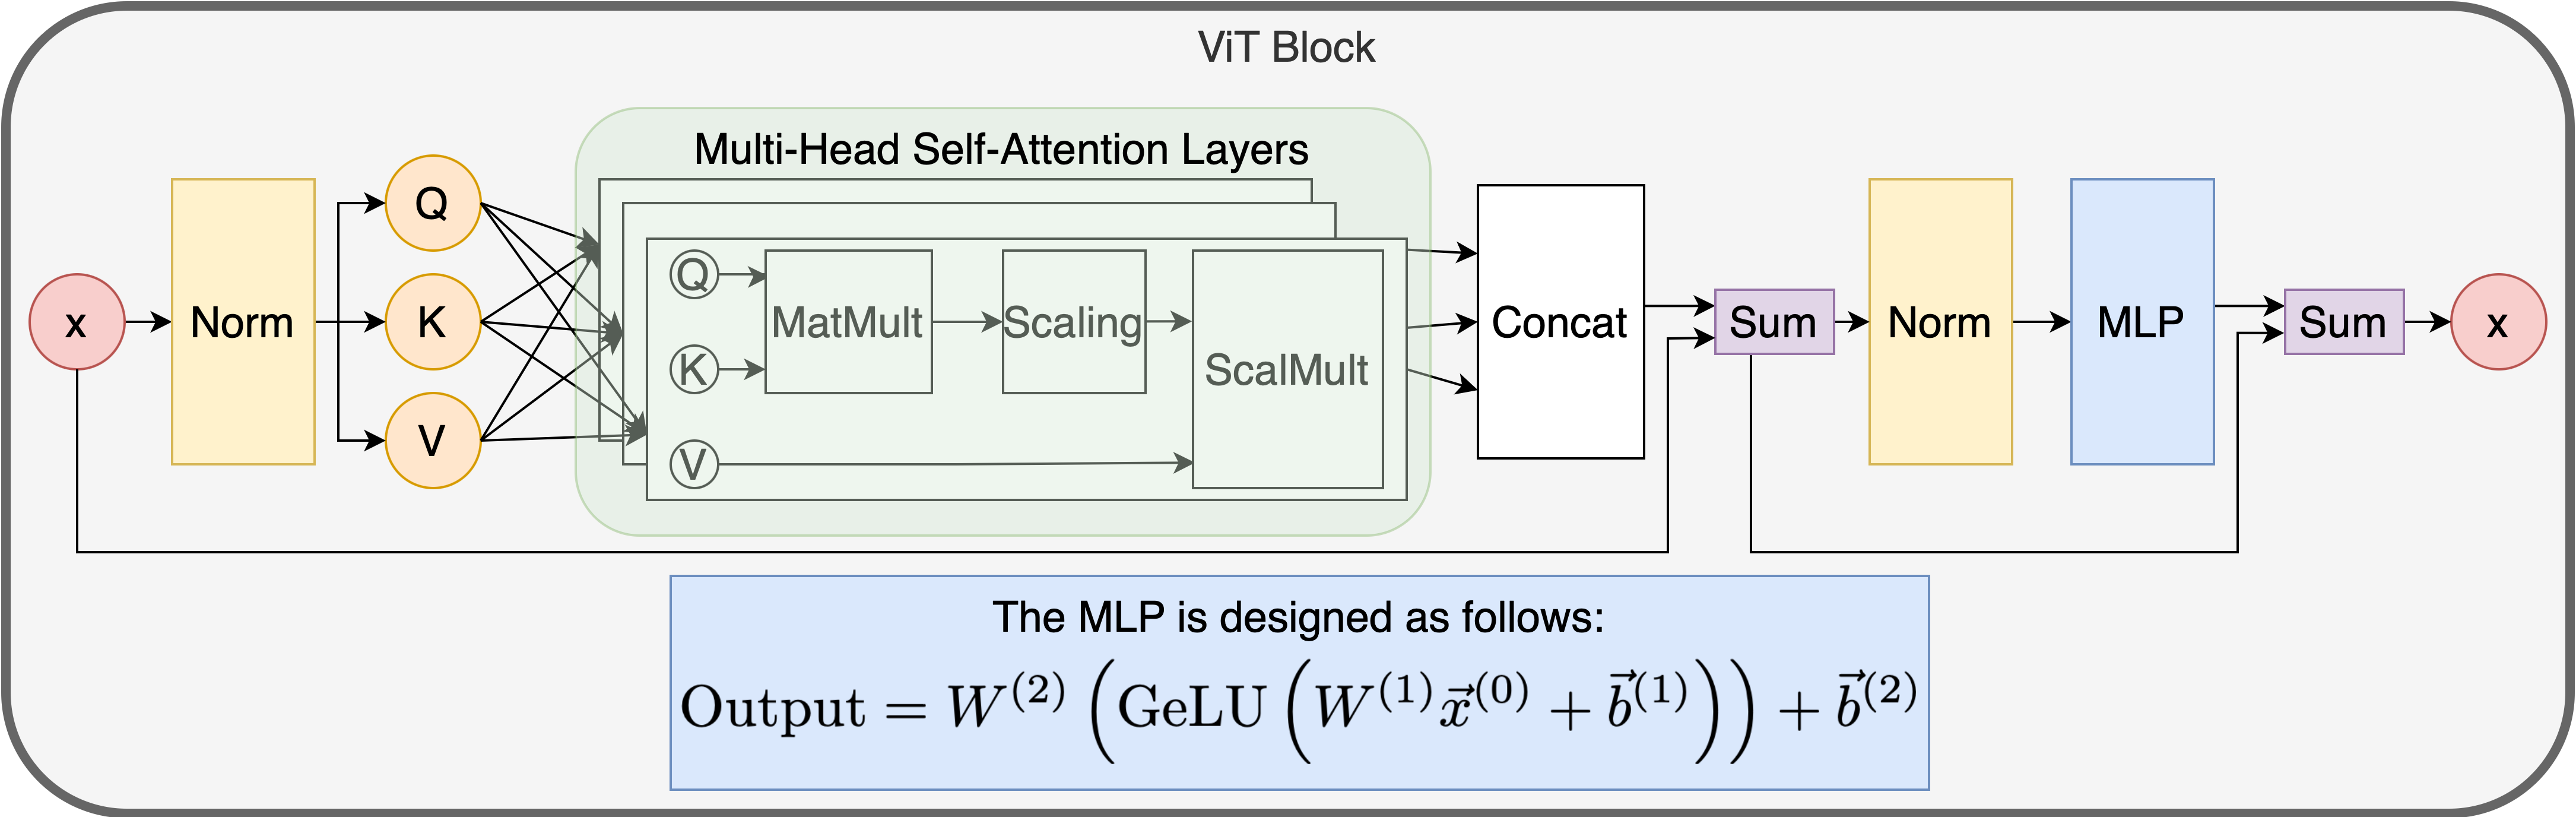
\includegraphics[width=.9\textwidth]{figures/TransformerDiagrams/Attention_Presentation.png}
        \caption{ViT Block Architecture for the Spectral ViT}
        \label{fig:SpectralViTBlock}
    \end{figure}
\end{frame}

%%%%%%%%%%%%%%%%%%%%%%%%%%%%%%%%%%%%%%%%%%%%%%%%%%%%%%%%%%%%%%%%%%%%%%%%
\begin{frame}{Final Architecture}
\begin{columns}[c]
\column{.38\textwidth}
    \begin{figure}
        \centering
        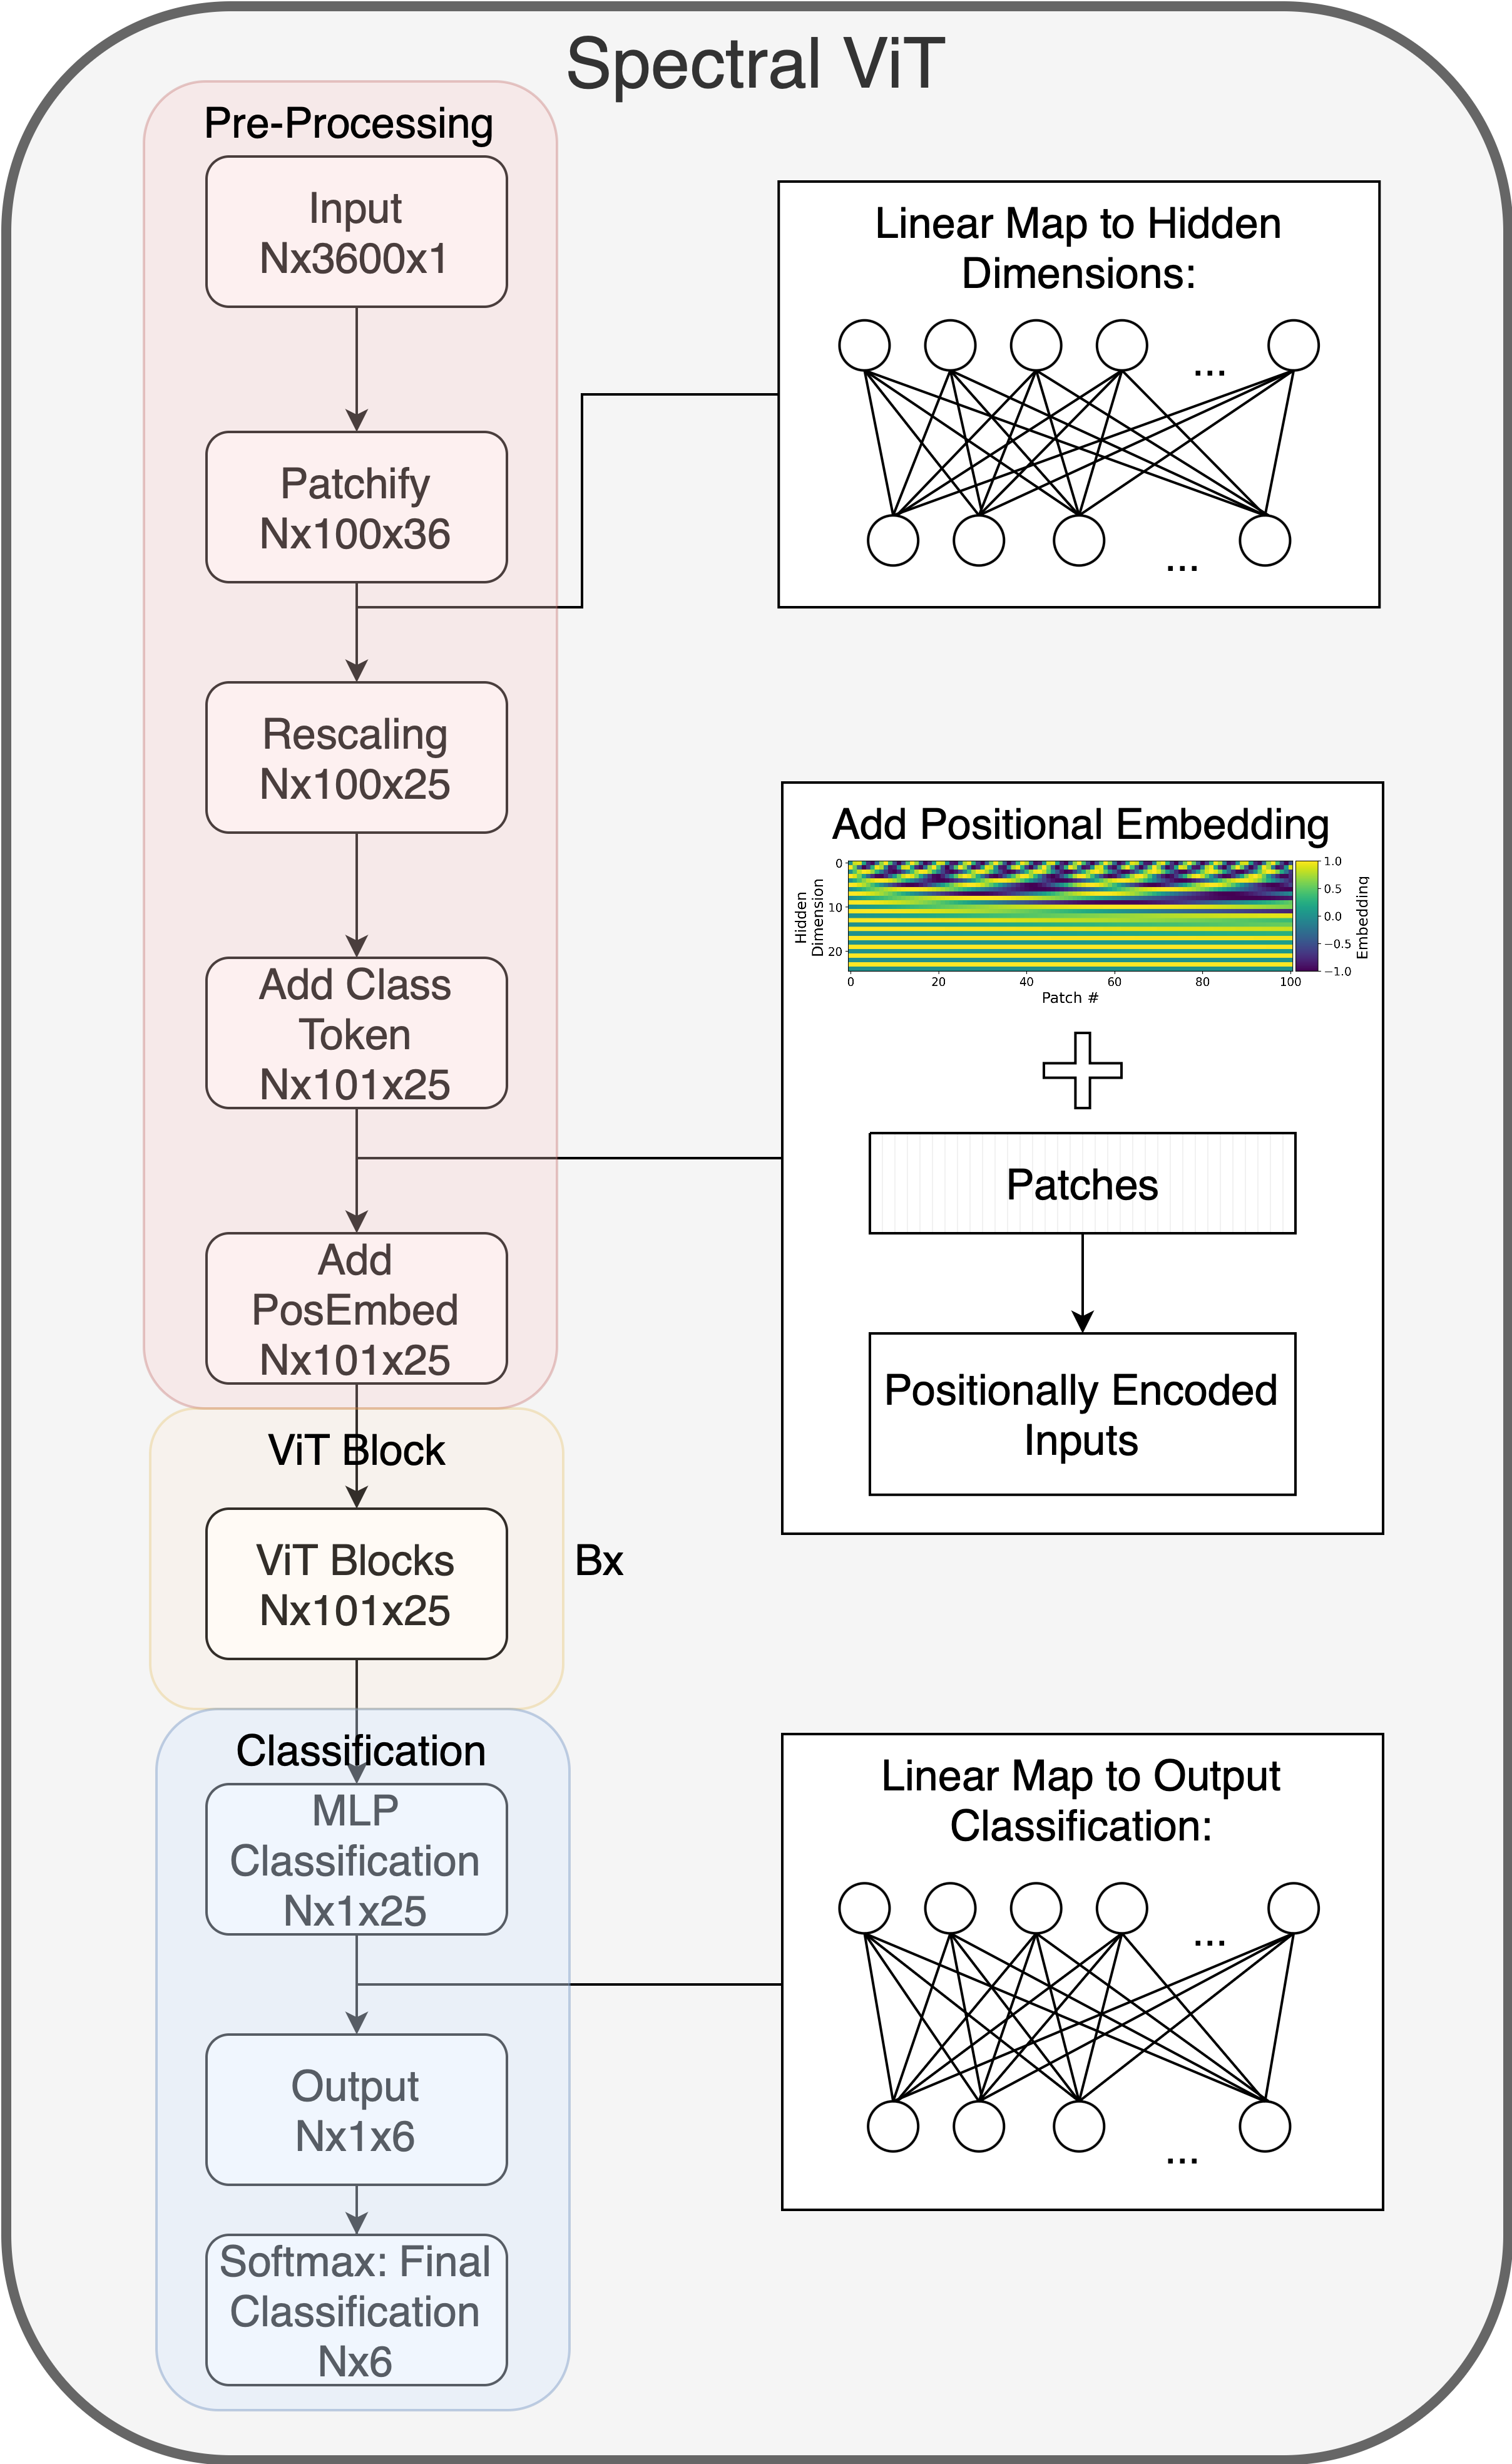
\includegraphics[width=\textwidth]{figures/TransformerDiagrams/SpectralViT_Presentation.png}
    \end{figure}
\column{.58\textwidth}
    \begin{figure}
        \centering
        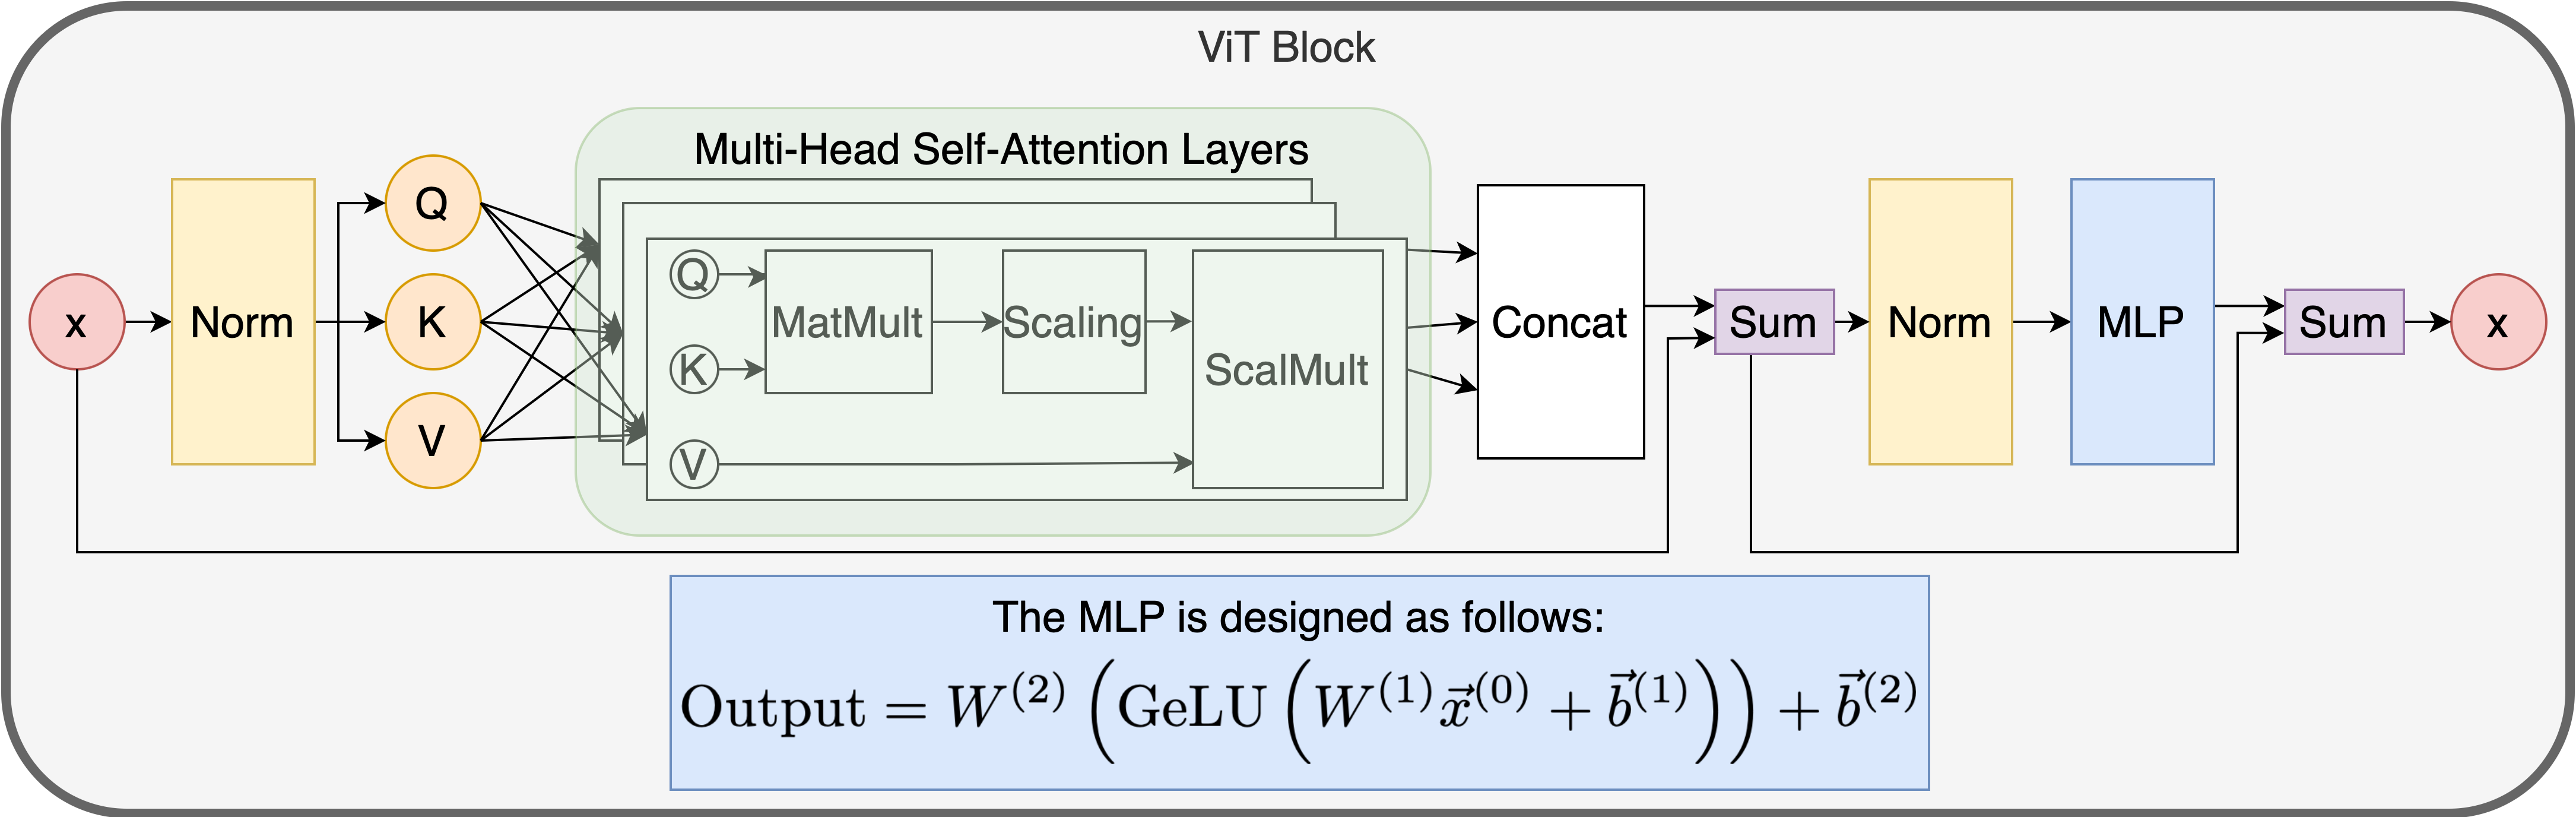
\includegraphics[width=\textwidth]{figures/TransformerDiagrams/Attention_Presentation.png}
    \end{figure}
\end{columns}
\end{frame}
%%%%%%%%%%%%%%%%%%%%%%%%%%%%%%%%%%%%%%%%%%%%%%%%%%%%%%%%%%%%%%%%%%%%%%%%
\begin{frame}
    \begin{figure}[t]
        \centering
        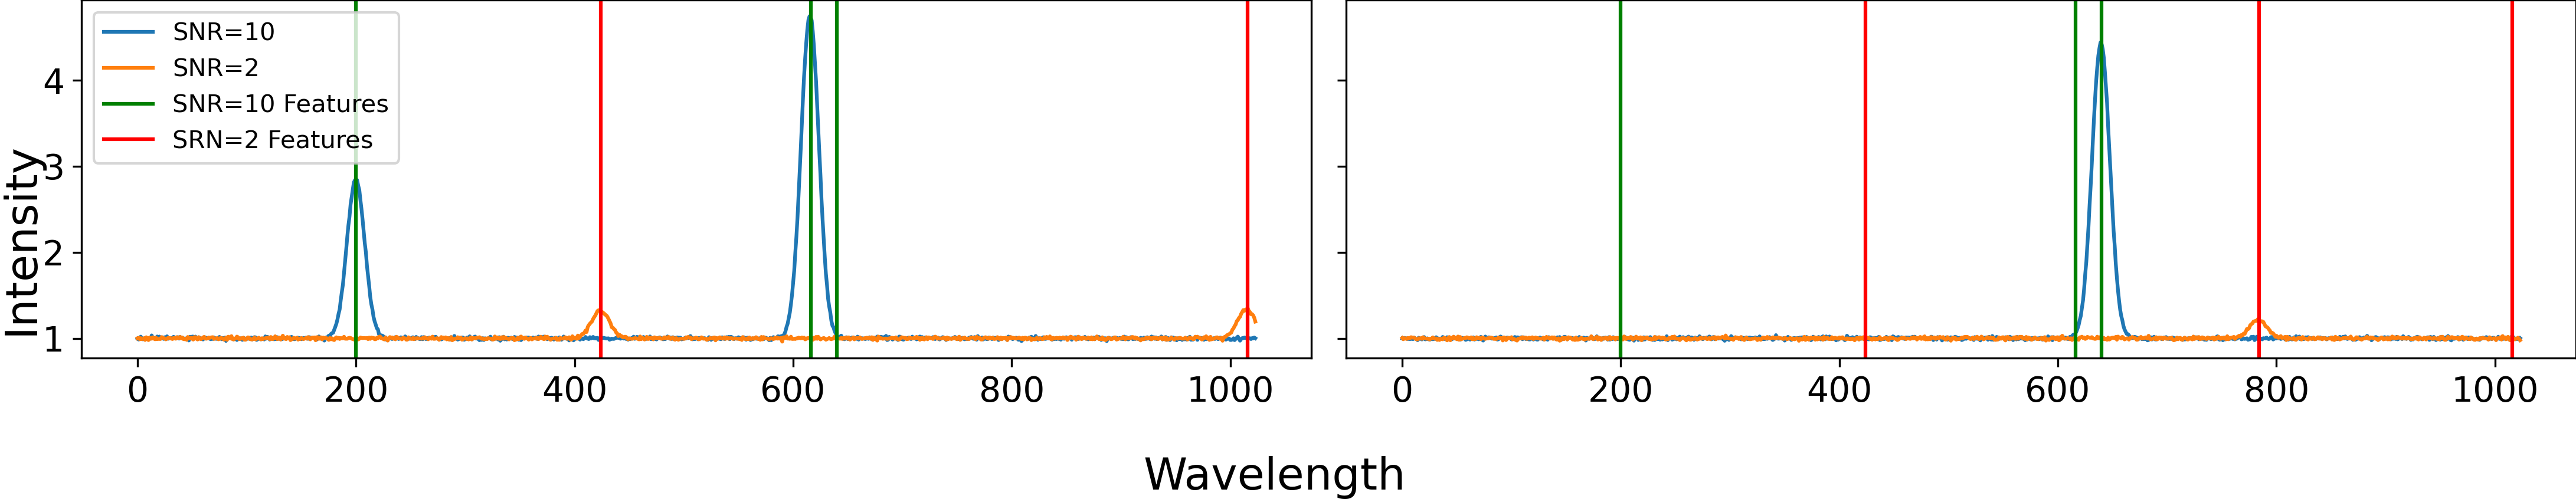
\includegraphics[width=\textwidth]{figures/synth_data_new.png}
        \caption[Synthetic spectra]{Synthetic spectra used to verify the performance of Spectral~ViT. Red and green vertical lines represent features used to 
        separate the data into distinct classes for SNR=2 and SNR=10, respectively. Two classes are shown for each SNR.}
        \label{fig:synth_spectra}
    \end{figure}
\end{frame}


%%%%%%%%%%%%%%%%%%%%%%%%%%%%%%%%%%%%%%%%%%%%%%%%%%%%%%%%%%%%%%%%%%%%%%%%
\begin{frame}
    \begin{figure}[t]
        \centering
        \subfloat[\centering~SNR = 2\label{fig:snr2}]{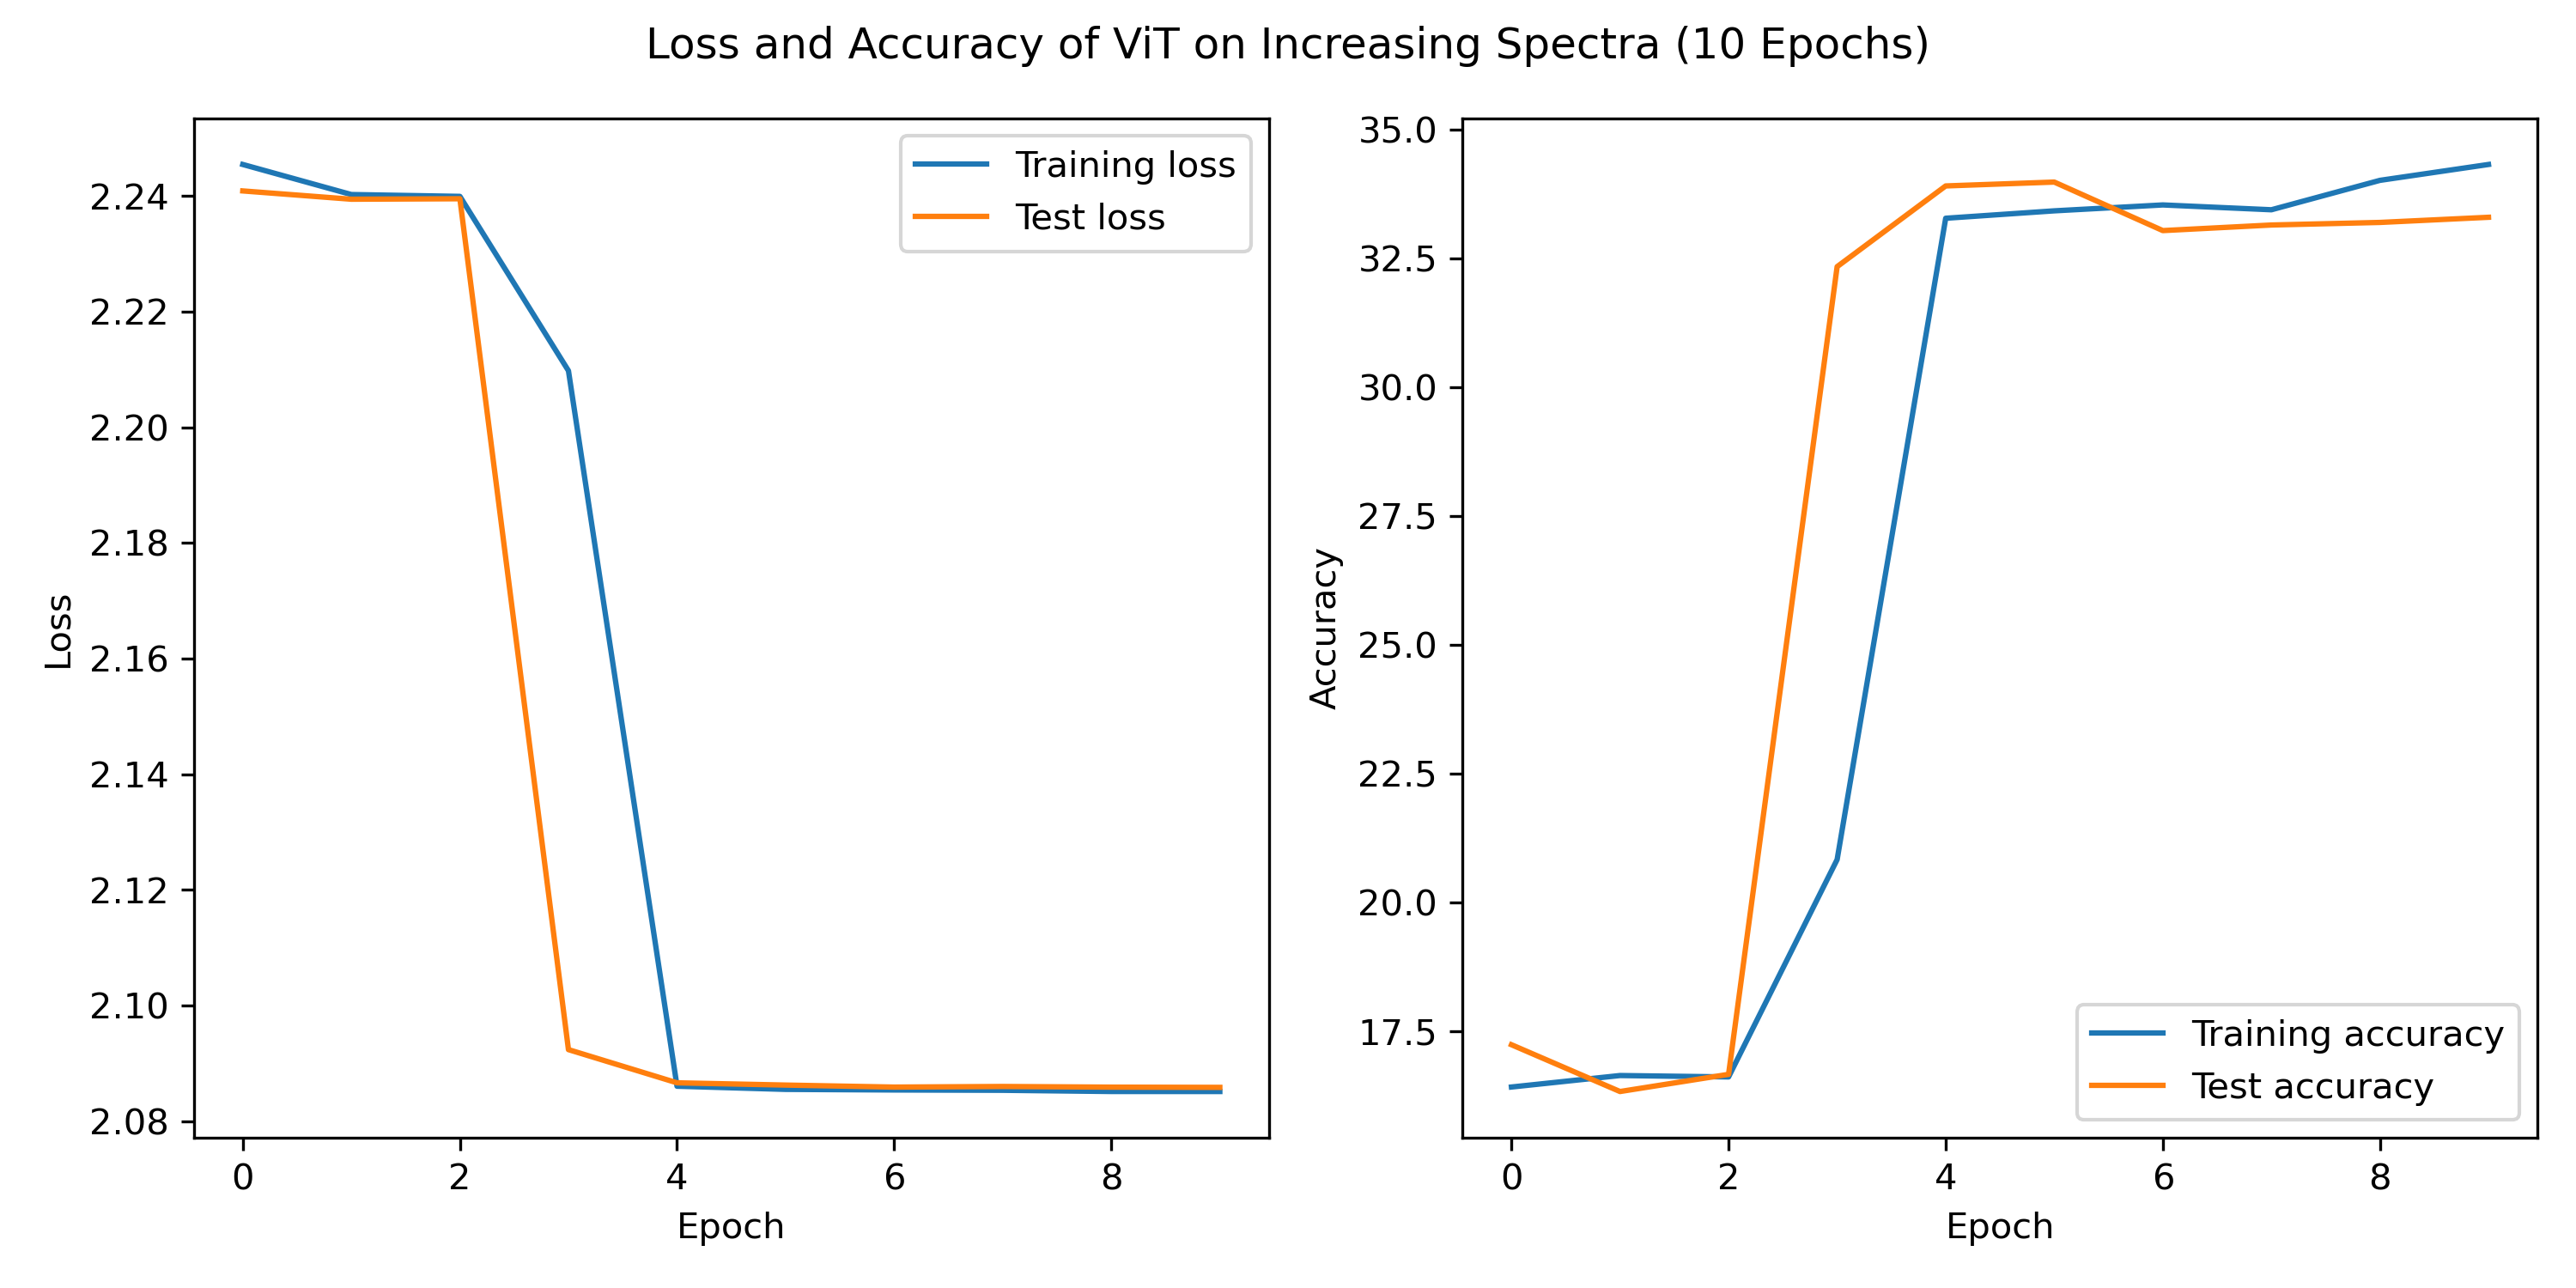
\includegraphics[width=11cm]{figures/pre_testing/SNR2_training_epoch.png}}
        \qquad
        \subfloat[\centering~SNR = 10\label{fig:snr10}]{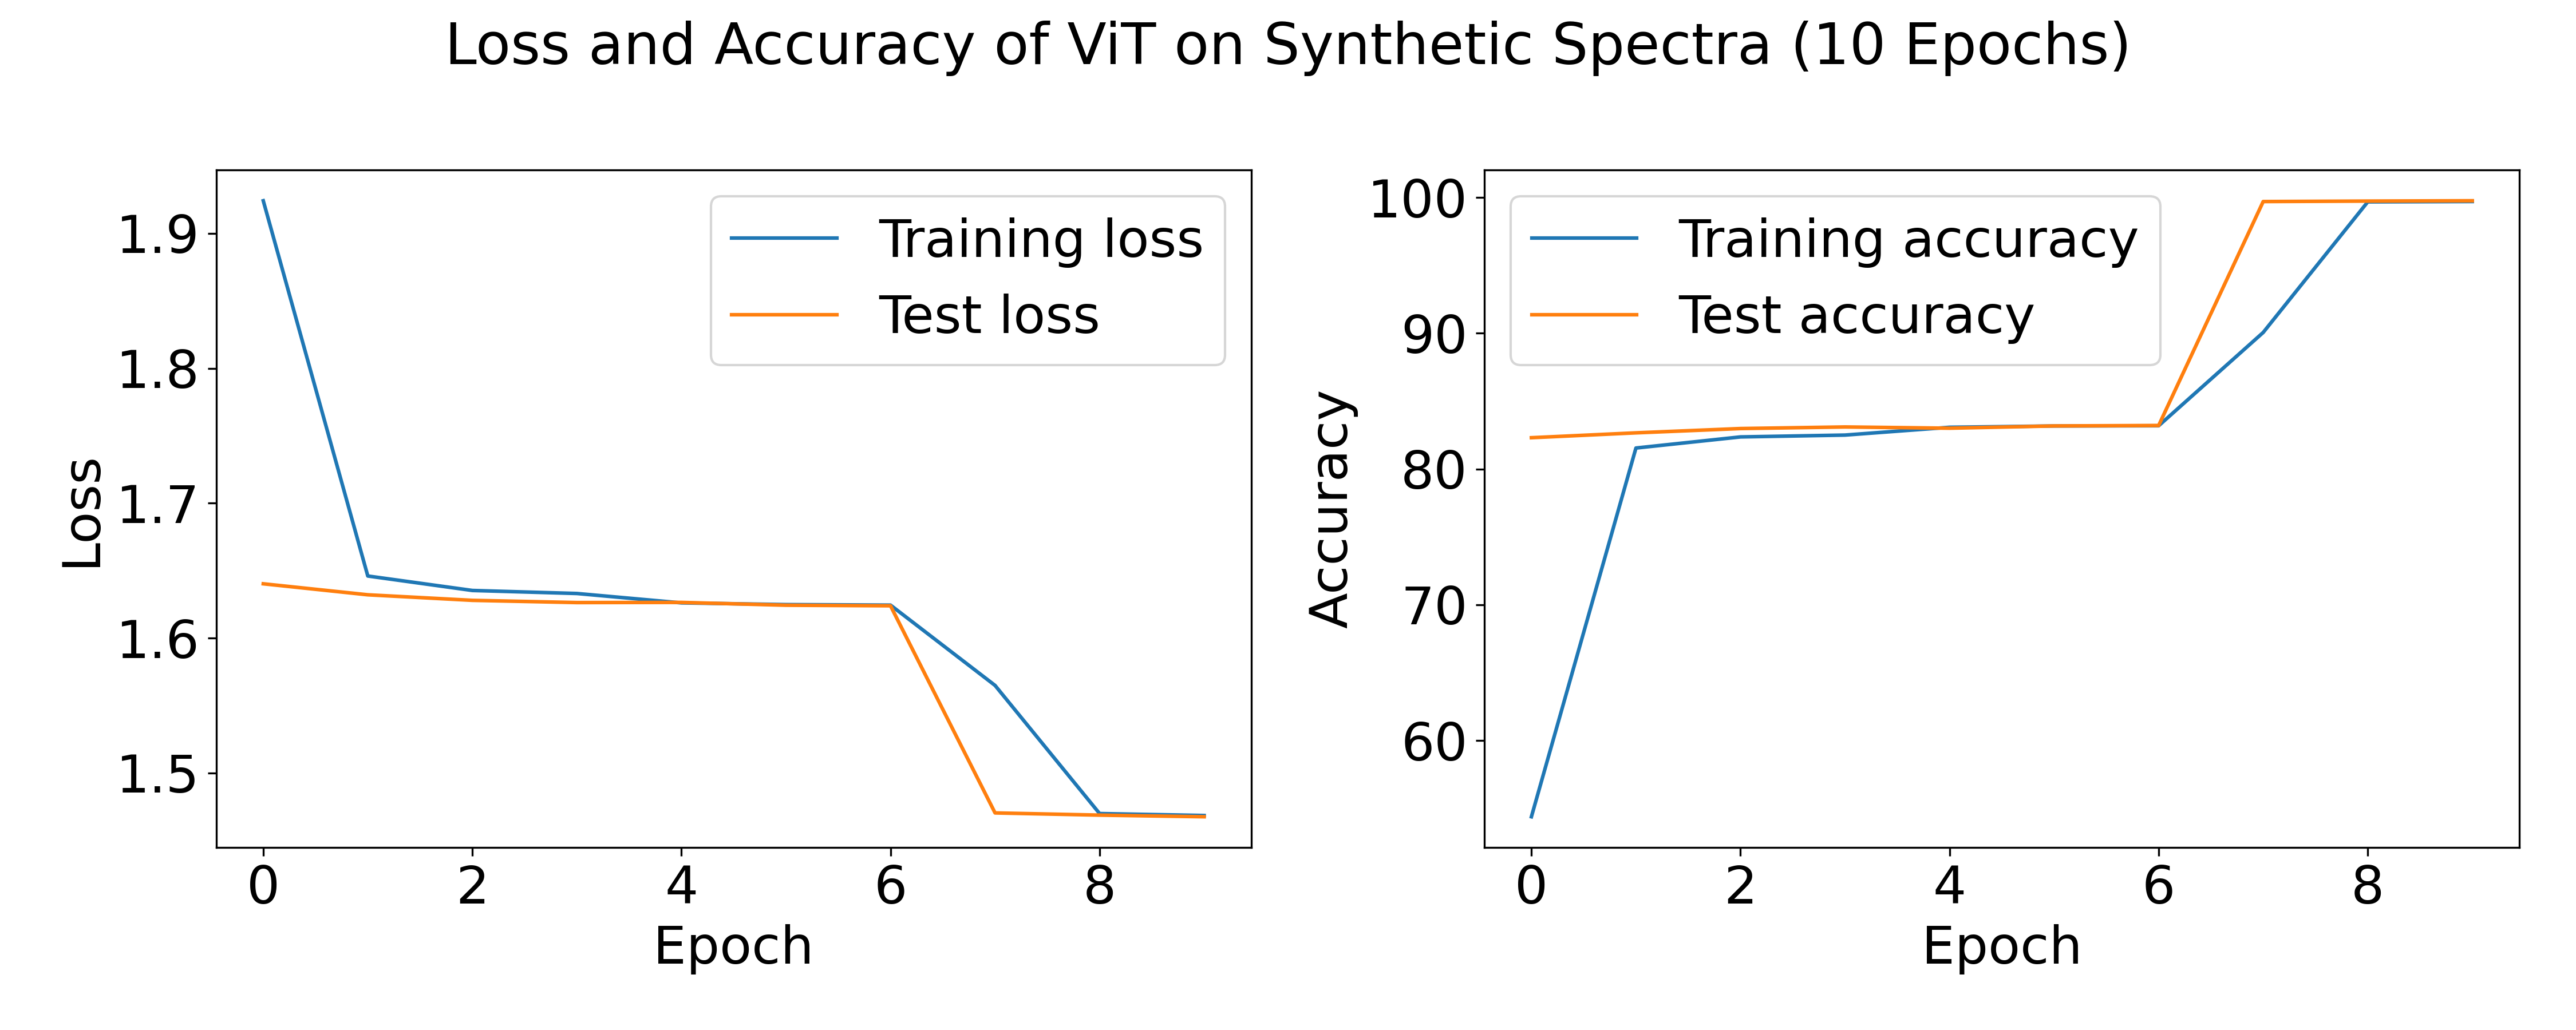
\includegraphics[width=11cm]{figures/pre_testing/SNR10_training_epoch.png}}
        \caption[Verification of ViT: Synthetic Dataset]{Training of Spectral ViT on synthetic datasets. The model was able to reach 100\% accuracy on the test set of SNR=10 (top), 
        but failed to reach an accuracy of 50\% on the test set of SNR=2 (bottom).}
    \label{fig:synth_spectra_training}
    \end{figure}
\end{frame}

%%%%%%%%%%%%%%%%%%%%%%%%%%%%%%%%%%%%%%%%%%%%%%%%%%%%%%%%%%%%%%%%%%%%%%%%
\begin{frame}
    \begin{figure}[t!]
        \centering
        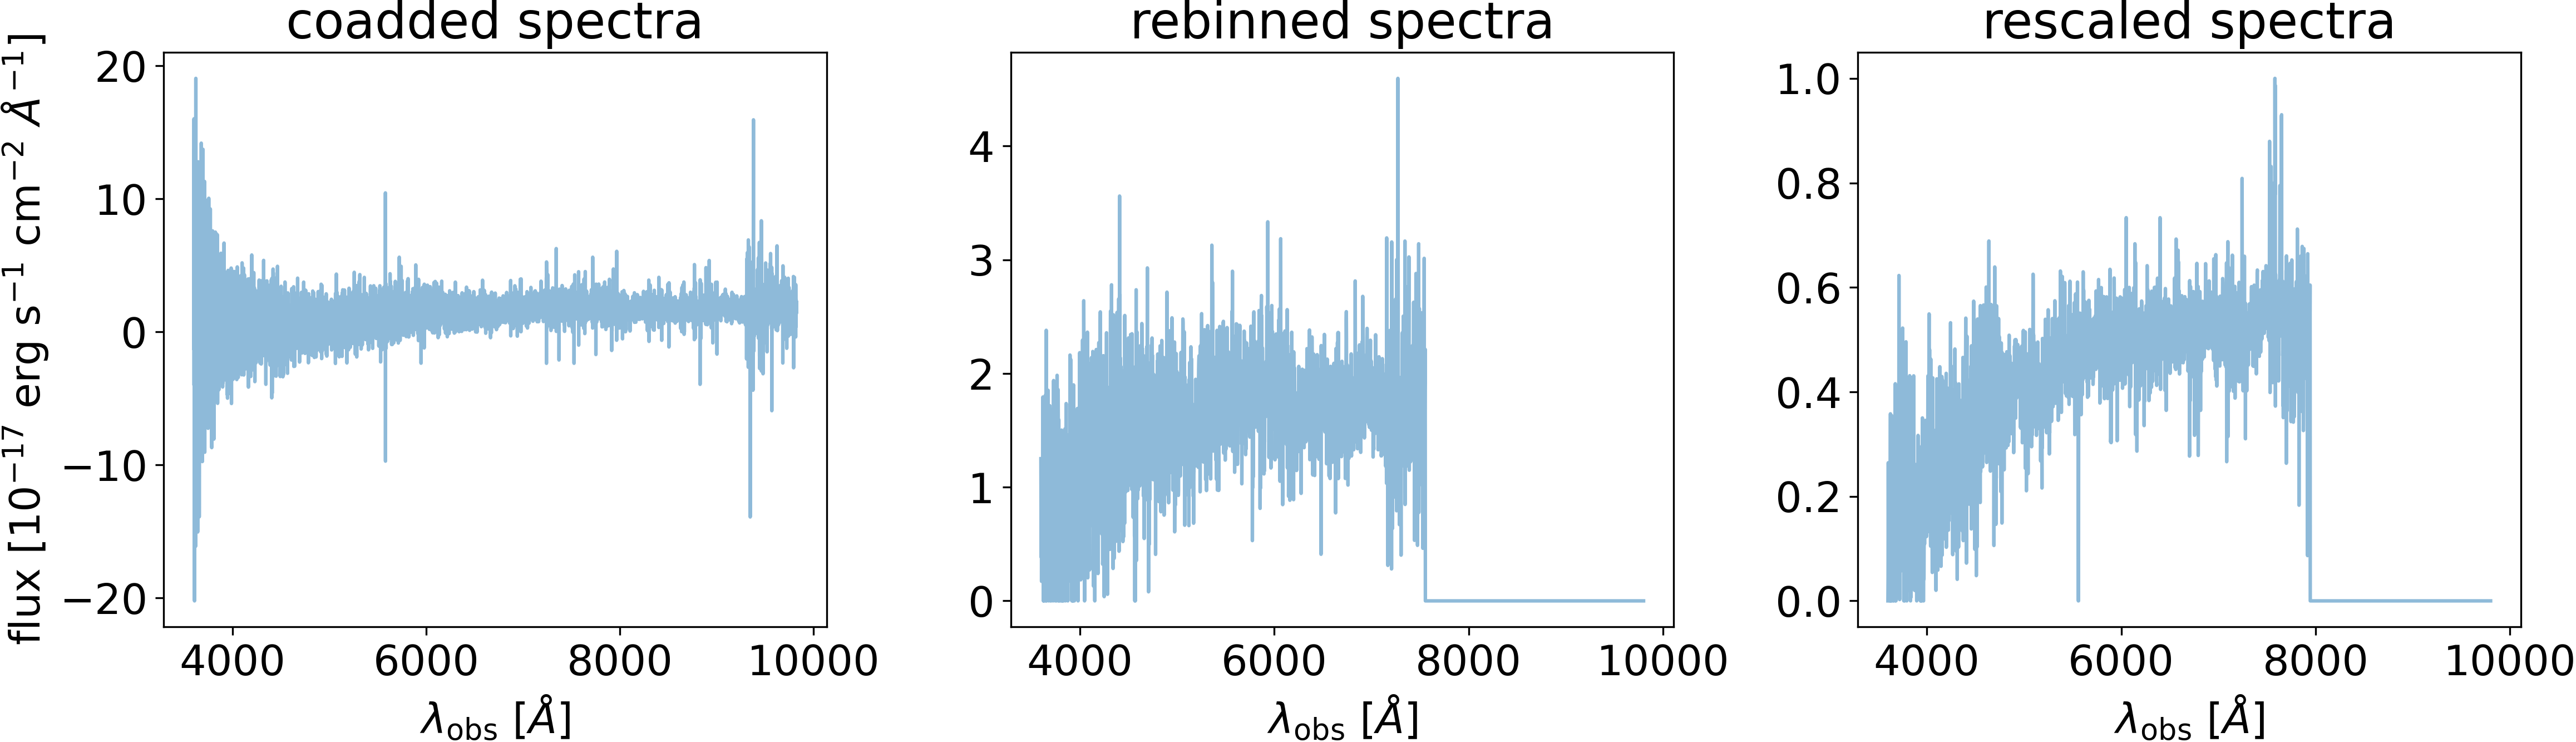
\includegraphics[width=\textwidth]{figures/preprocess/3600_Zcorrected_spectra.png}
        \caption{DESI Spectra Pre-Processing --  Redshift Corrected}
        % ]{DESI synthetic spectra undergoing pre-processing. The different bands
        % are first coadded together (left image). This is then  corrected to the galaxies rest frame and separated into 3600 
        % log-scale bins (center image). Finally, the sample is normalized between 0 and 1 (right image)}
        \label{fig:spectra_preproc}
%     \end{figure} 
% \end{frame}
%     \begin{figure}[b!]
%         \centering
        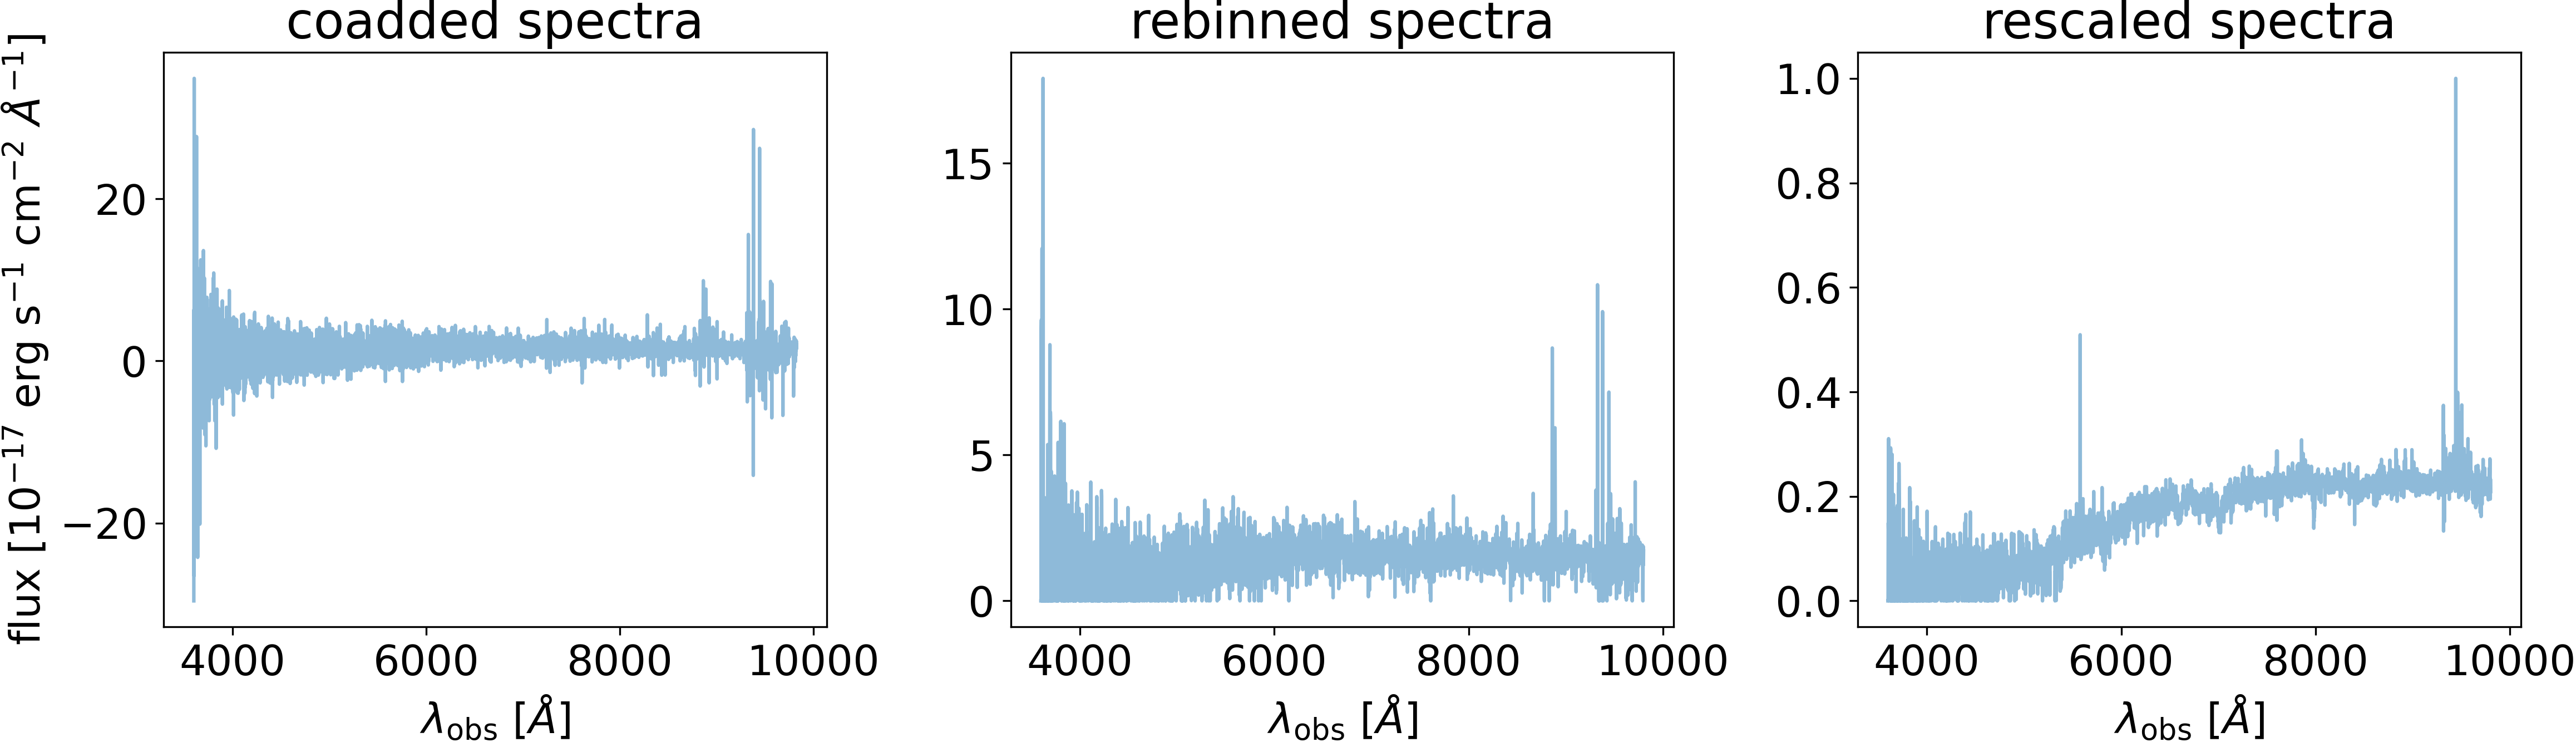
\includegraphics[width=\textwidth]{figures/preprocess/3600_Zrestframe_spectra.png}
        \caption{DESI Spectra Pre-Processing --  Non-Redshift Corrected}
        % \caption[Spectra Pre-Processing -- Not Redshift Corrected]{DESI synthetic spectra undergoing pre-processing. 
        % The different bands are first coadded together (left image). This is then separated 
        % into 3600 log-scale bins without any redshift correction (center image). Finally, 
        % the sample is normalized between 0 and 1 (right image)}
        \label{fig:sepctra_preproc_nored}
    \end{figure} 
\end{frame}

%%%%%%%%%%%%%%%%%%%%%%%%%%%%%%%%%%%%%%%%%%%%%%%%%%%%%%%%%%%%%%%%%%%%%%%%
\begin{frame}
    \begin{table}[t!]
        \small
        \centering
        \sffamily
        \begin{tabular}{lc}
	\toprule
    \textbf{Hyperparameter} & \textbf{Value} \\
    \midrule
    Learning Rate & 0.00004135238172950965 \\ 
    \midrule
    Regularization & 0.06 \\ 
    \midrule
    Dropout Rate & 0.40904759925886294\\
    \midrule
    Batch Size & 50 \\
    \bottomrule
\end{tabular}

        \caption{Hyperparameters of the CNN used to classify DESI spectra. CNN adapted 
        from \textcite{Sepeku2022}.}
        \label{tab:cnn_hyperparameters}
    \end{table}
    \begin{figure}[b!]
        \centering
        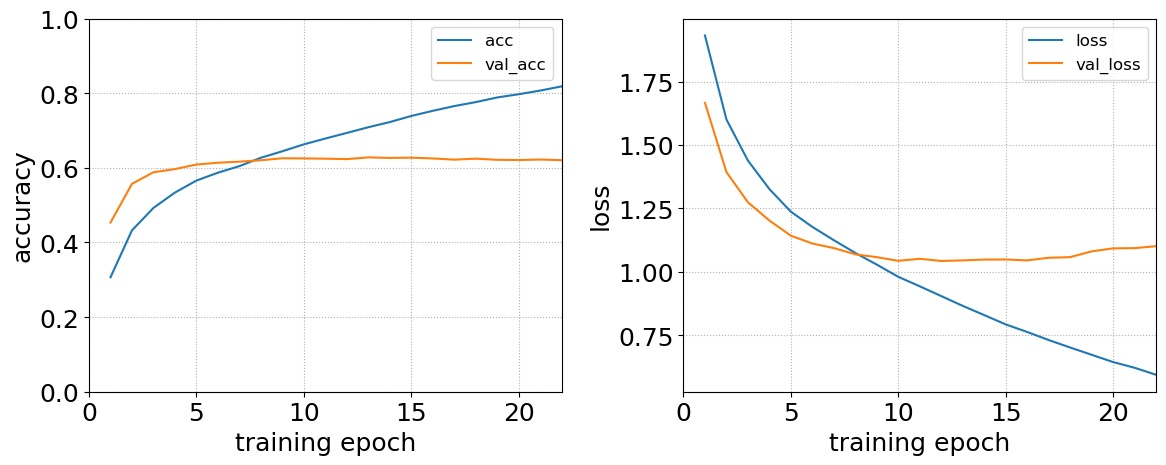
\includegraphics[width=.85\linewidth]{figures/cnn/cnn_training_history.jpg}
        \caption[CNN Training]{Training of the CNN on synthetic DESI spectra.}
        \label{fig:cnn_training}
    \end{figure}
\end{frame}


%%%%%%%%%%%%%%%%%%%%%%%%%%%%%%%%%%%%%%%%%%%%%%%%%%%%%%%%%%%%%%%%%%%%%%%%
\begin{frame}
    \begin{table}[t!]
        \small
        \centering
        \sffamily
        \begin{tabular}{lcc}
	\toprule
    \textbf{Hyperparameter} & \textbf{Smaller Architecture} & \textbf{Larger Architecture} \\
    \midrule
    Learning Rate & 0.0001 & 0.01 \\ 
    \midrule
    Batch Size & 16 & 16 \\
    \midrule
    Blocks & 4 & 4 \\
    Heads & 5 & 12 \\
    Hidden Dimension & 25 & 72 \\
    \bottomrule
\end{tabular}

        \caption{Hyperparameters of the smaller and larger Spectral ViT architecture used to classify DESI spectra.}
        \label{tab:t_hyper}
    \end{table}
    
    \begin{figure}[b!]
        \centering
        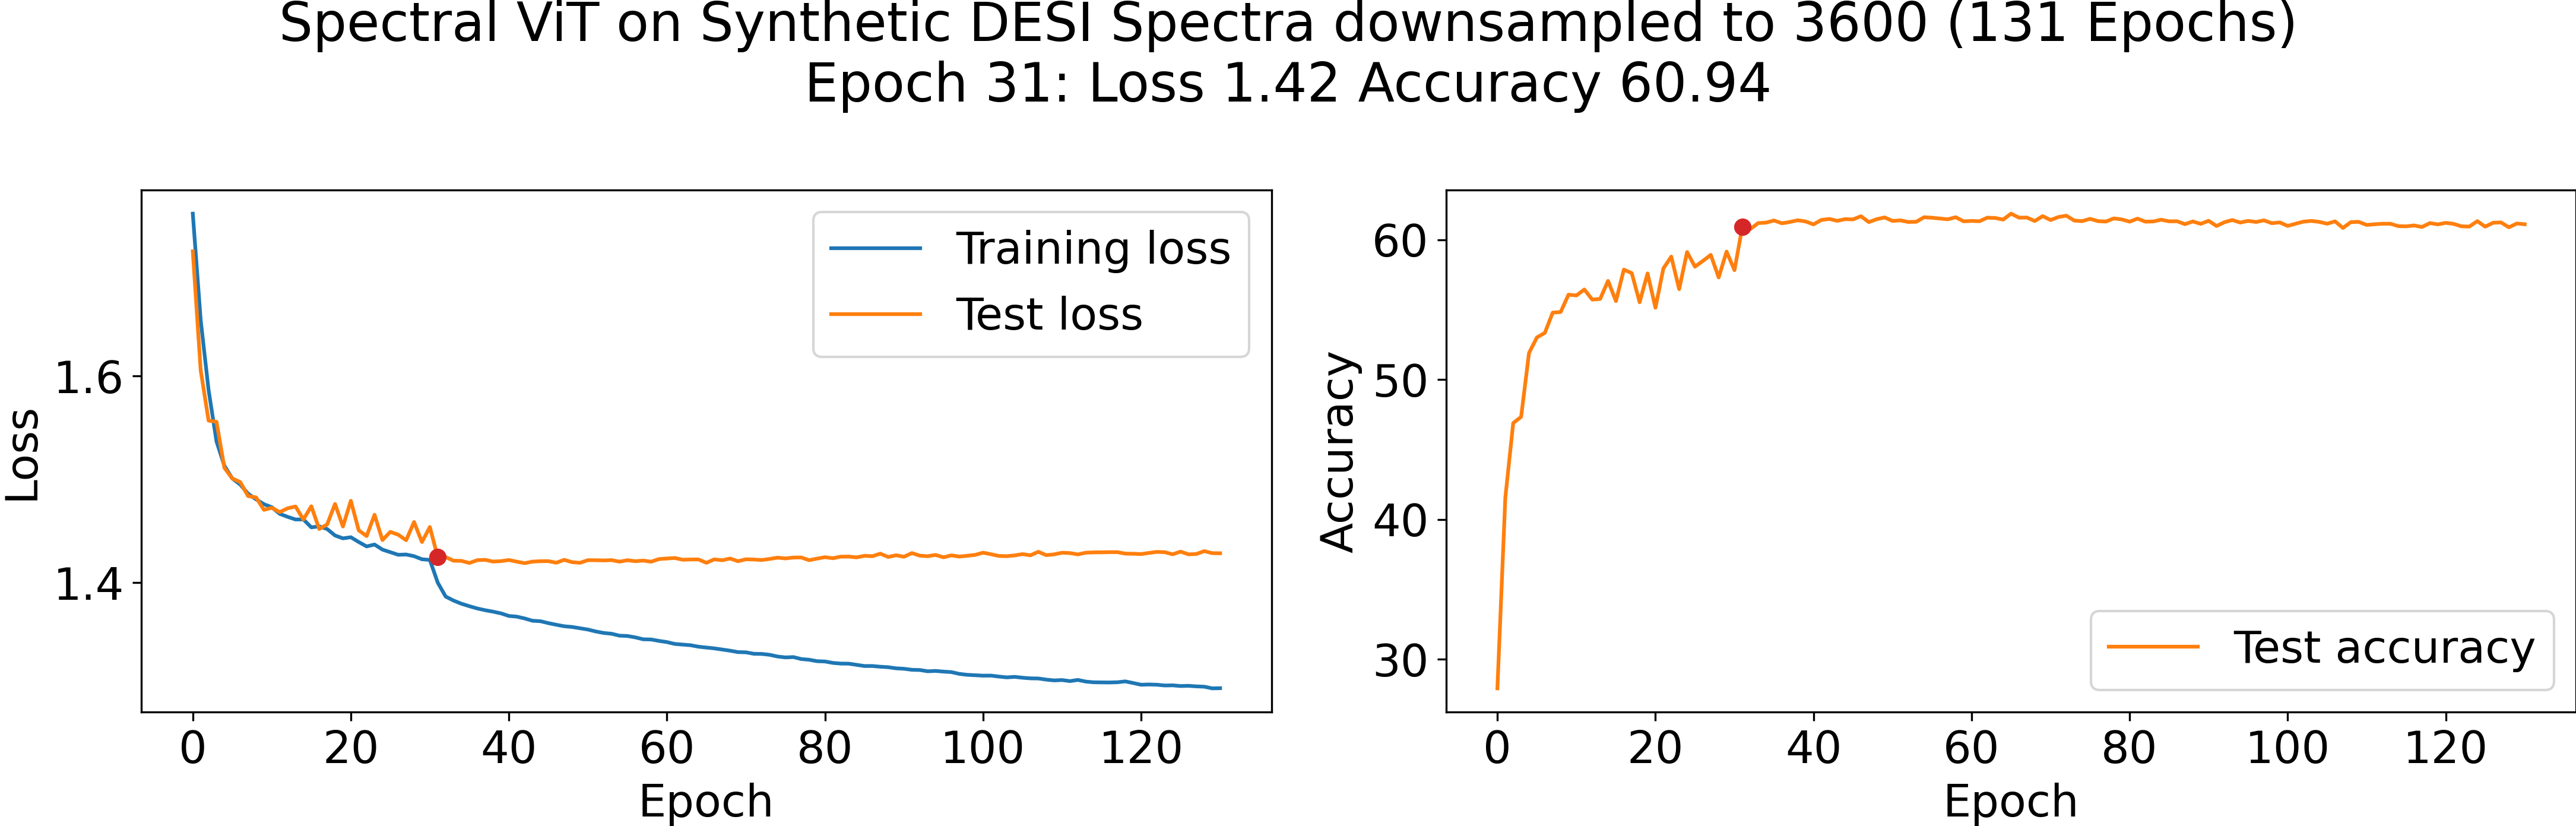
\includegraphics[width=.85\linewidth]{figures/v1_real/vit_model_V1_original_redotraining_new.png}
        \caption{Training of Spectral ViT: V1}
        % {Training of the small architecture on redshift-corrected spectra downsampled to 3600 bins. Over-fitting was determined to have occurred by Epoch 31.}
        \label{fig:vit1_training}
    \end{figure}
\end{frame}


%%%%%%%%%%%%%%%%%%%%%%%%%%%%%%%%%%%%%%%%%%%%%%%%%%%%%%%%%%%%%%%%%%%%%%%%

\begin{frame}{Additional (Failed) Training}
\centering
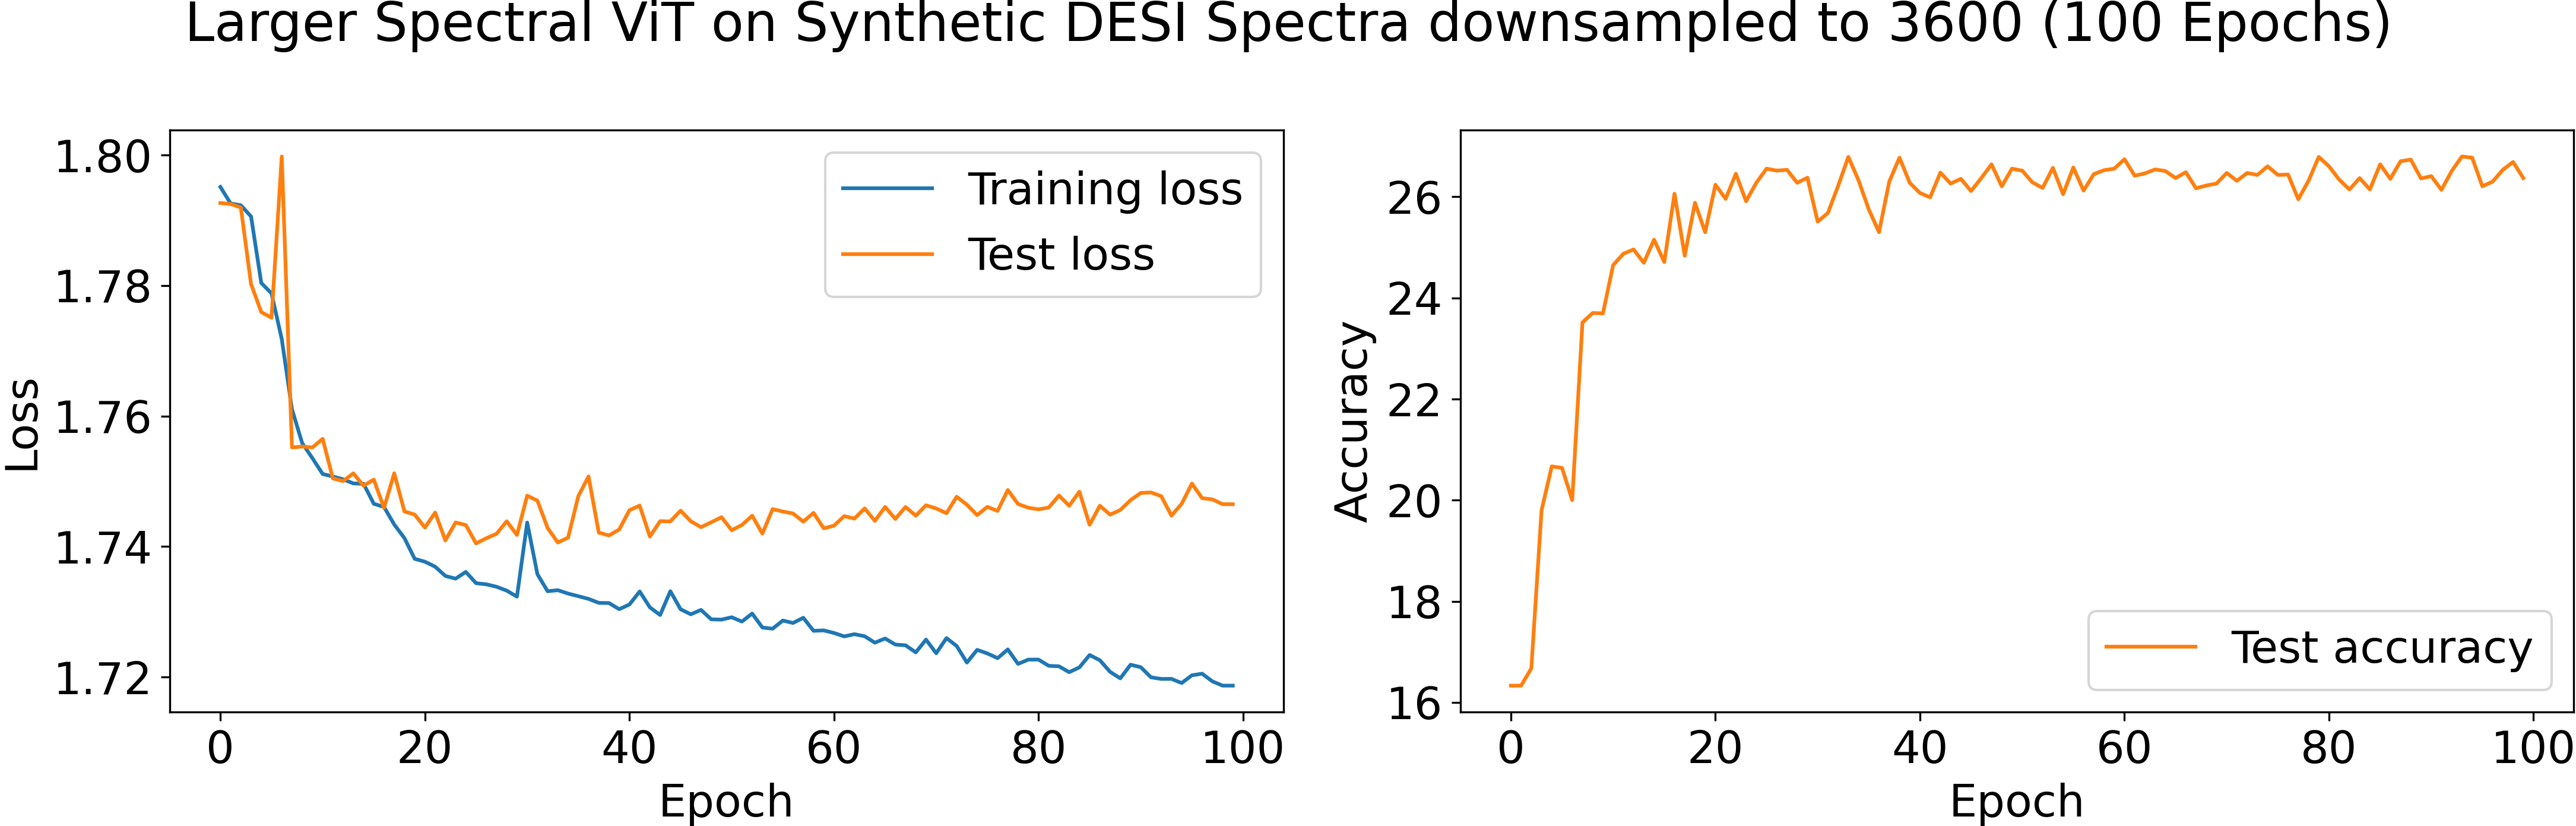
\includegraphics[width=5.5cm]{figures/v1_real/vit_model_V1_bigtraining_new.png}\\
\begin{columns}[t]
\column{.5\textwidth}
\centering
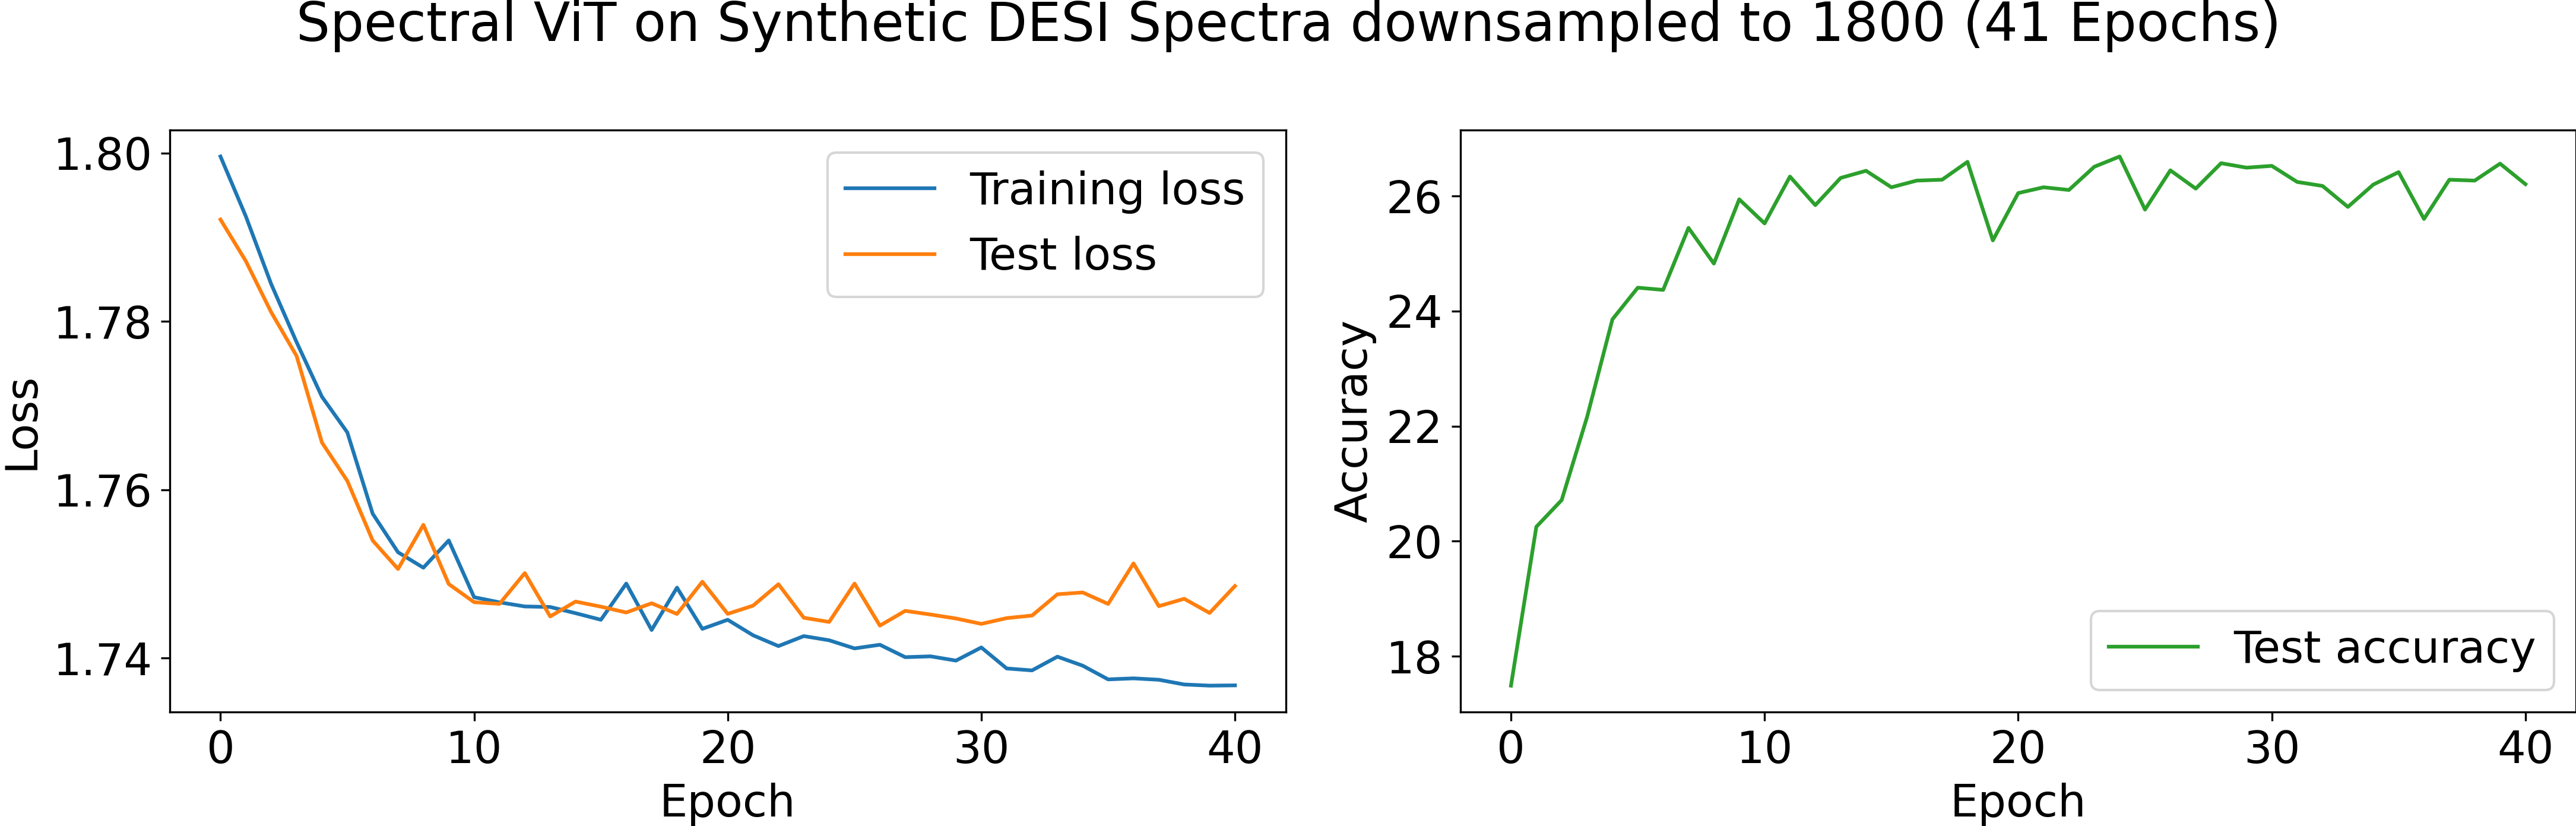
\includegraphics[width=5.5cm]{figures/vit_model_V1.2training_new.png}
\column{.5\textwidth}
\centering
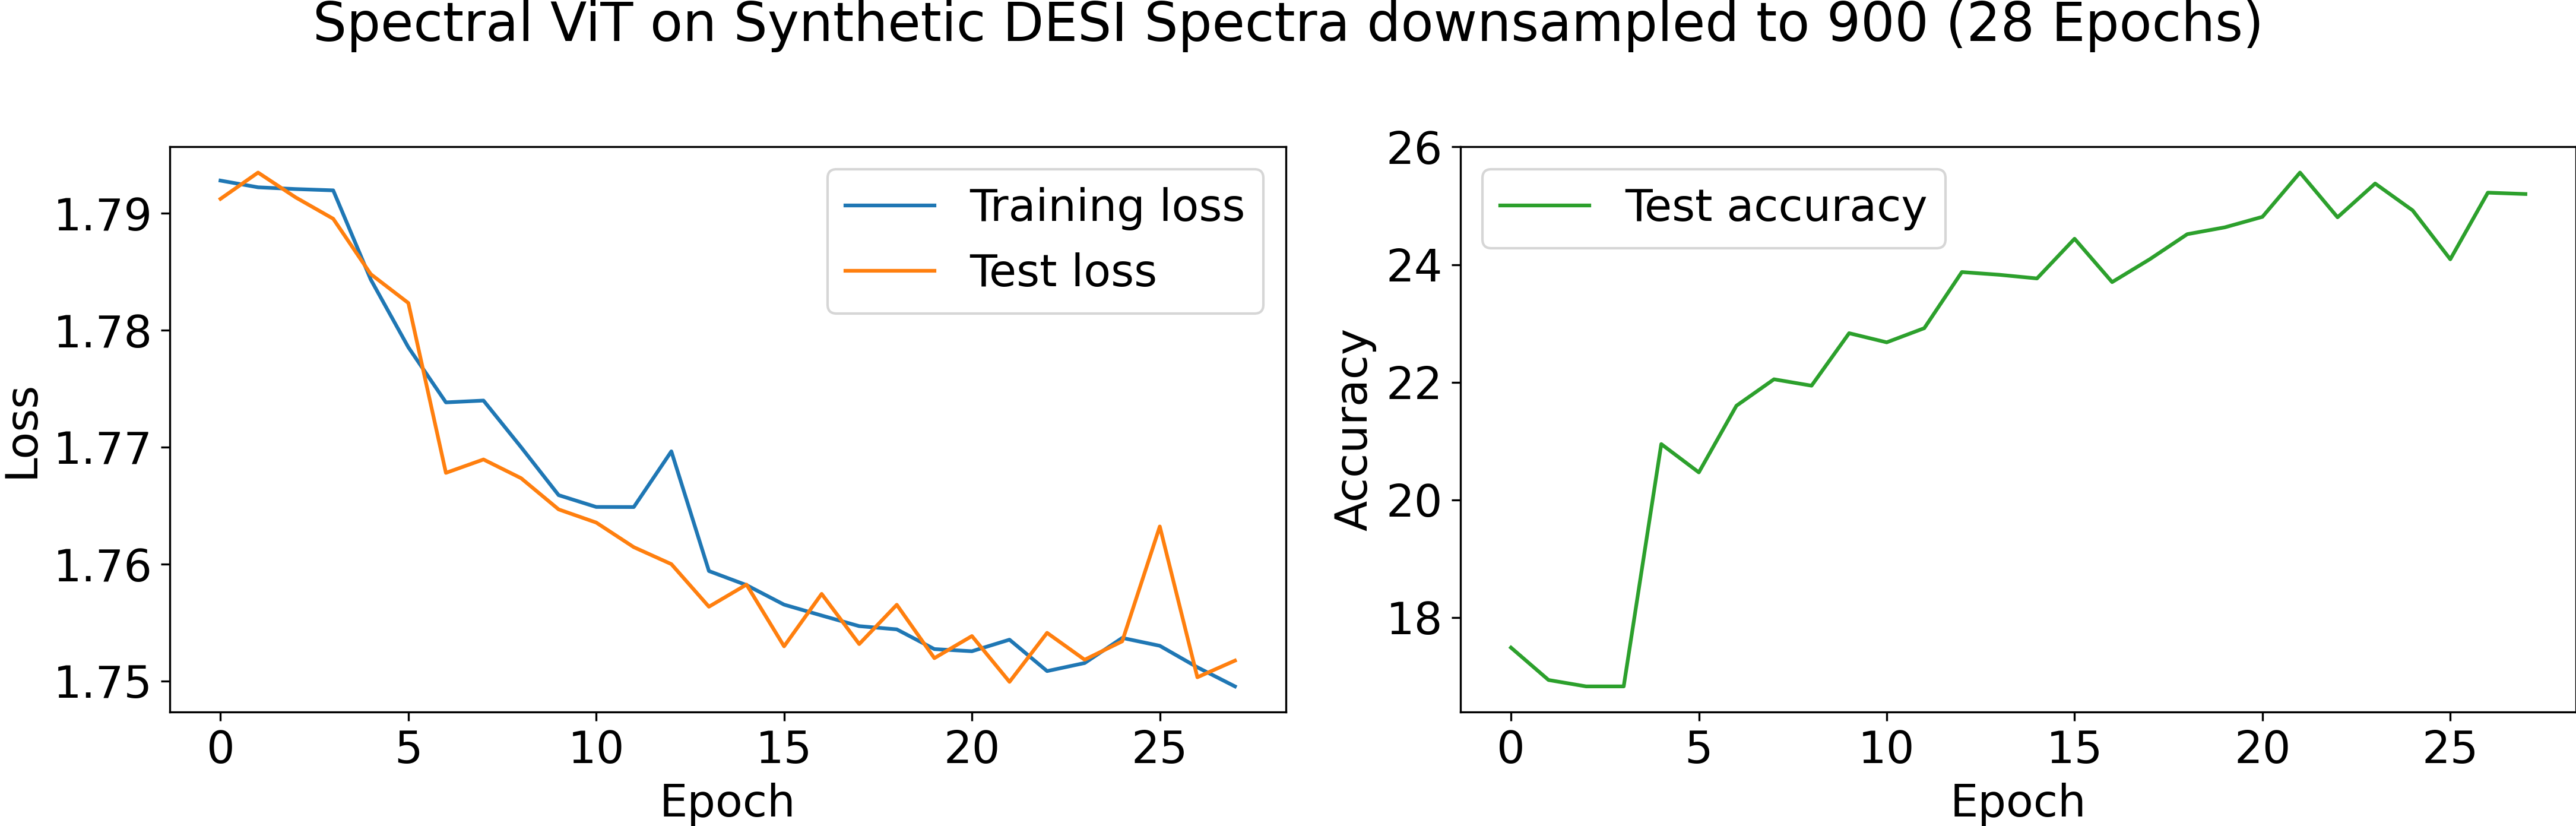
\includegraphics[width=5.5cm]{figures/vit_model_V1.3_muchsmallermodeltraining_new.png}\\
\end{columns}
\end{frame}


\begin{frame}{Training for Non-Redshift Corrected Data}
\centering
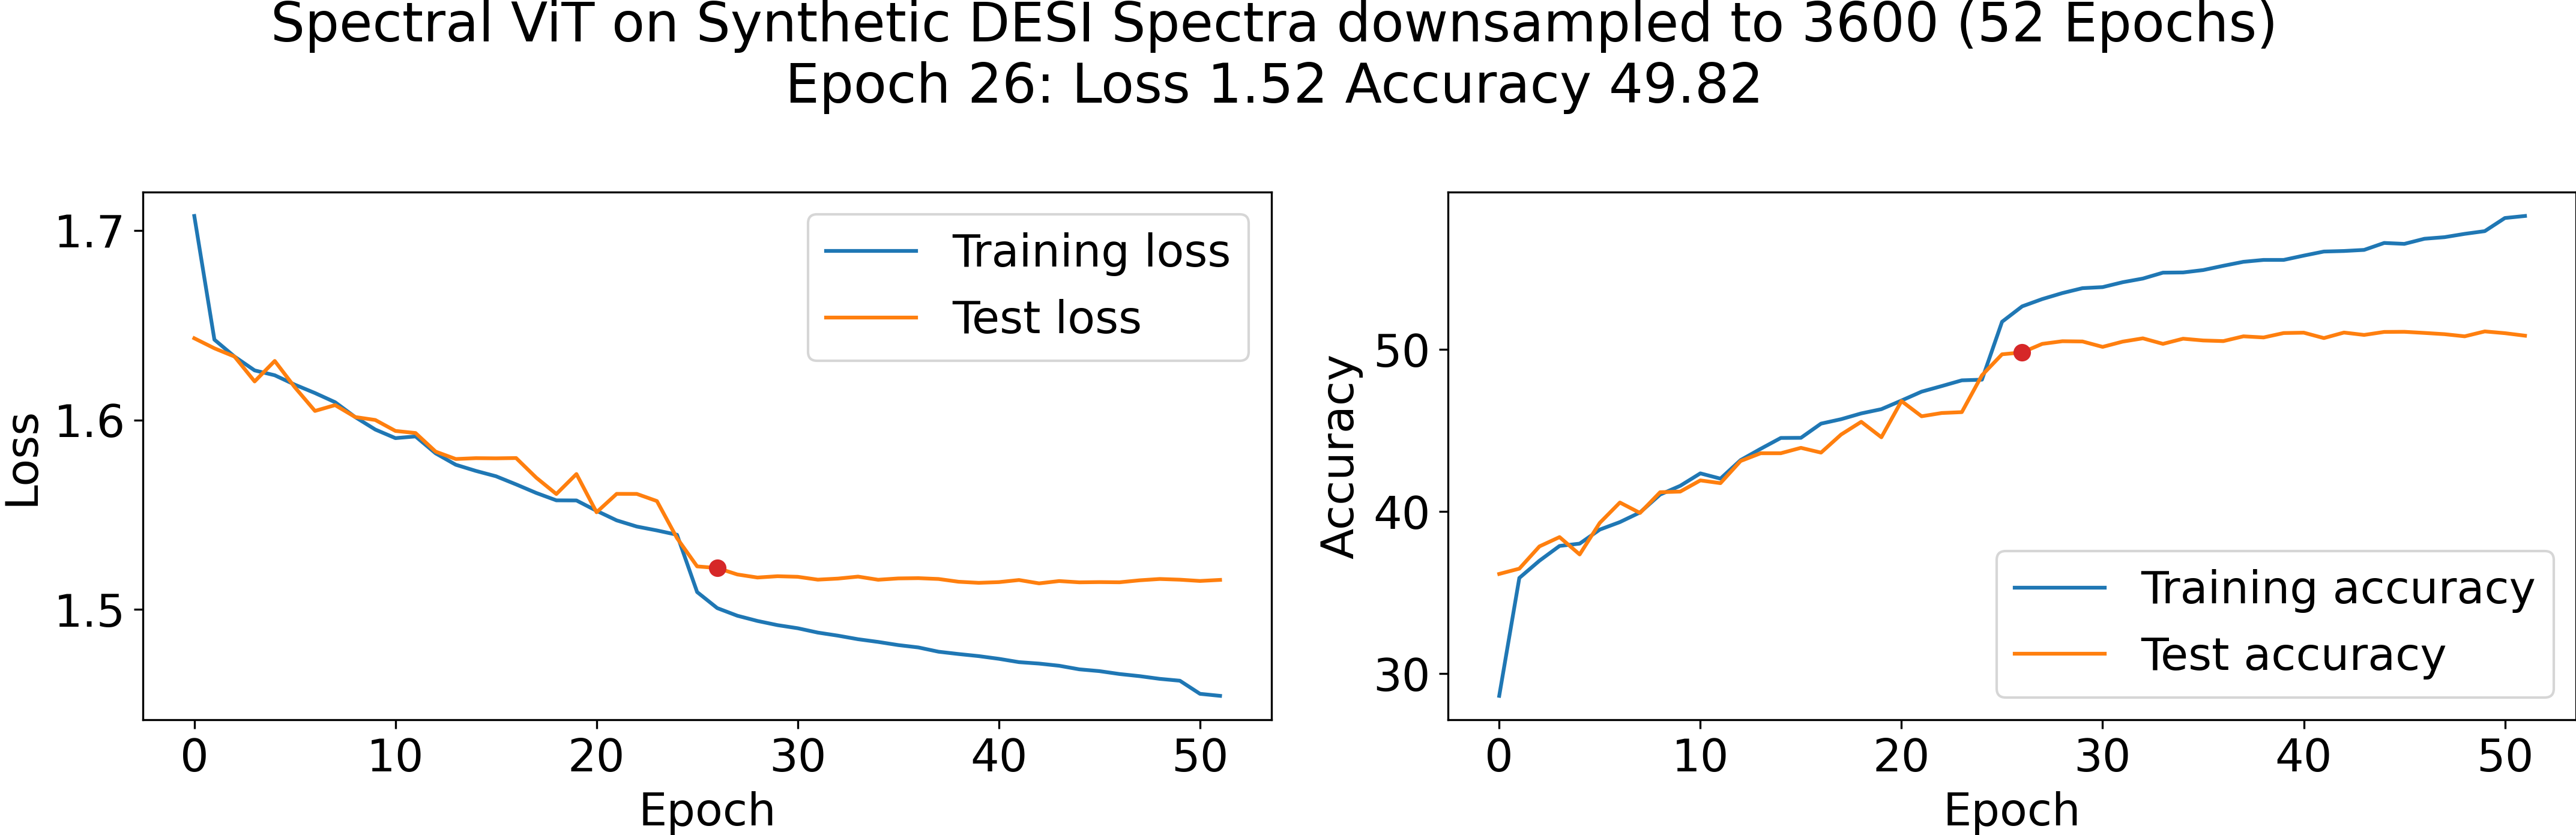
\includegraphics[width=.85\linewidth]{figures/v2_real/vit_model_V2training_new.png}
\end{frame}


\begin{comment}
%%%%%%%%%%%%%%%%%%%%%%%%%%%%%%%%%%%%%%%%%%%%%%%%%%%%%%%%%%%%%%%%%%%%%%%%
\begin{frame}
    \begin{figure}[t!]
        \centering
        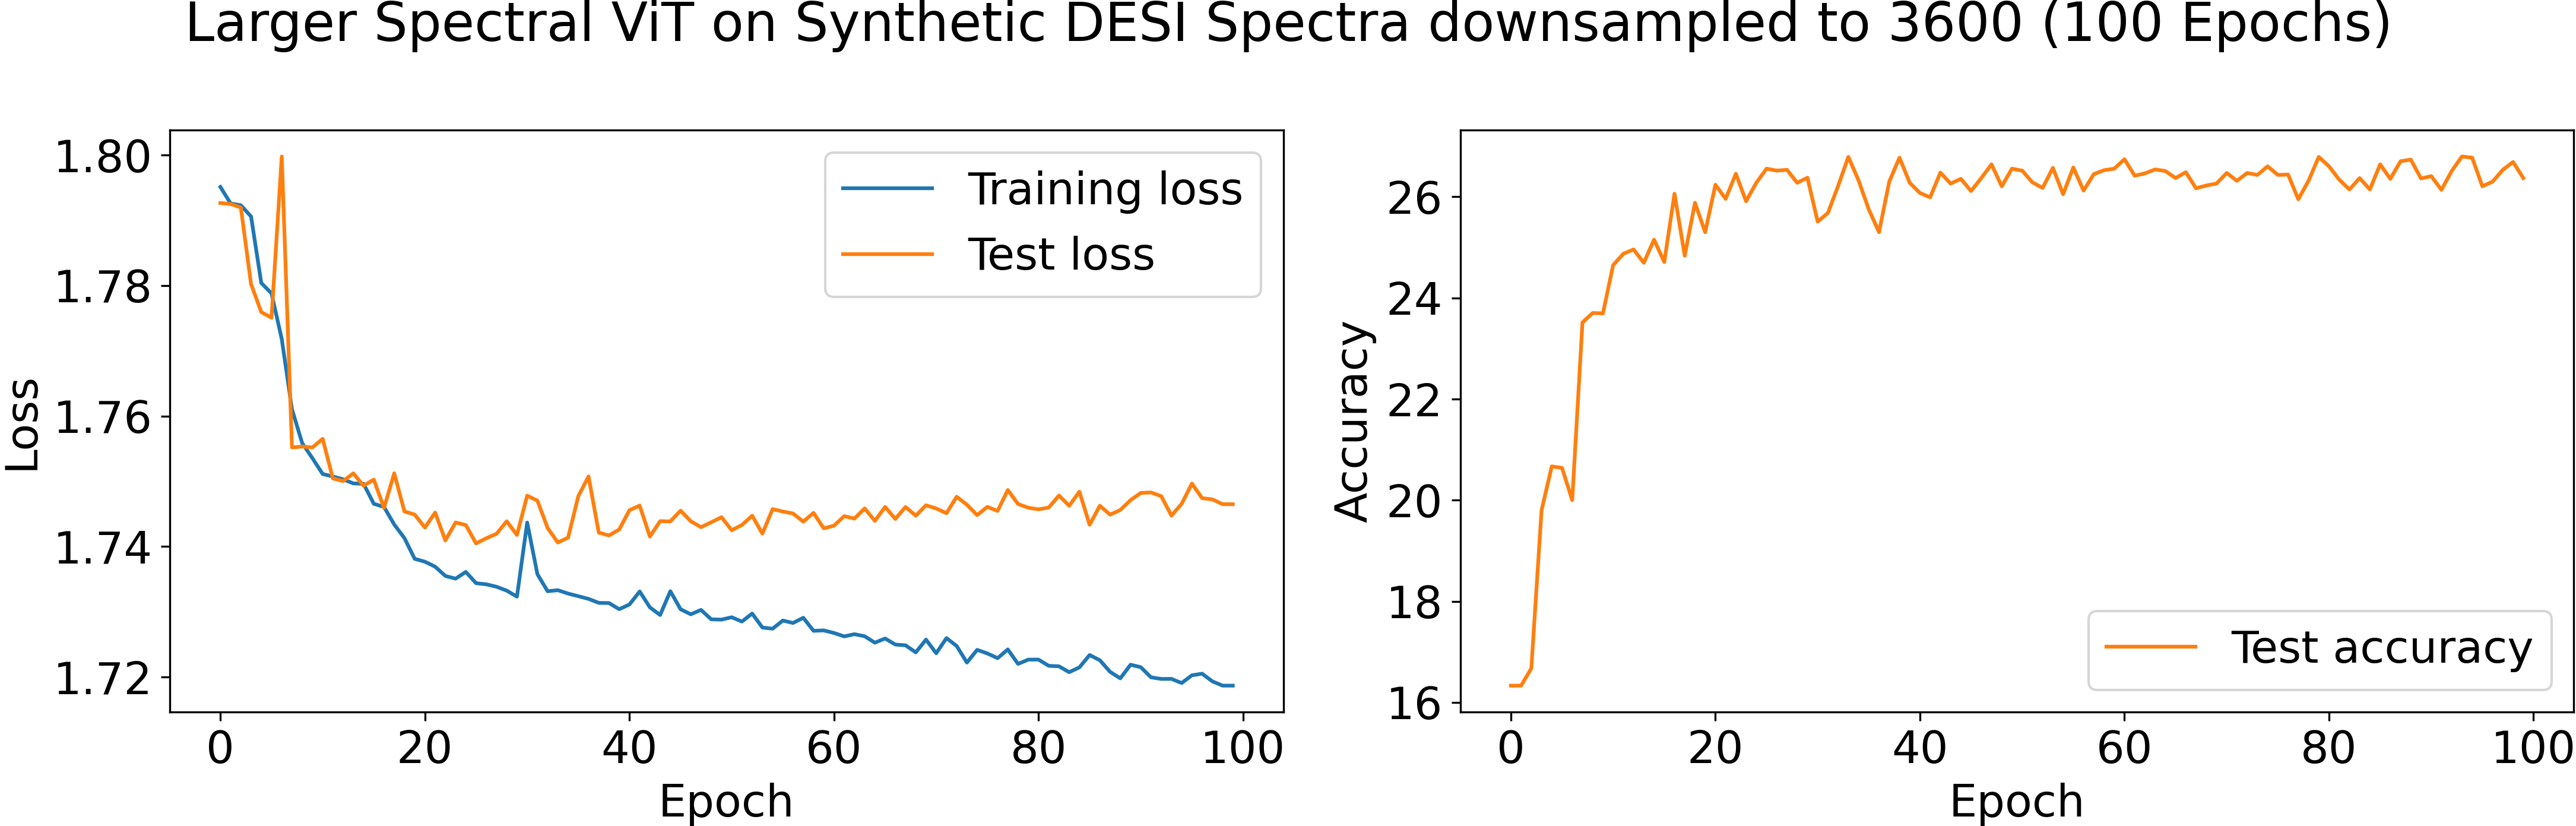
\includegraphics[width=.85\linewidth]{figures/v1_real/vit_model_V1_bigtraining_new.png}
        \caption[Training of Spectral ViT: V1 Big]{Training of the large architecture on Redshift-corrected spectra downsampled to 3600 bins. No convergence above random guessing was observed. }
        \label{fig:vit1_big_training}
    \end{figure}
\end{frame}

%%%%%%%%%%%%%%%%%%%%%%%%%%%%%%%%%%%%%%%%%%%%%%%%%%%%%%%%%%%%%%%%%%%%%%%%
\begin{frame}
    \begin{figure}[hb!]
        \centering
        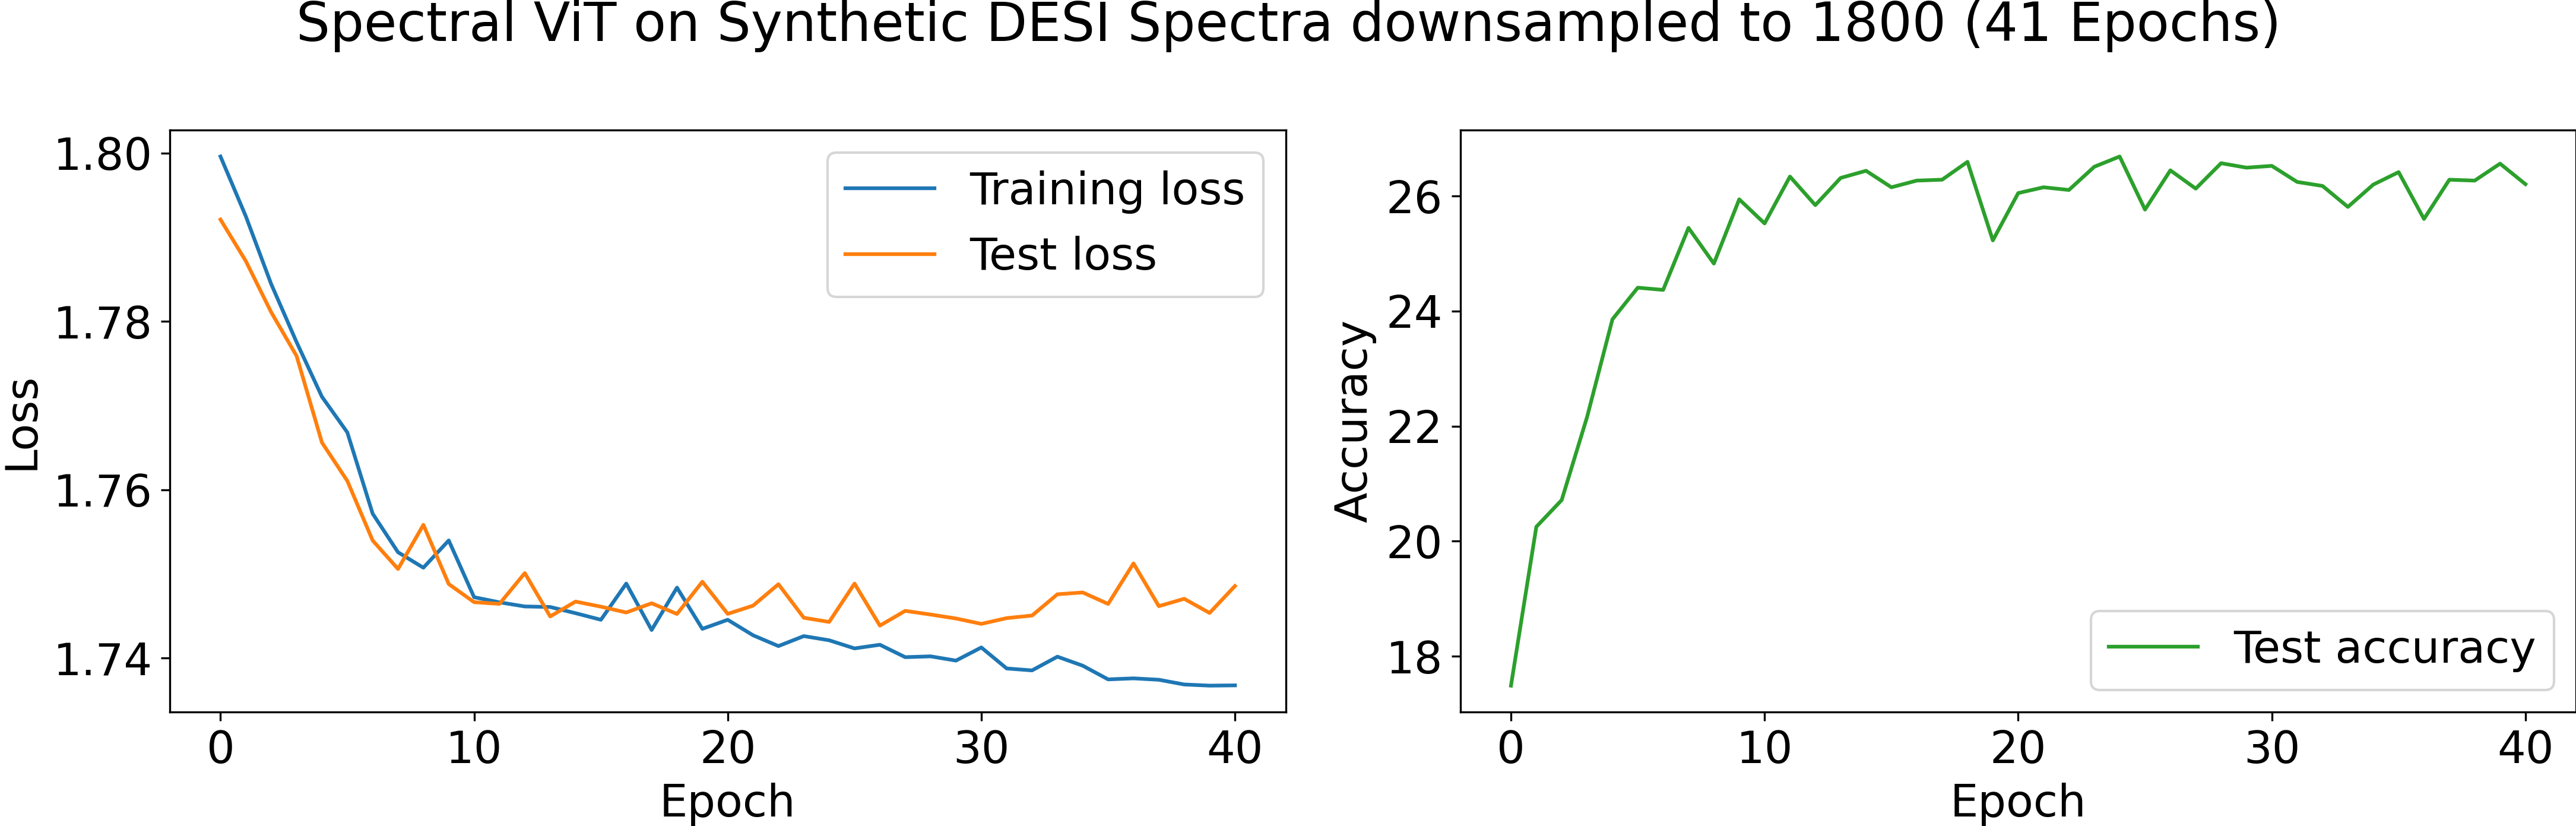
\includegraphics[width=.85\linewidth]{figures/vit_model_V1.2training_new.png}
        \caption[Training of Spectral ViT: V1.2]{Training of the small architecture on Redshift-corrected spectra downsampled to 1800 bins. No convergence above random guessing was observed. }
        \label{fig:vit1.2_training}
    \end{figure}
\end{frame}

%%%%%%%%%%%%%%%%%%%%%%%%%%%%%%%%%%%%%%%%%%%%%%%%%%%%%%%%%%%%%%%%%%%%%%%%
\begin{frame}
    \begin{figure}[t!]
        \centering
        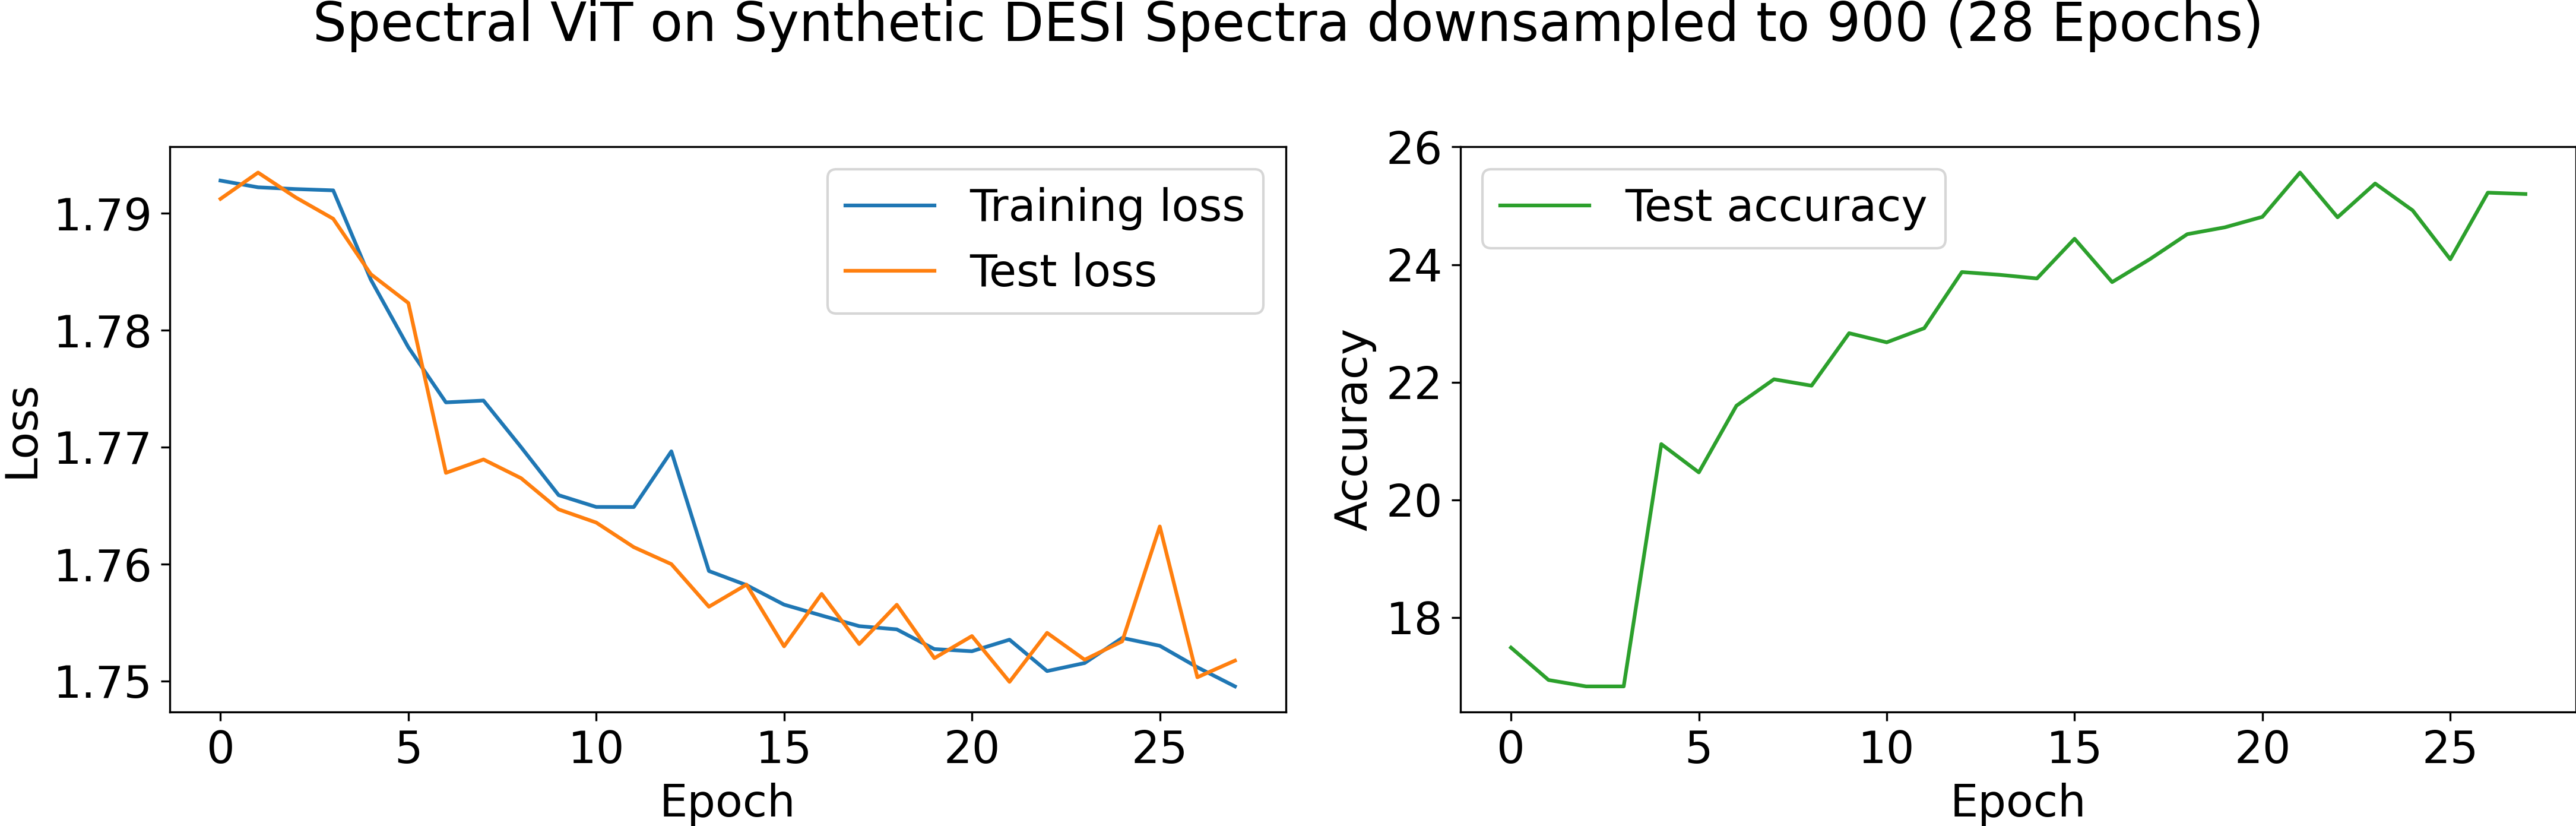
\includegraphics[width=.85\linewidth]{figures/vit_model_V1.3_muchsmallermodeltraining_new.png}
        \caption[Training of Spectral ViT: V1.3]{Training of the small architecture on Redshift-corrected spectra downsampled to 900 bins. No convergence above random guessing was observed. }
        \label{fig:vit1.3_training}
    \end{figure}
\end{frame}


%%%%%%%%%%%%%%%%%%%%%%%%%%%%%%%%%%%%%%%%%%%%%%%%%%%%%%%%%%%%%%%%%%%%%%%%
\begin{frame}
    \begin{figure}[t!]
        \centering
        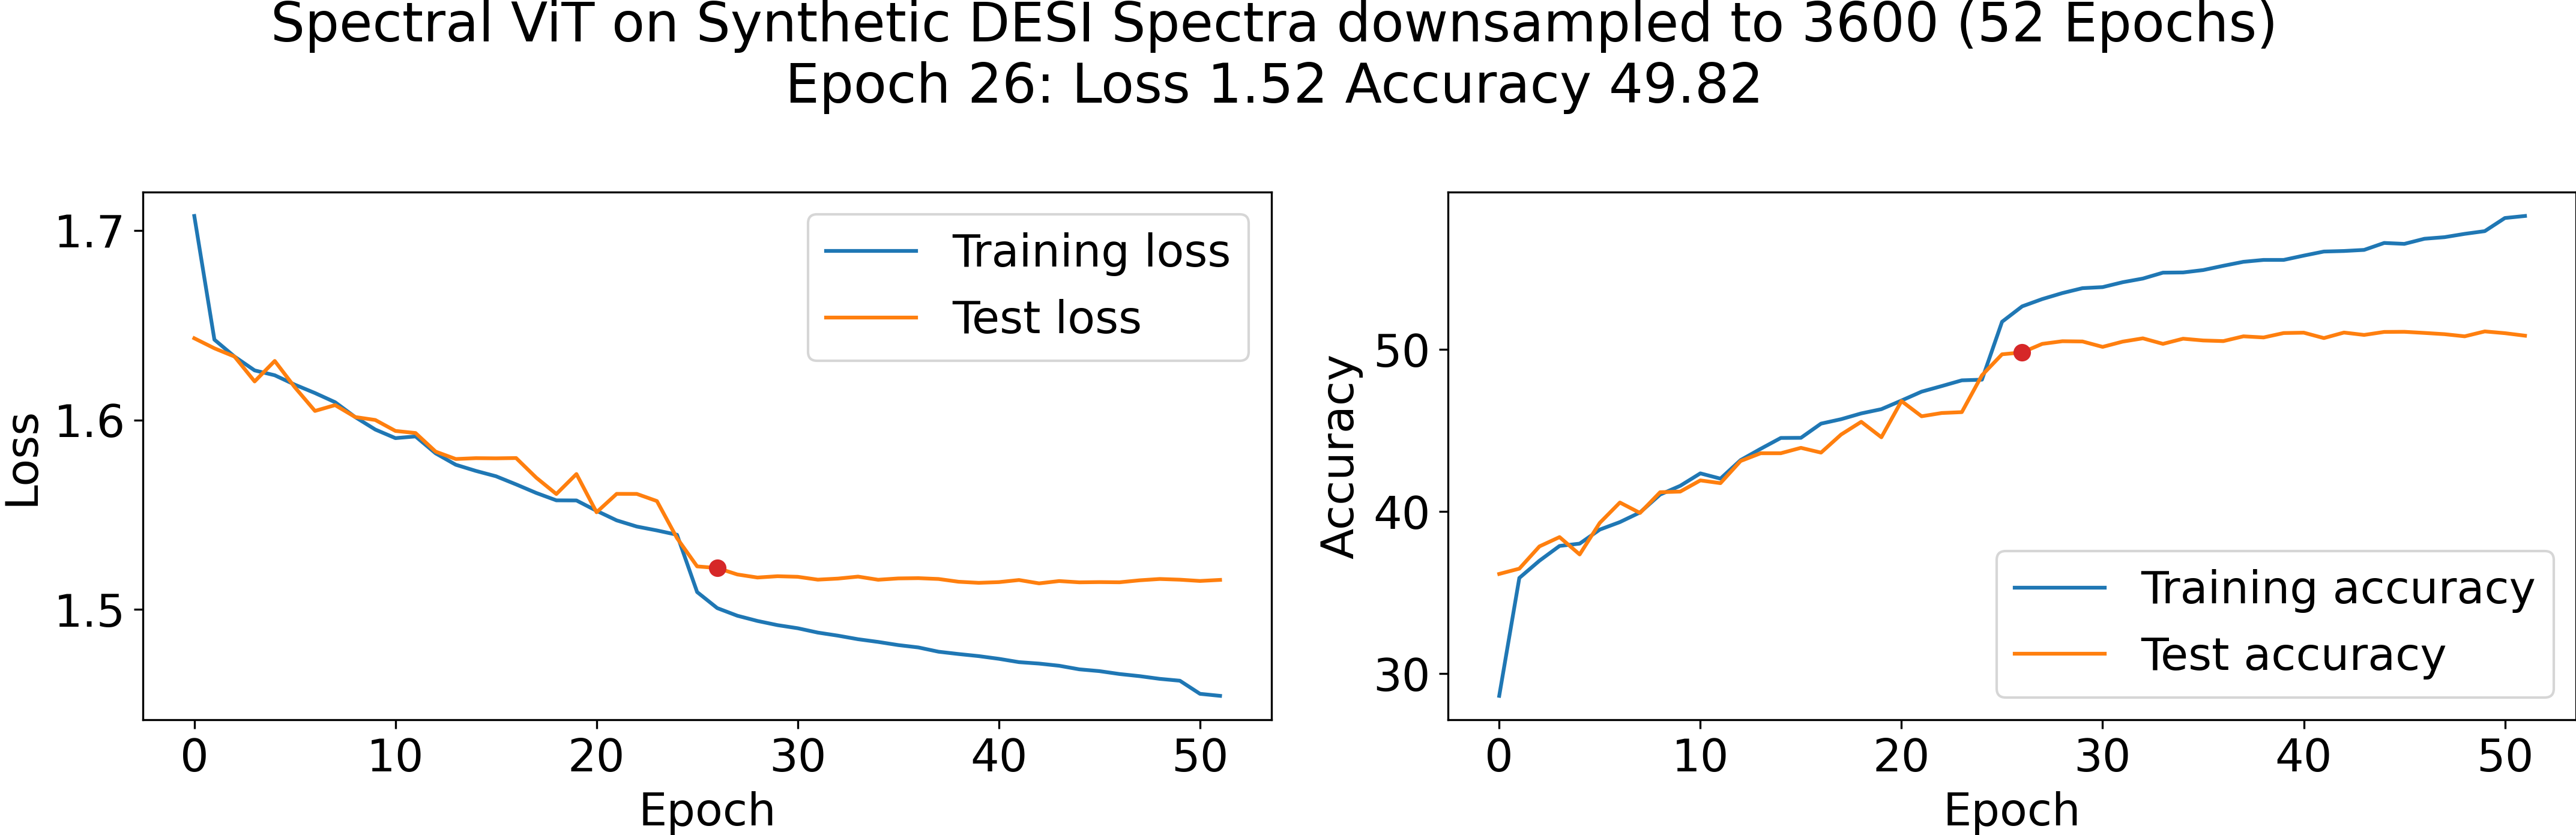
\includegraphics[width=.85\linewidth]{figures/v2_real/vit_model_V2training_new.png}
        \caption[Training of Spectral ViT: V2]{Training of the small architecture on non Redshift-corrected data downsampled to 3600 bins. Over fitting was determined to have occurred by Epoch 26.}
        \label{fig:vit2_training}
    \end{figure}
\end{frame}
\end{comment}




\begin{comment}
%%%%%%%%%%%%%%%%%%%%%%%%%%%%%%%%%%%%%%%%%%%%%%%%%%%%%%%%%%%%%%%%%%%%%%%%
\begin{frame}
    \frametitle{Training}
    \small
    \begin{table}
        \centering
        \caption{HAM10000 Dataset Split}
        \resizebox{\linewidth}{!}{\begin{tabular}{lccc}
	\toprule
    \textbf{Spam} & \textbf{Ni} & \textbf{Swallow} & \textbf{Shrubbery} \\
    \midrule
    A & 1 & 2 & 3 \\
    \midrule
    E & 3 & 4 & 5 \\
    C & 6 & 9 & 3 \\
    \midrule
    M & 4 & 1 & 1 \\
    \bottomrule
\end{tabular}}
    \end{table}
\end{frame}
%%%%%%%%%%%%%%%%%%%%%%%%%%%%%%%%%%%%%%%%%%%%%%%%%%%%%%%%%%%%%%%%%%%%%%%%
\begin{frame}[fragile]
    \frametitle{Verification of Model}
    \begin{block}{Classification}
        Does the predicted class match the true class? 
    \end{block}
    \begin{block}{Segmentation}
    First take the softmax of the outputs (limit from 0 to 1), then compare to true mask
    \begin{exampleblock}{Dice Score}
        \begin{equation}\label{eqn:DiceScore}
            \text{Dice} = \frac{2|X \cap Y|}{|X| + |Y| + \epsilon}
        \end{equation}
        Where $\epsilon$ is a small constant to prevent division by 0. 
    \end{exampleblock}
    
    \end{block}

\end{frame}
\end{comment}

%%%%%%%%%%%%%%%%%%%%%%%%%%%%%%%%%%%%%%%%%%%%%%%%%%%%%%%%%%%%%%%%%%%%%%%%

\section[Model Performance]{Spectral ViT Model Performance}
\begin{frame}{Spectral ViT V1}
    \begin{figure}
        \centering
        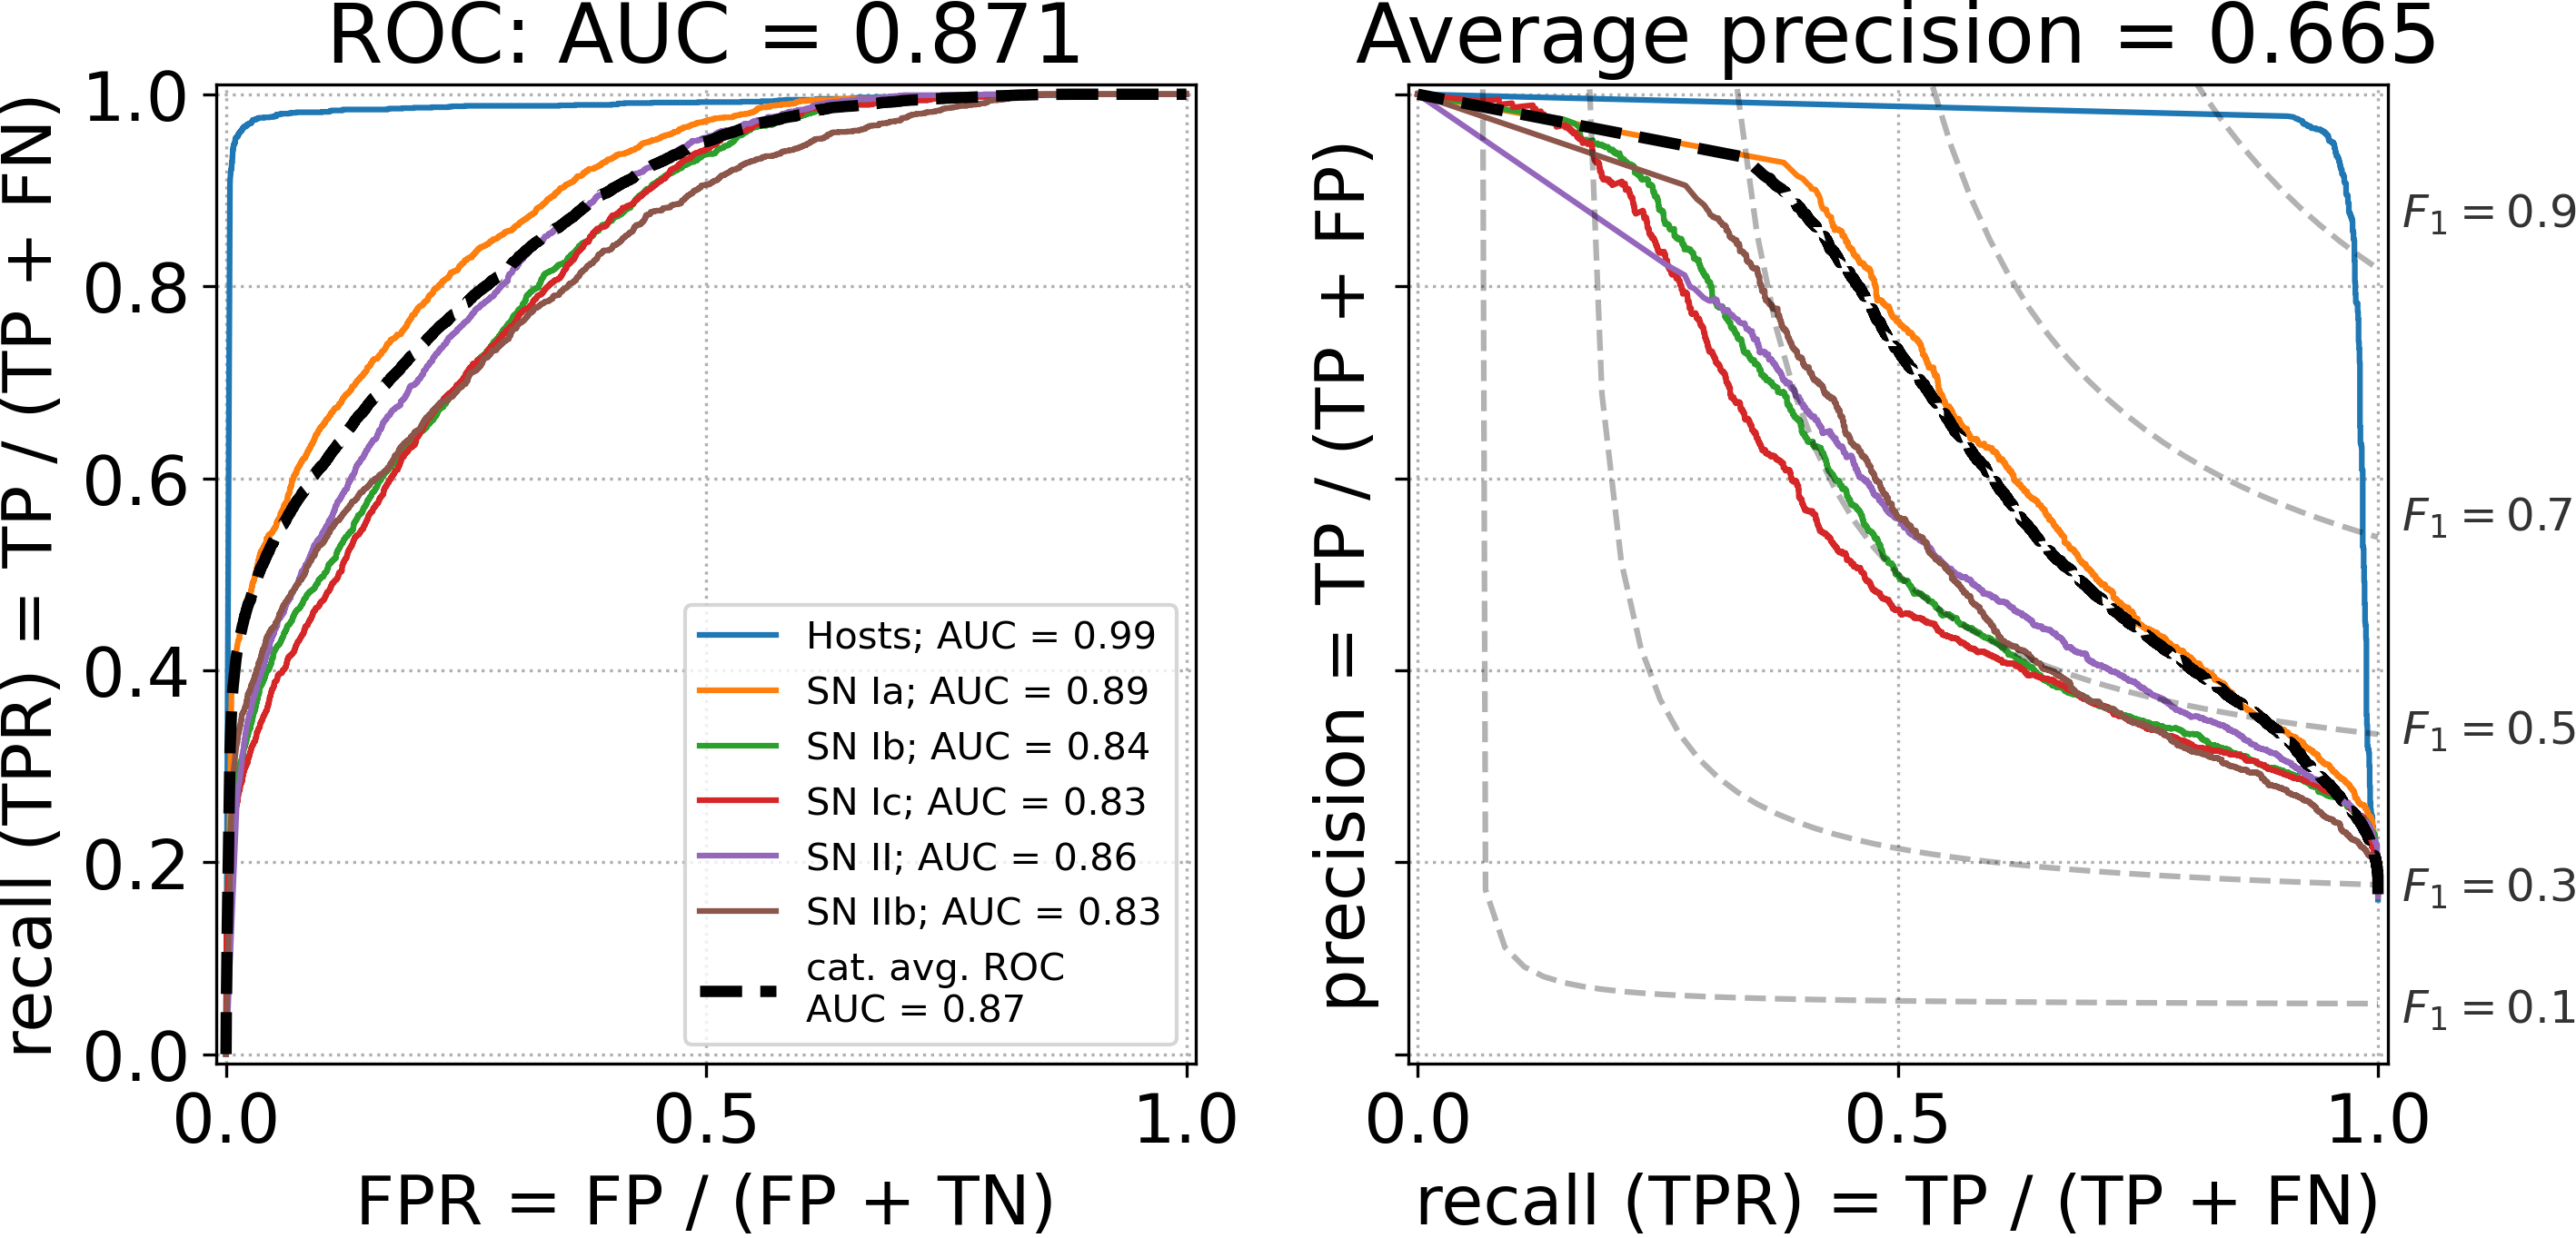
\includegraphics[height=2.8cm]{figures/v1_real/vit_model_V1_original_redorocfulle_e31.png}
        \quad
        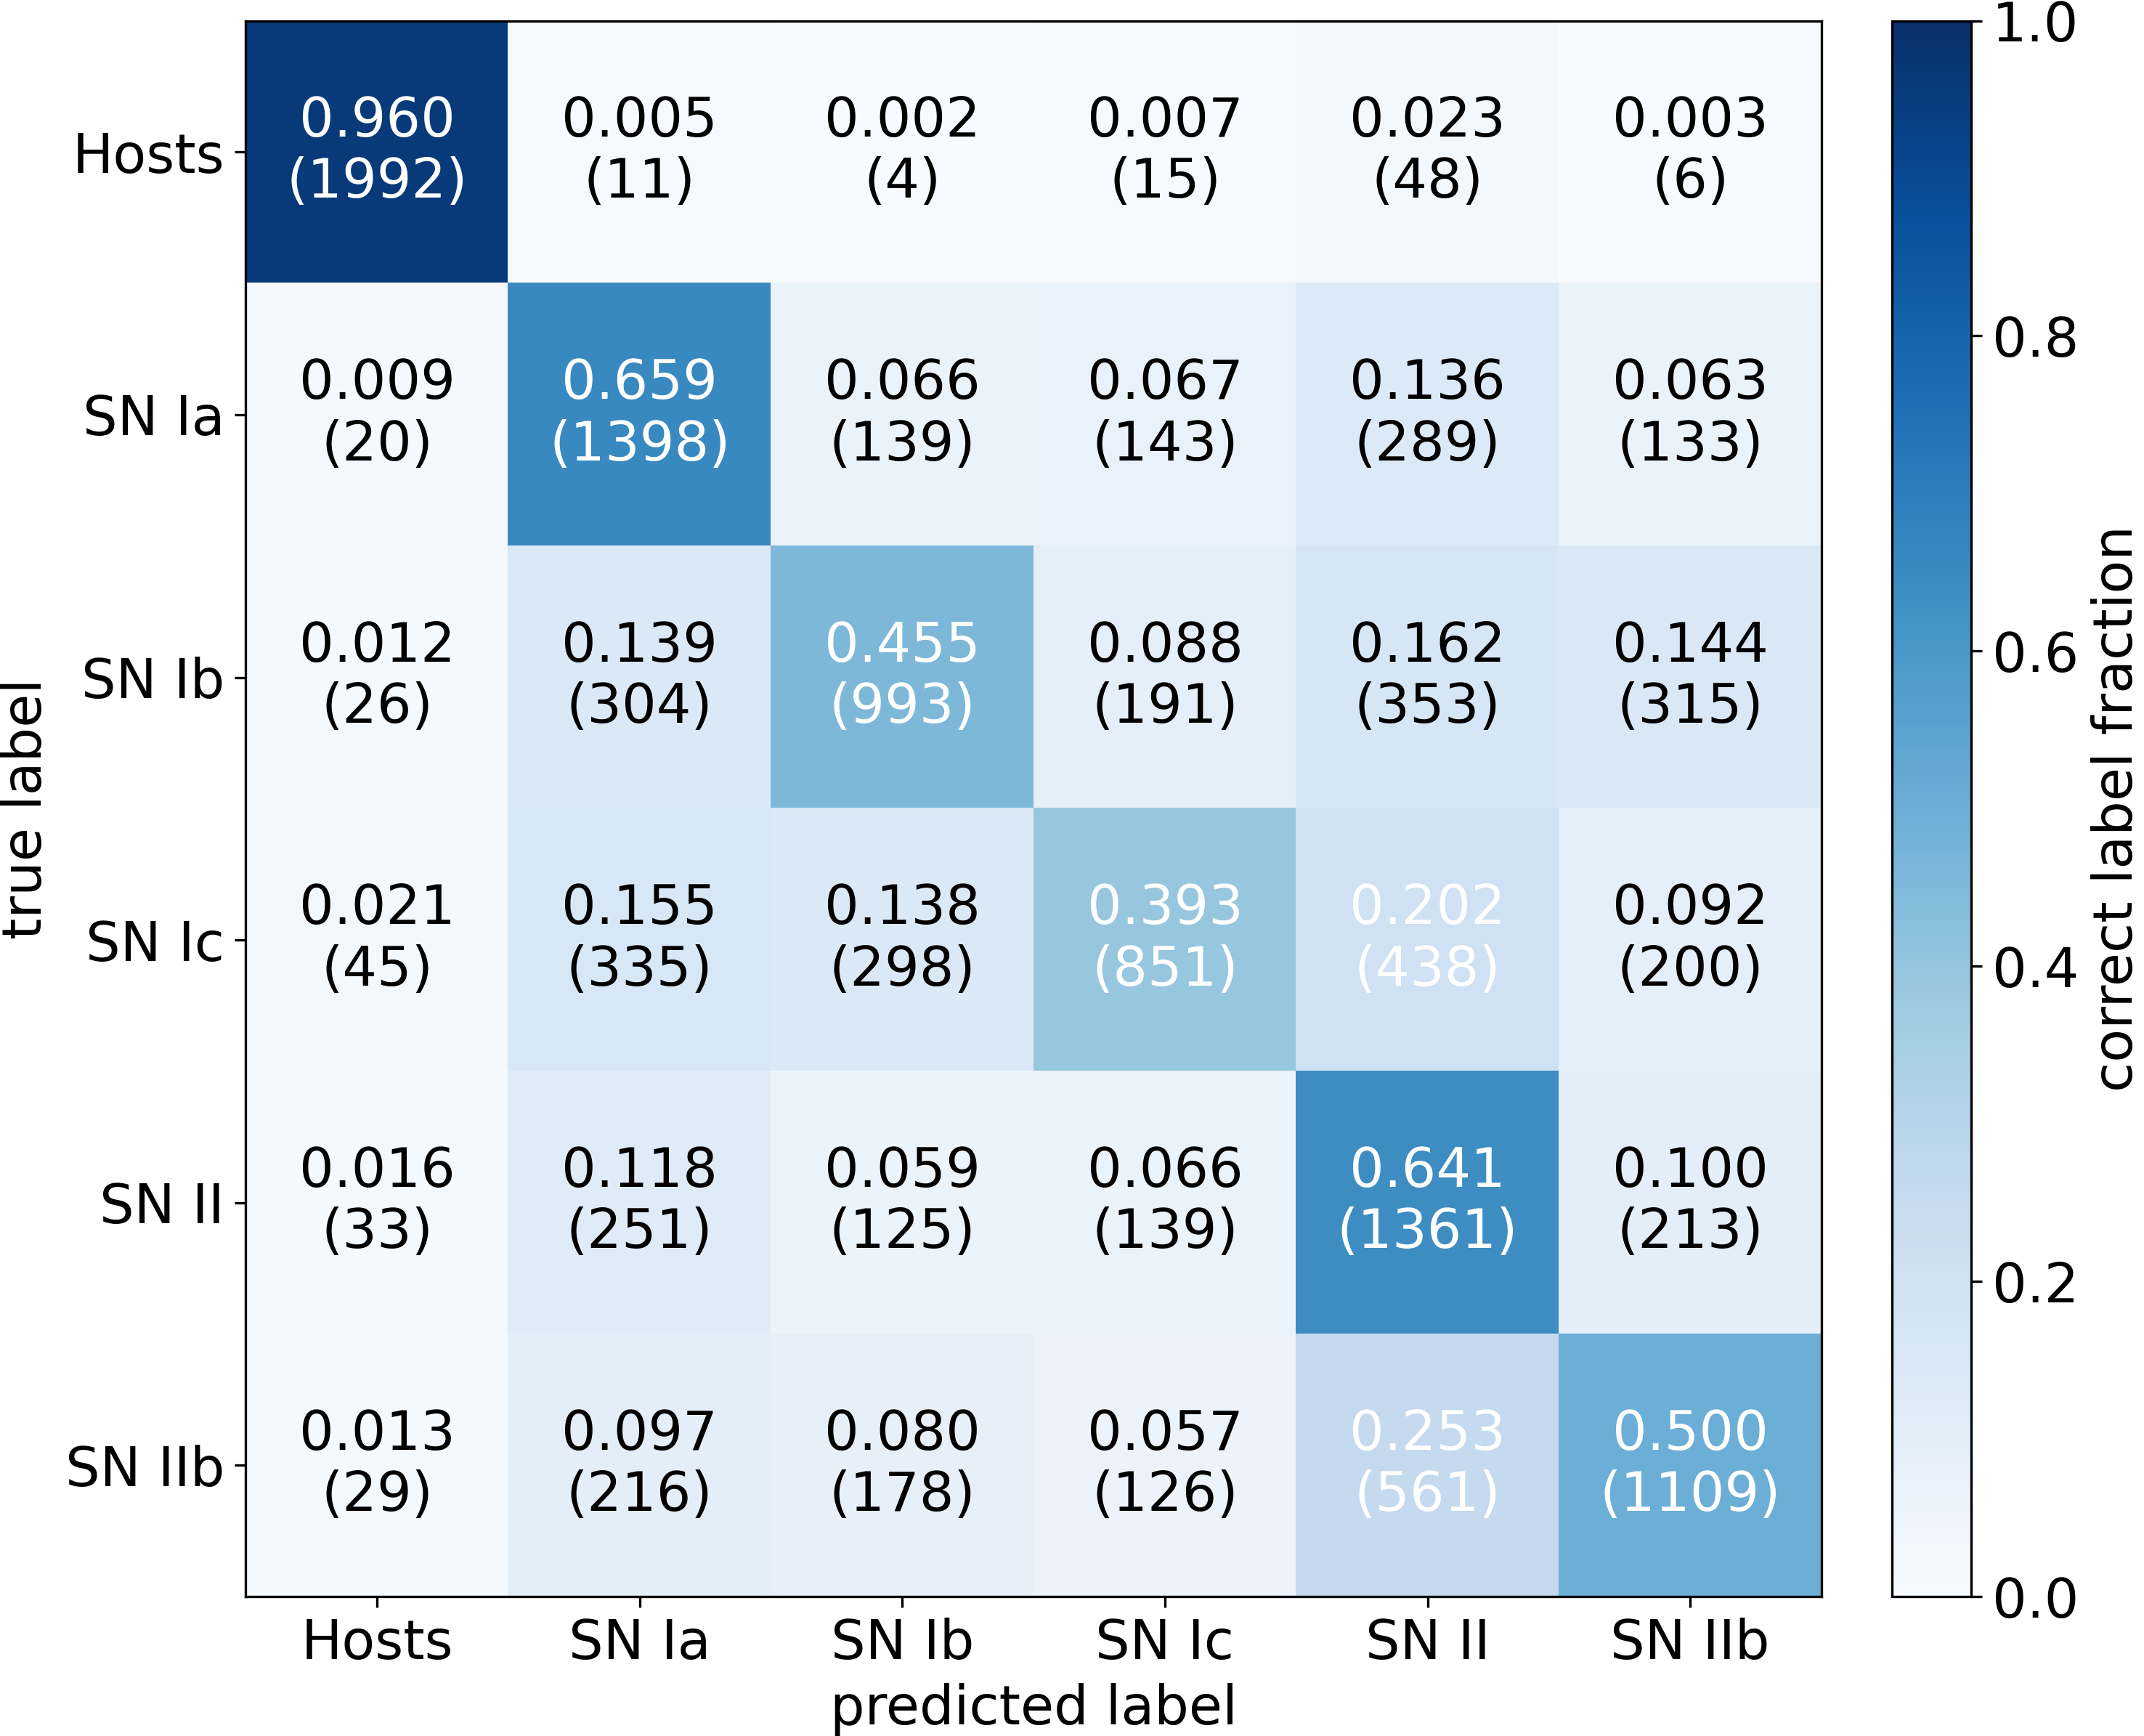
\includegraphics[height=2.8cm]{figures/v1_real/vit_model_V1_original_redocmfull_e31.png}
        \caption{Spectral ViT V1 Classifier\label{fig:v1_qual}}
        \pause
%     \end{figure}
% \end{frame}

% \begin{frame}
%     \begin{figure}[t]
%         \centering
        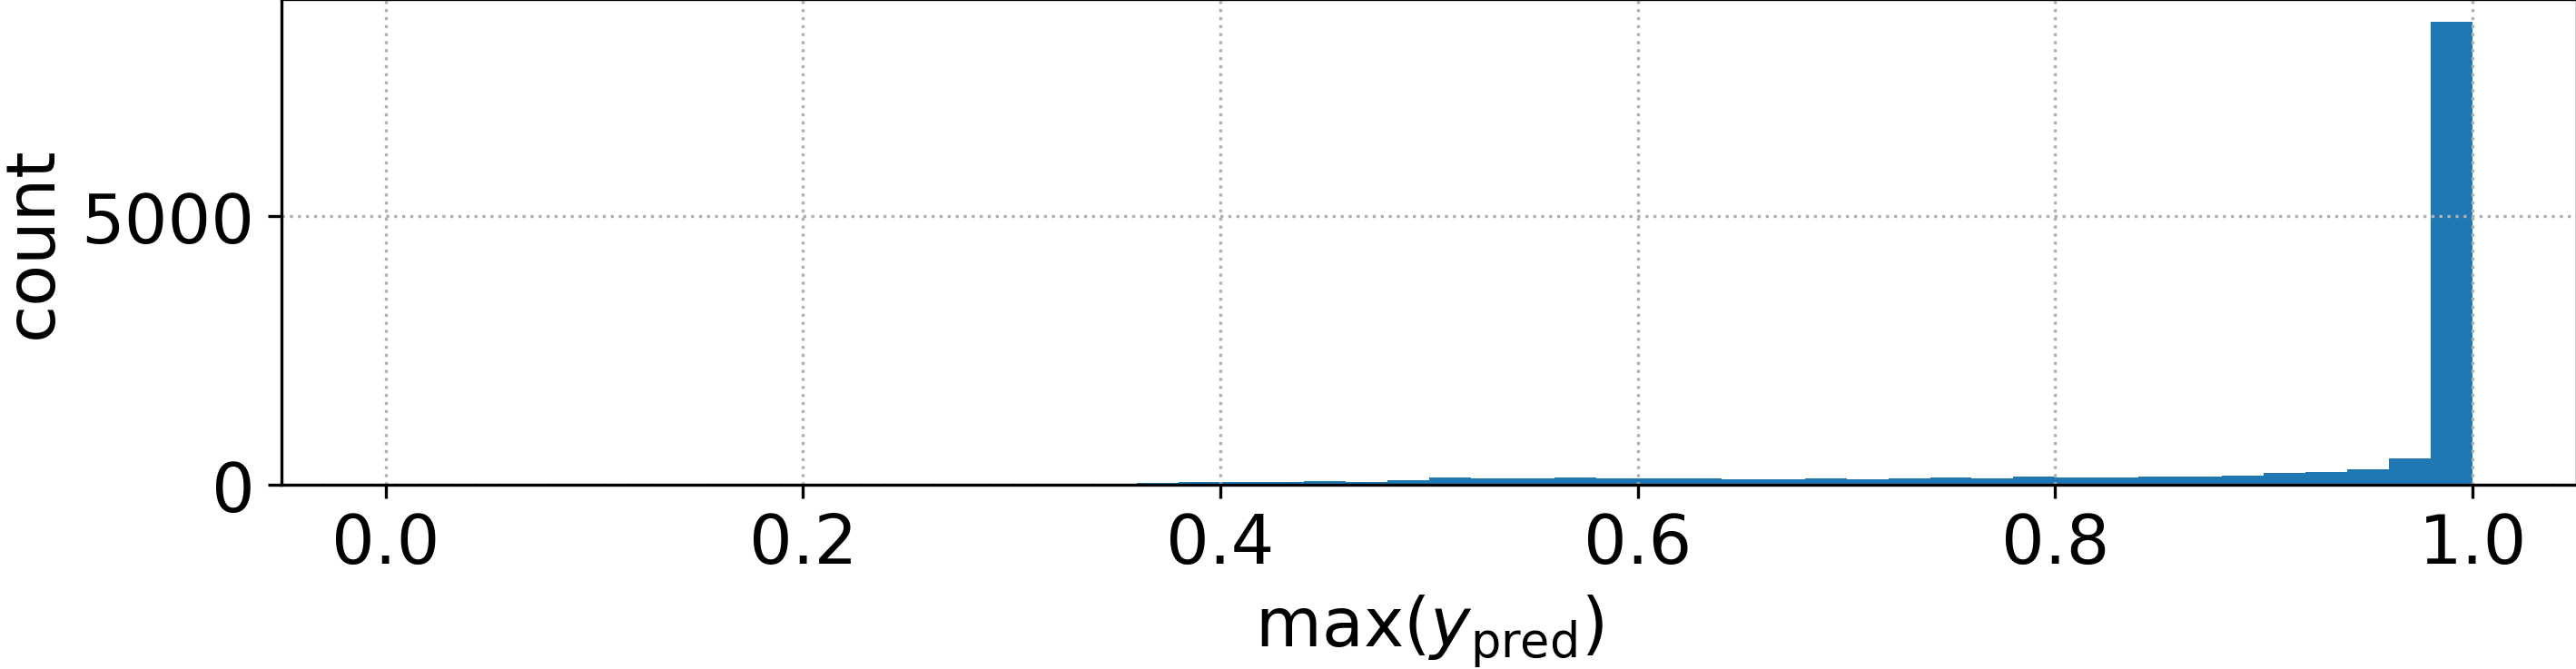
\includegraphics[width=0.8\textwidth]{figures/v1_real/vit_model_V1_original_redomax_ypred_binary_31.png}
        \caption{Spectral ViT V1 Maximum Output Vector Value\label{fig:v1_max}}
    \end{figure}
\end{frame}

\begin{frame}{Spectral ViT V1 Cuts}
    \begin{figure}[b]
        \centering
        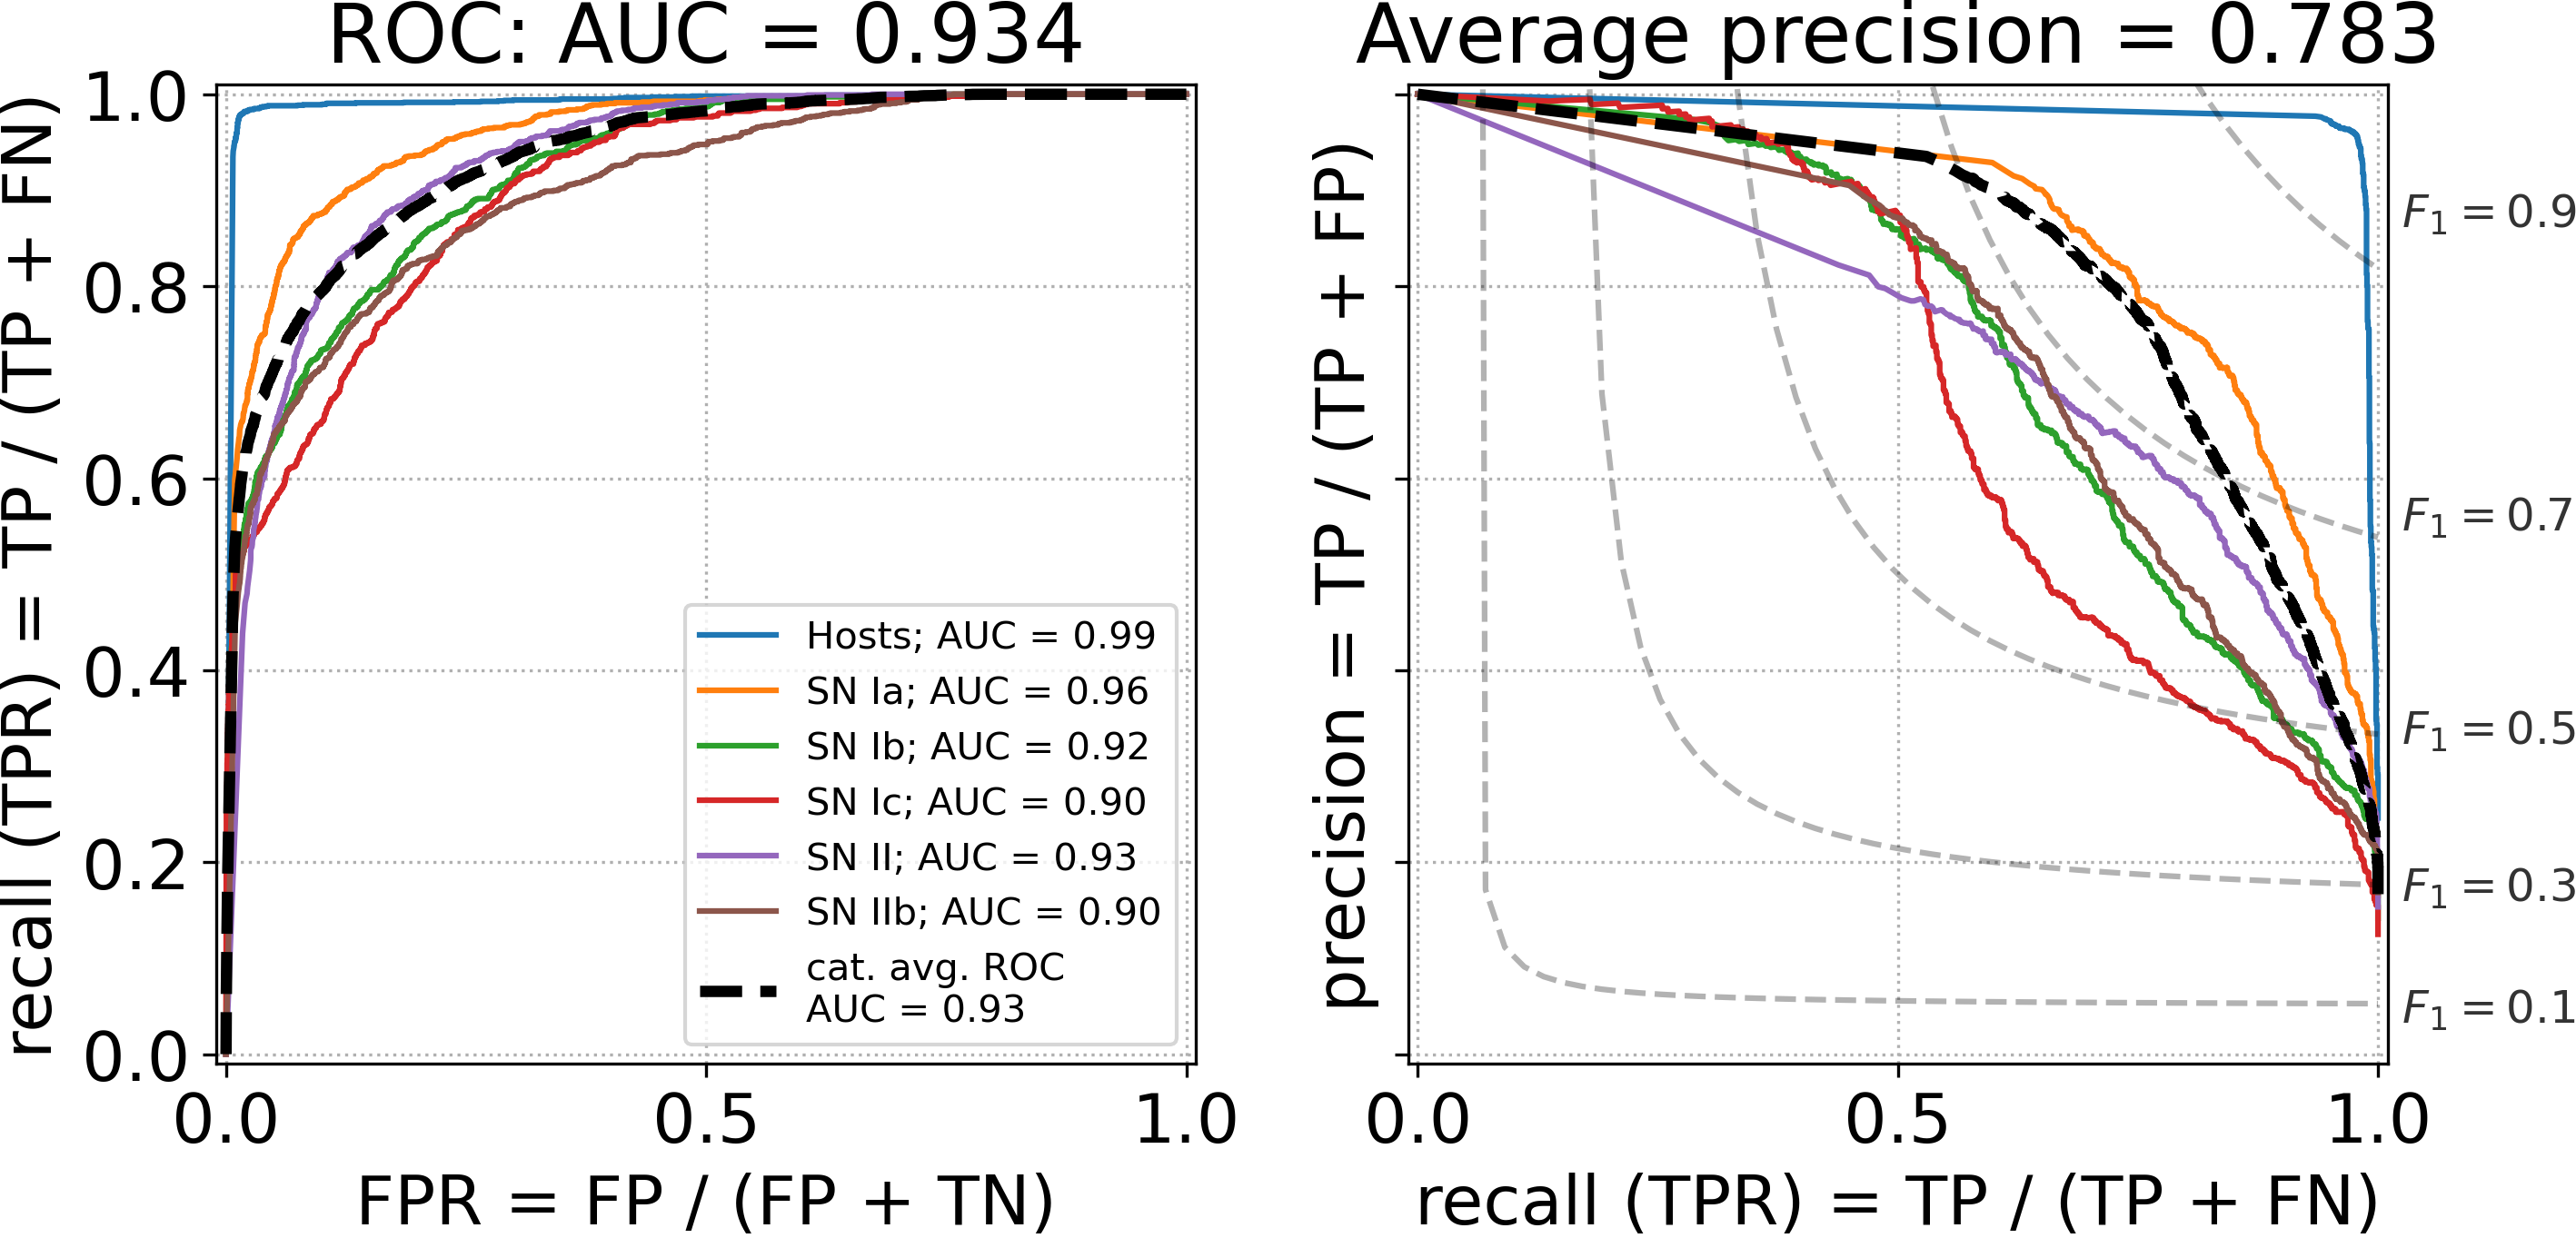
\includegraphics[height=2.6cm]{figures/v1_real/vit_model_V1_original_redoroc99_e31.png}
        \quad
        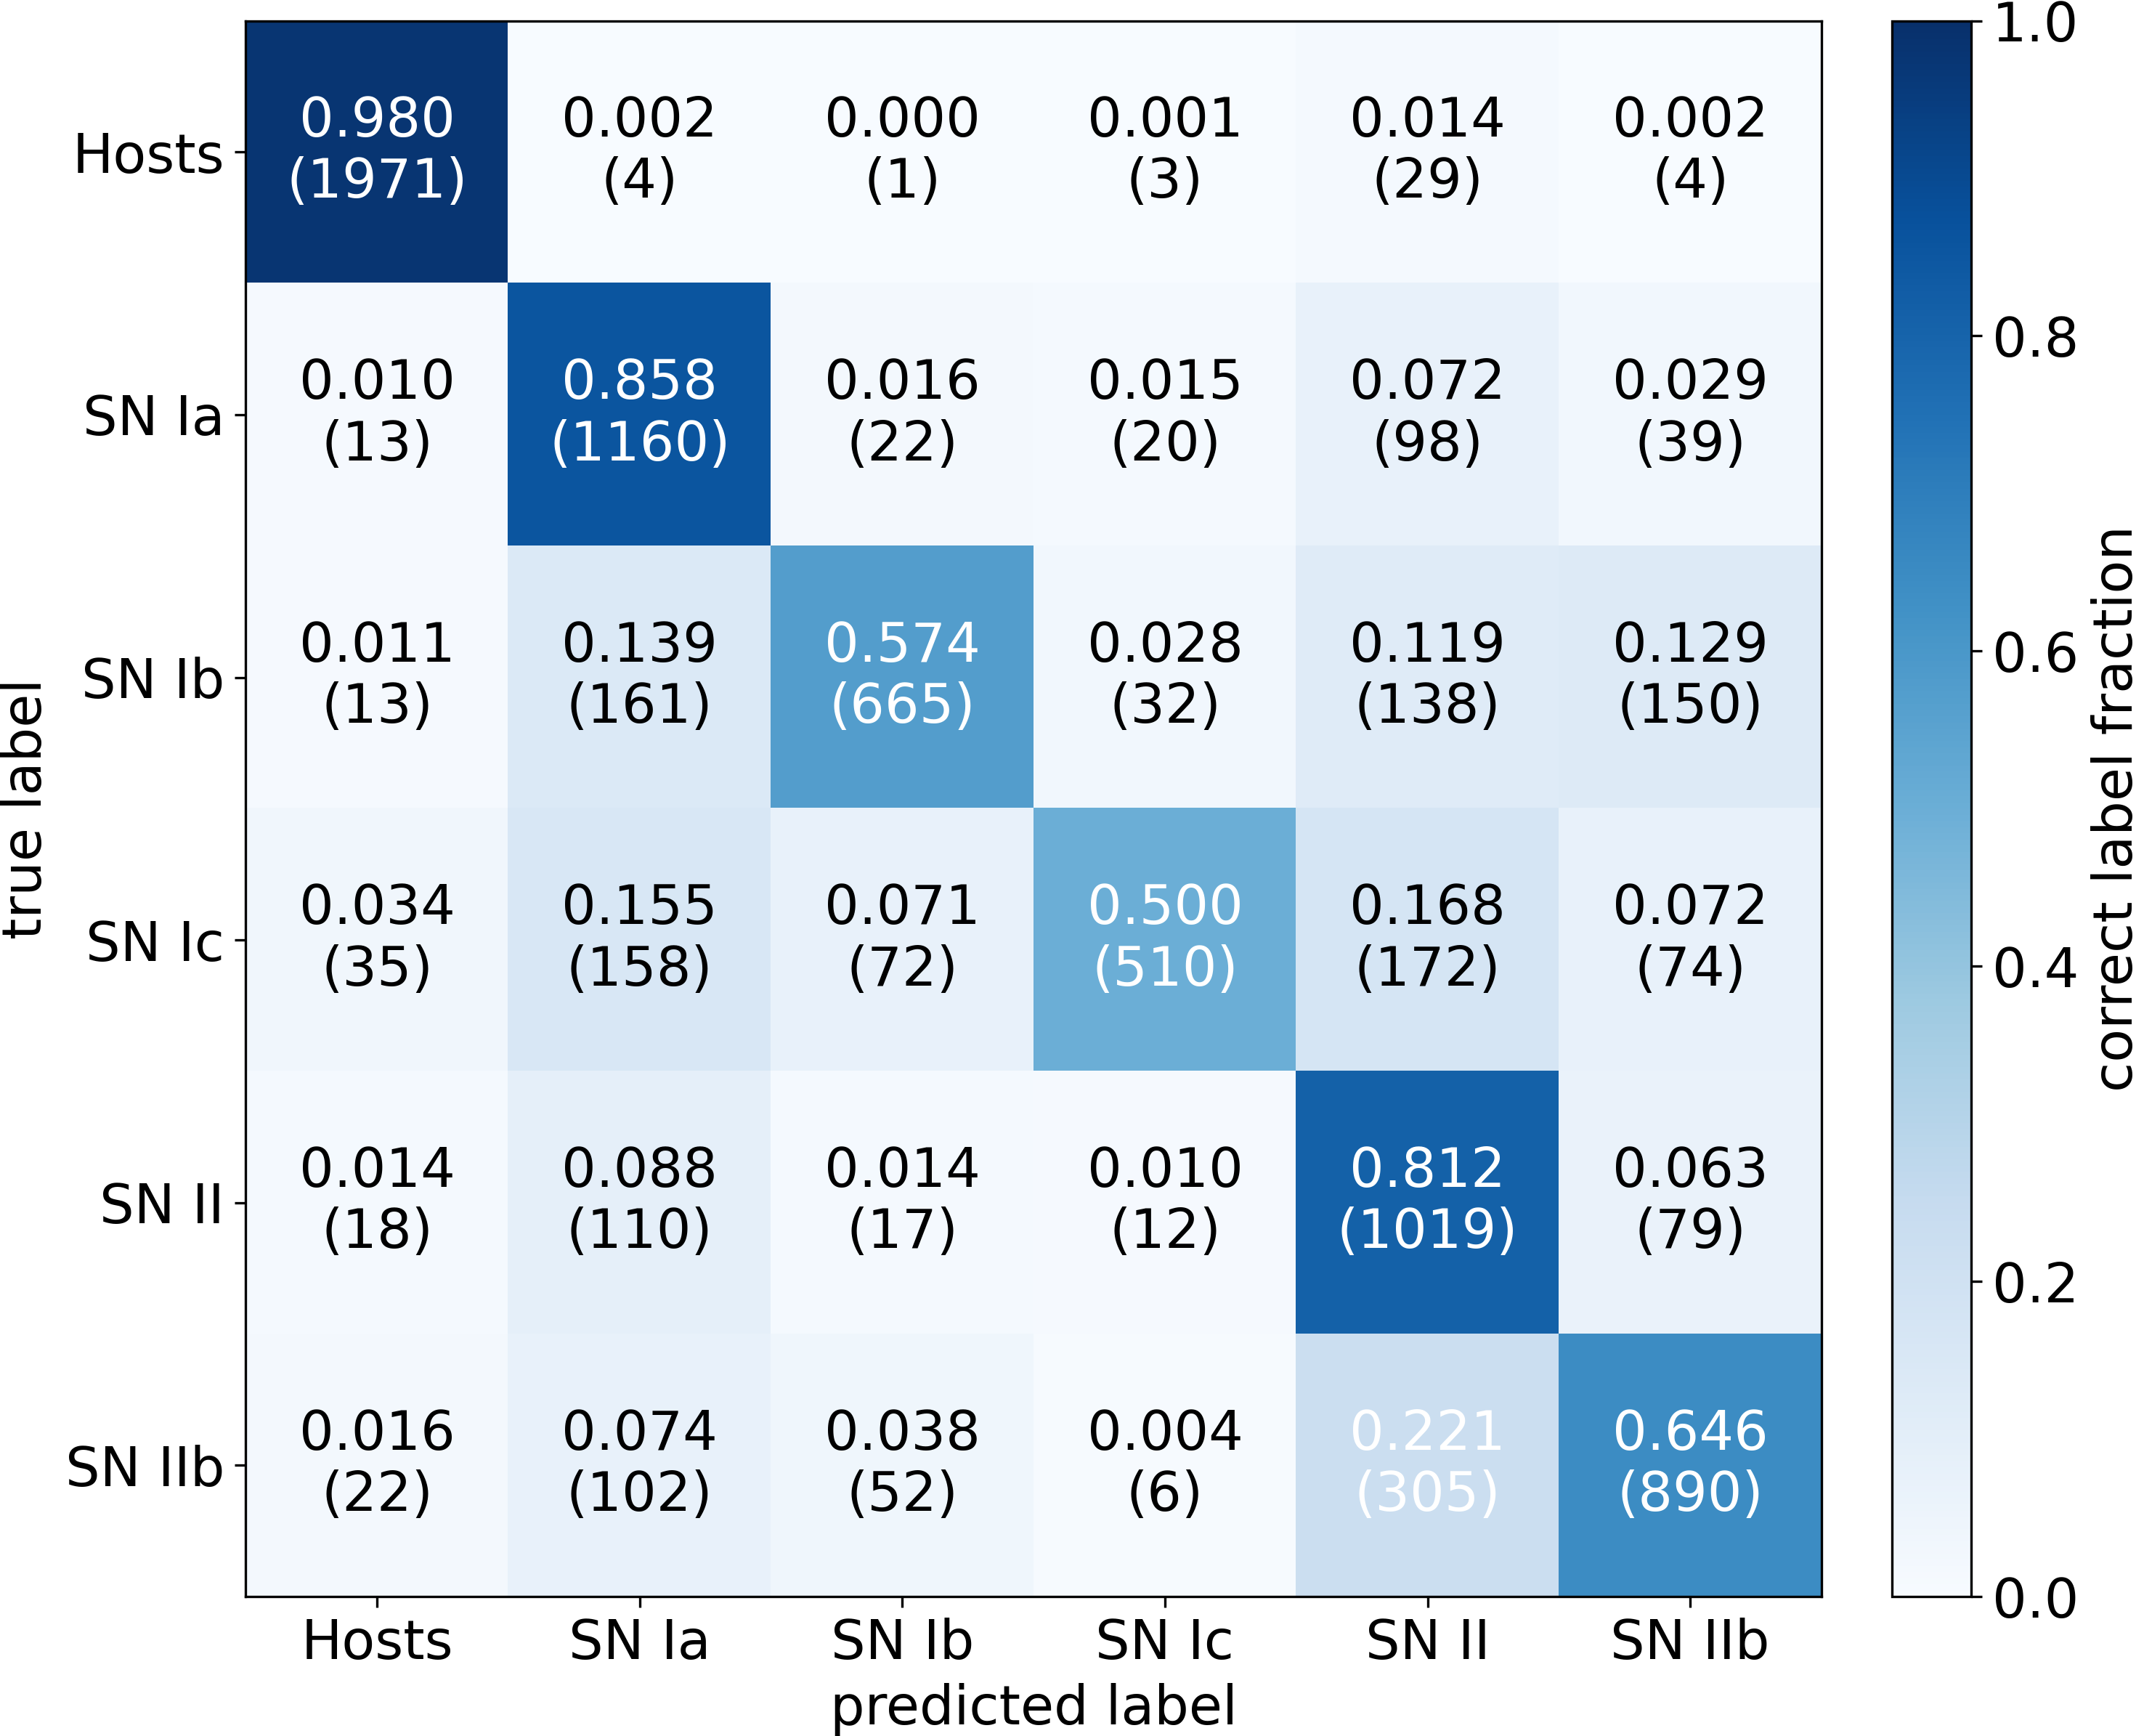
\includegraphics[height=2.6cm]{figures/v1_real/vit_model_V1_original_redocm99_e31.png}
        \caption{Spectral ViT V1 Classifier: 99\% confidence cut \label{fig:v1_99_qual}}
        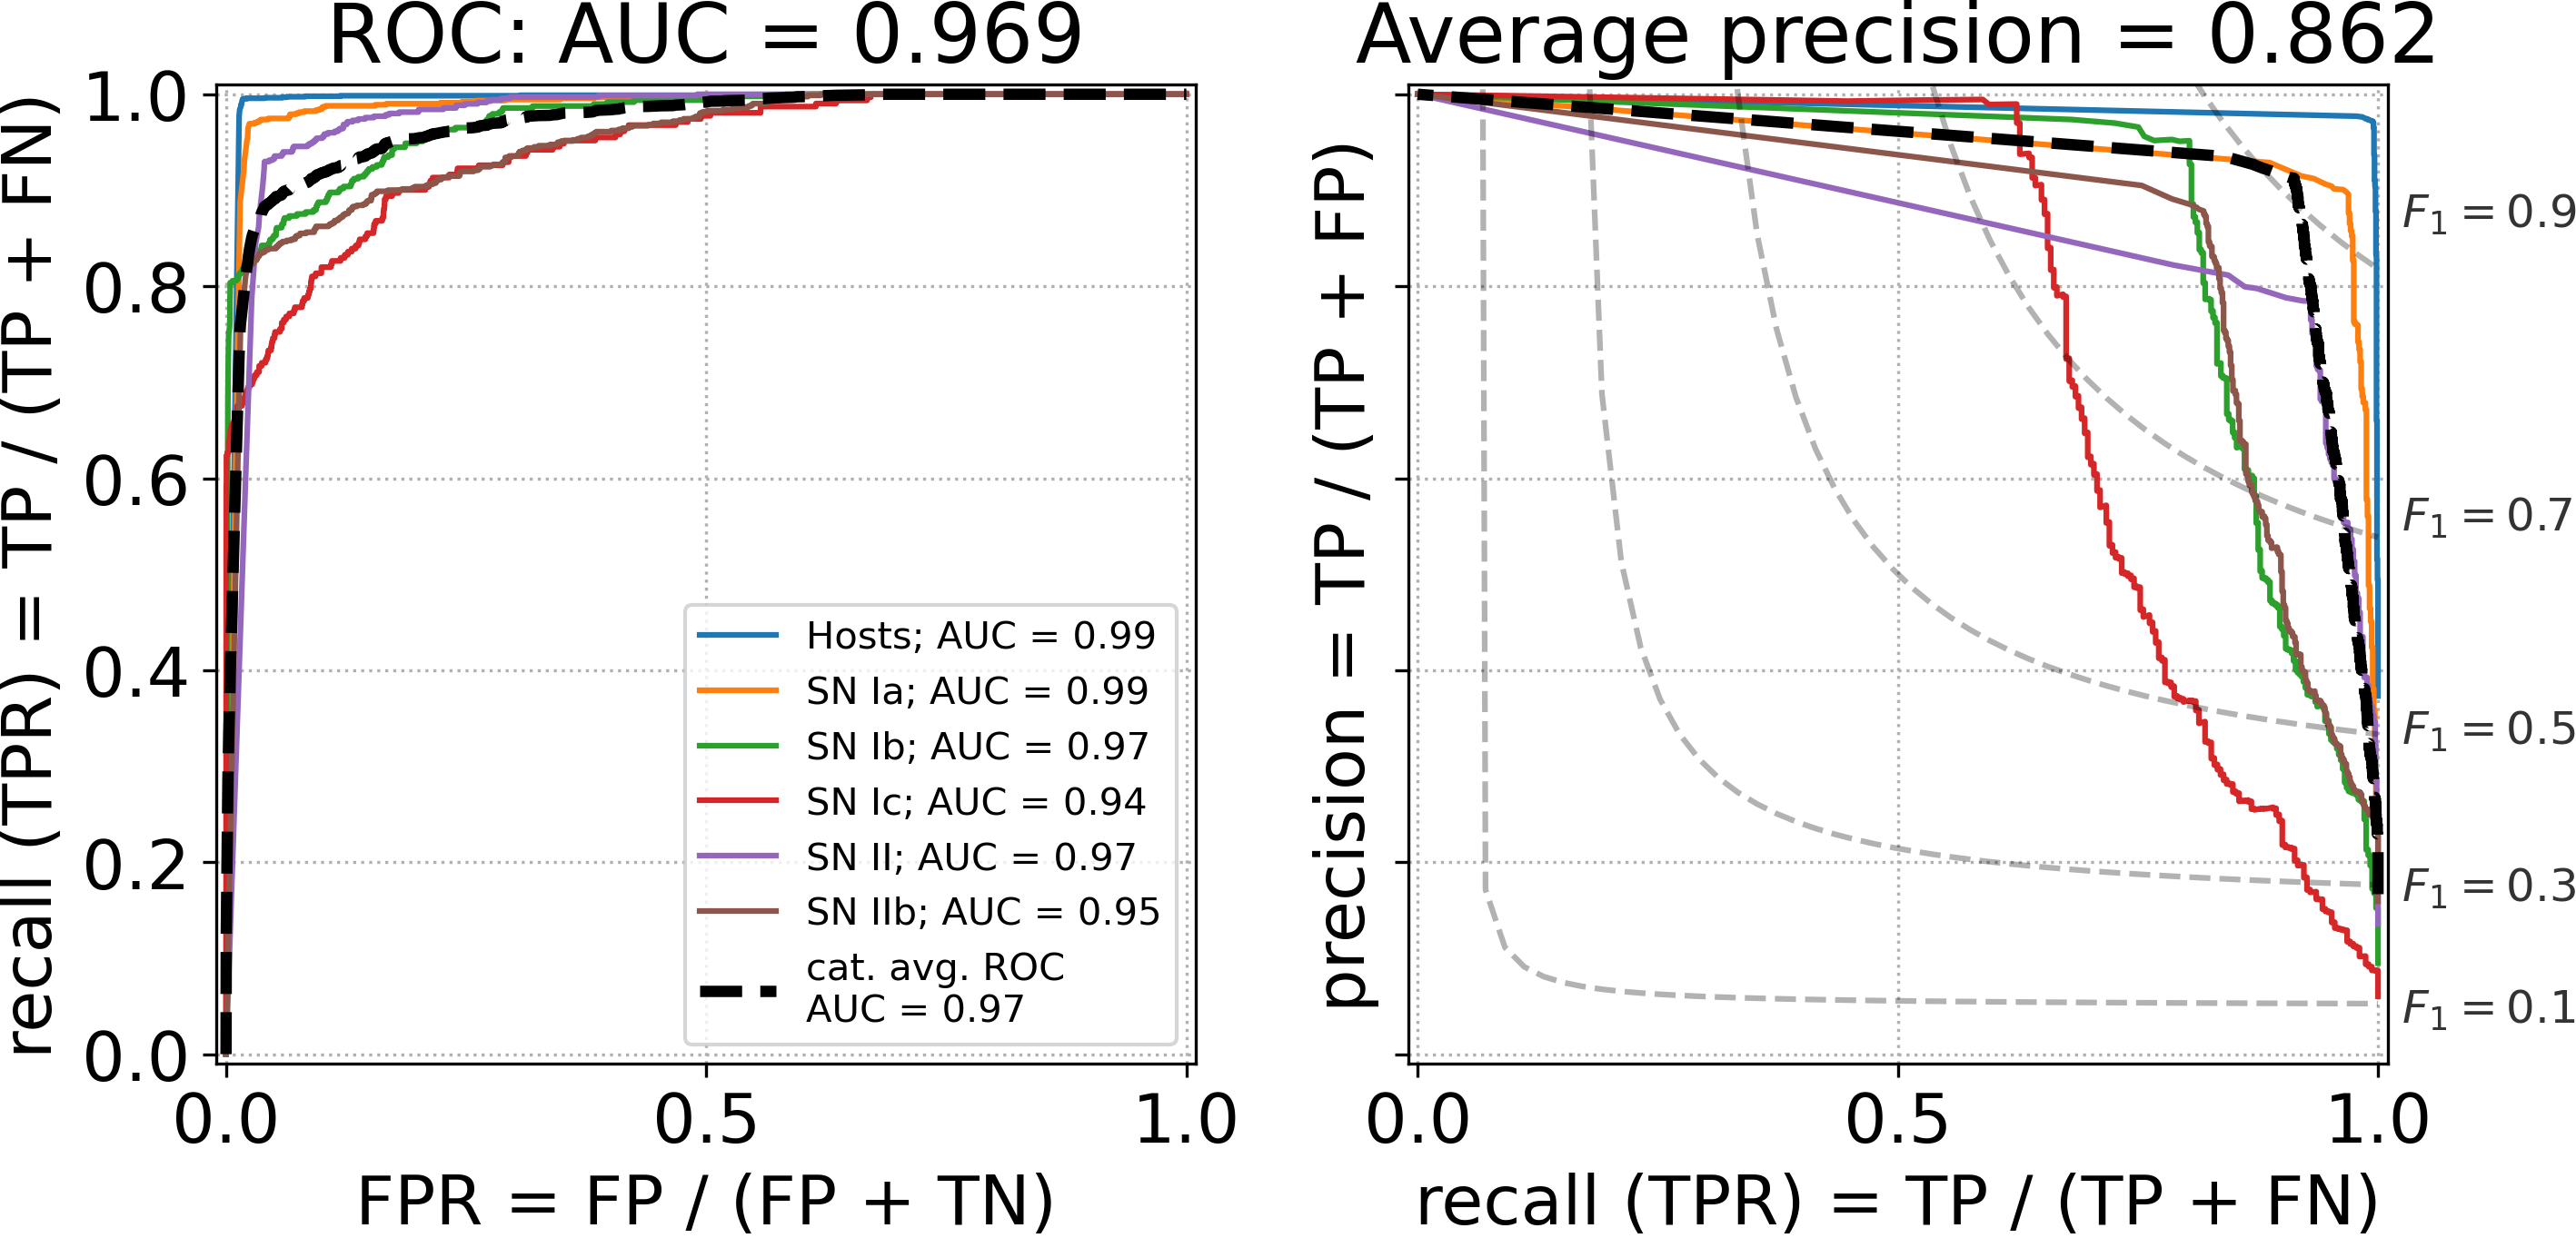
\includegraphics[height=2.6cm]{figures/v1_real/vit_model_V1_original_redoroc999999_e31.png}
        \quad
        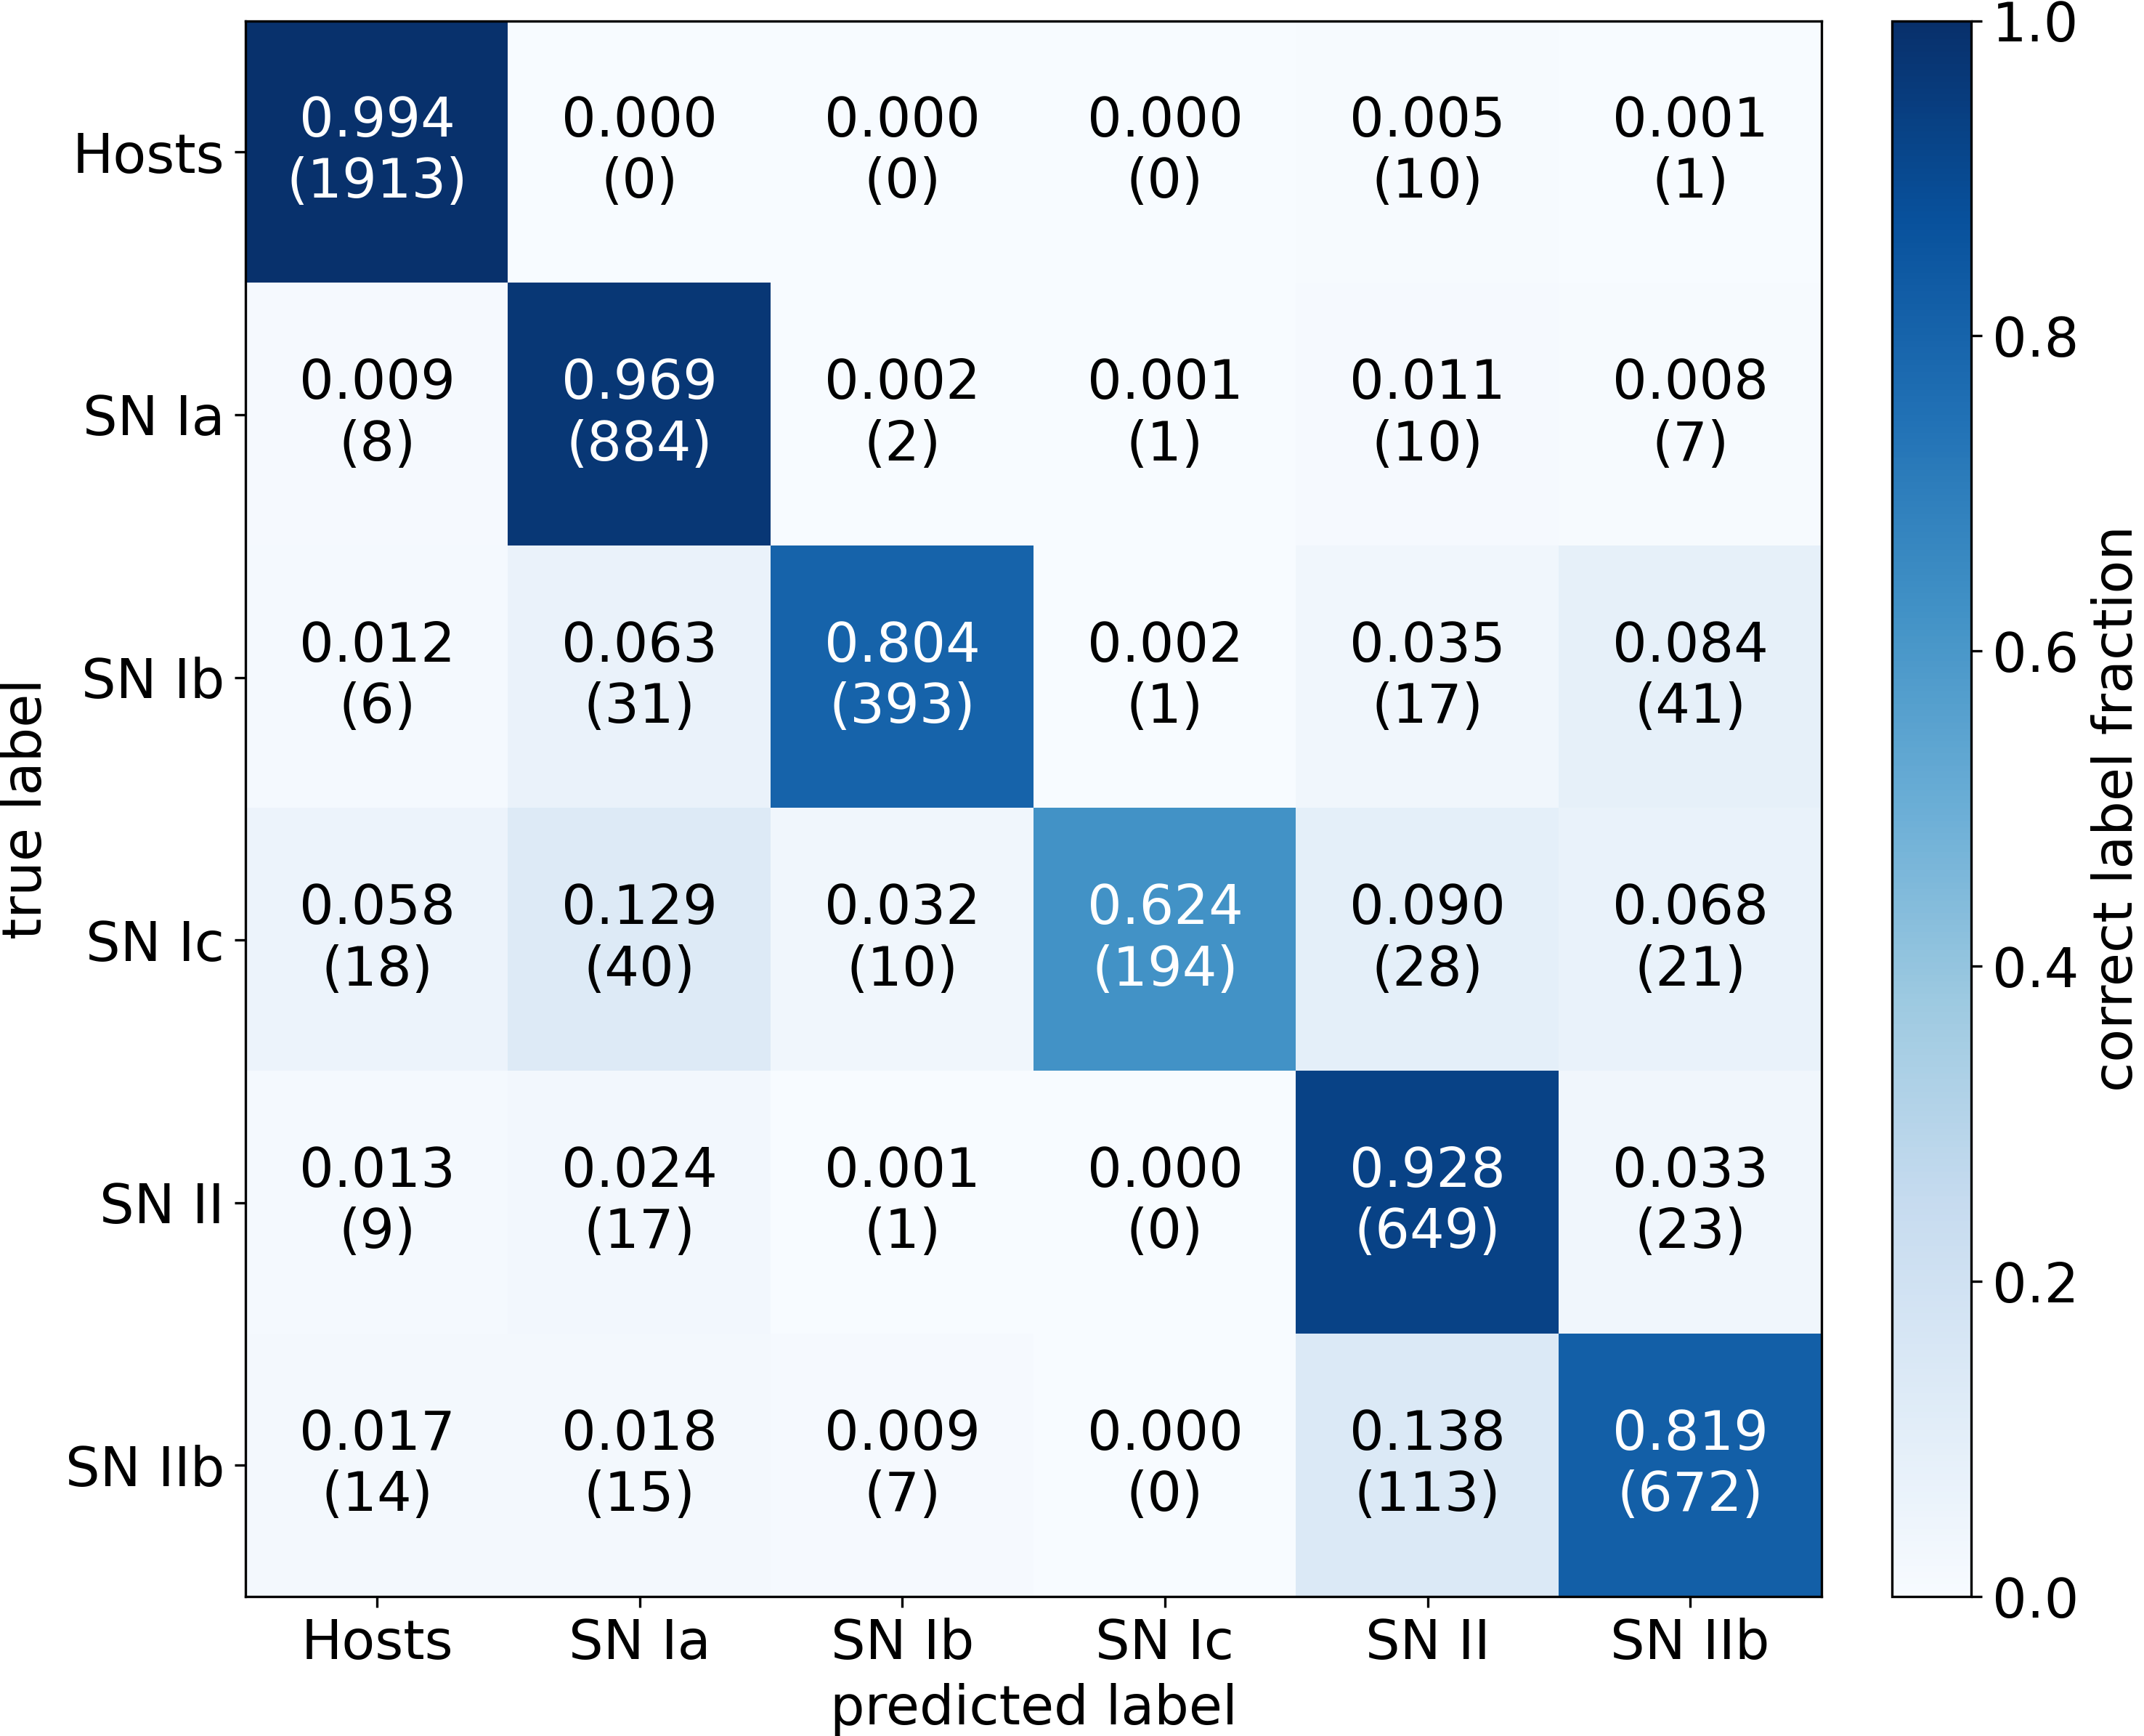
\includegraphics[height=2.6cm]{figures/v1_real/vit_model_V1_original_redocm999999_e31.png}
        \caption{Spectral ViT V1 Classifier: 99.9999\% confidence cut \label{fig:v1_999999_qual}}
    \end{figure}
\end{frame}

% \section{Spectral ViT V2: Specialized Classifier}
\begin{frame}
    \begin{figure}[b!]
        \centering
        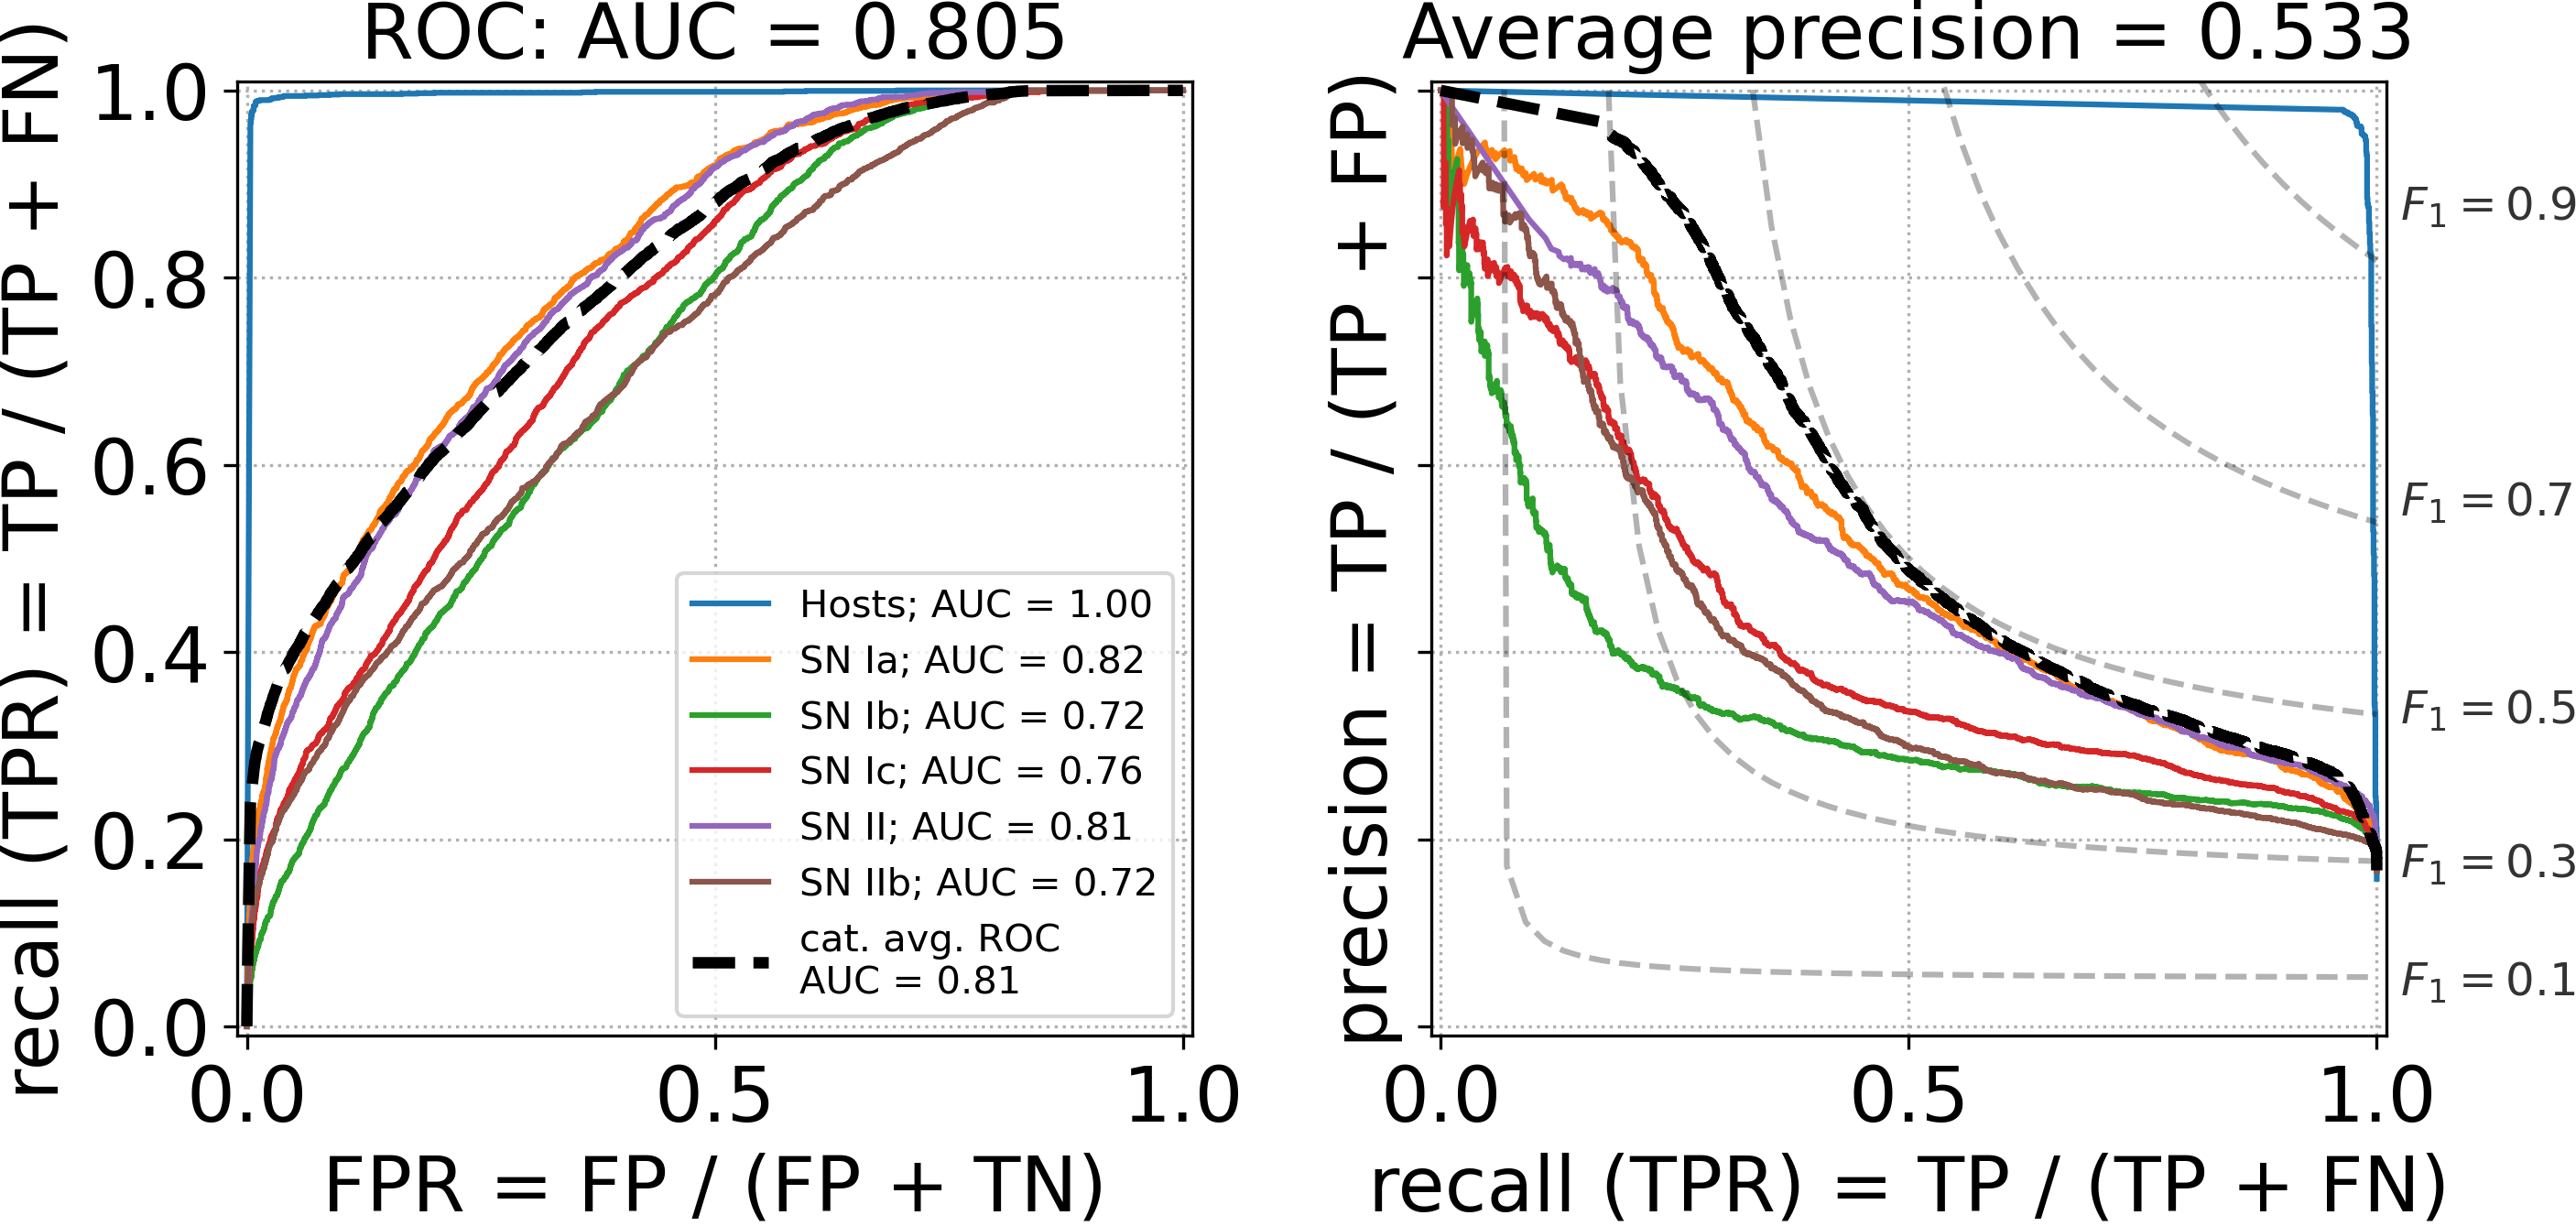
\includegraphics[height=2.8cm]{figures/v2_real/vit_model_V2rocfulle_e26.png}
        \quad
        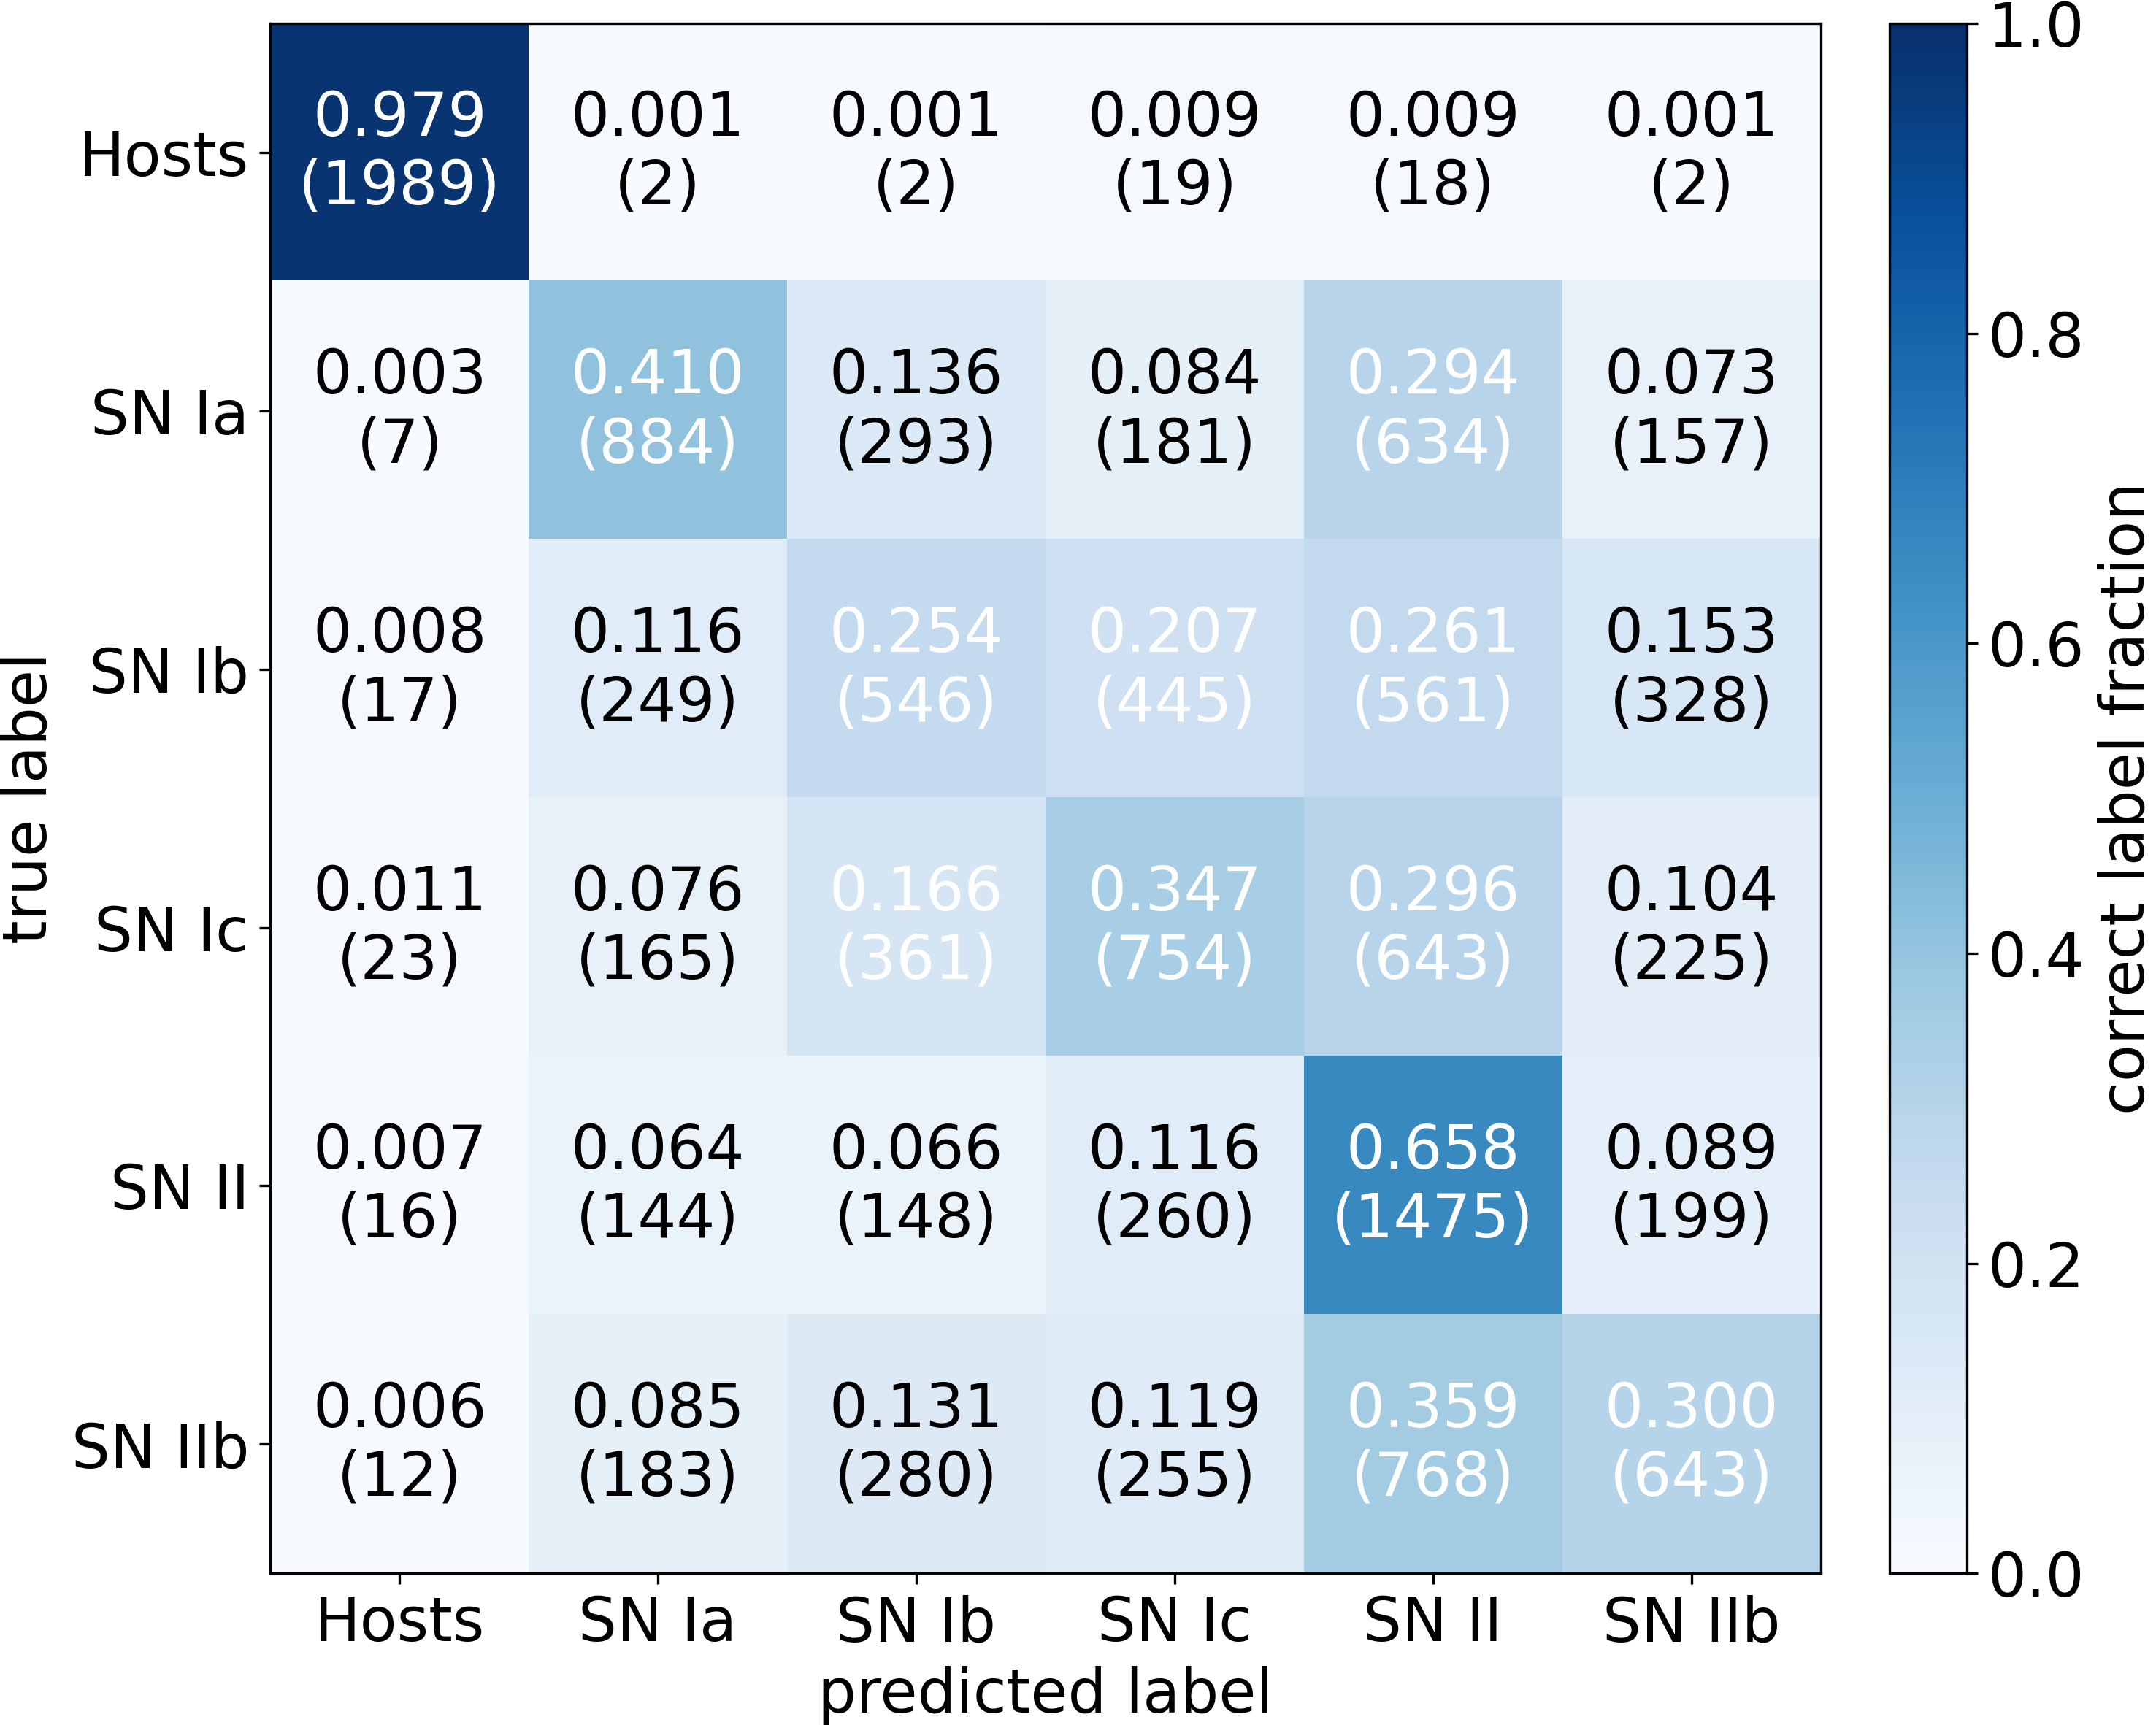
\includegraphics[height=2.8cm]{figures/v2_real/vit_model_V2cmfull_e26.png}
        \caption{Spectral ViT V2 Classifier\label{fig:v2_qual}}
%     \end{figure}
% \end{frame}

% \begin{frame}
%     \begin{figure}[t!]
%         \centering
        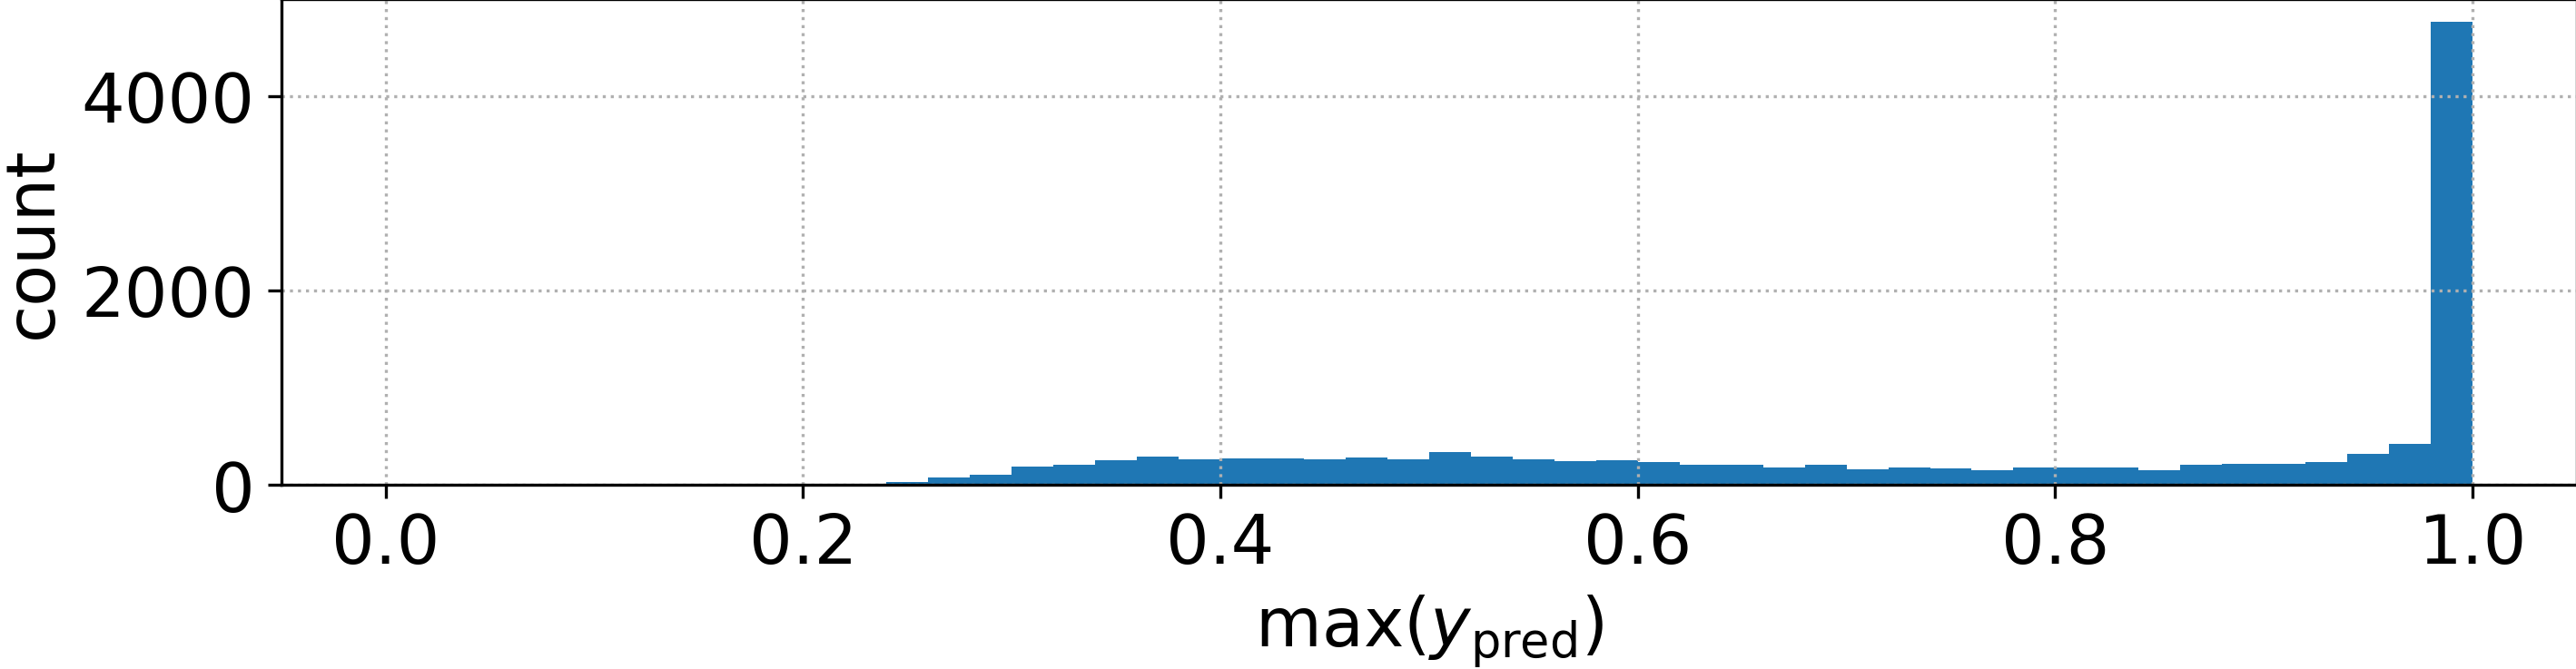
\includegraphics[width=0.8\textwidth]{figures/v2_real/vit_model_V2max_ypred_26.png}
        \caption{Spectral ViT V2 Maximum Output Vector Value\label{fig:v2_max}}
    \end{figure}
\end{frame}

\begin{frame}
    \begin{figure}[b!]
        \centering
        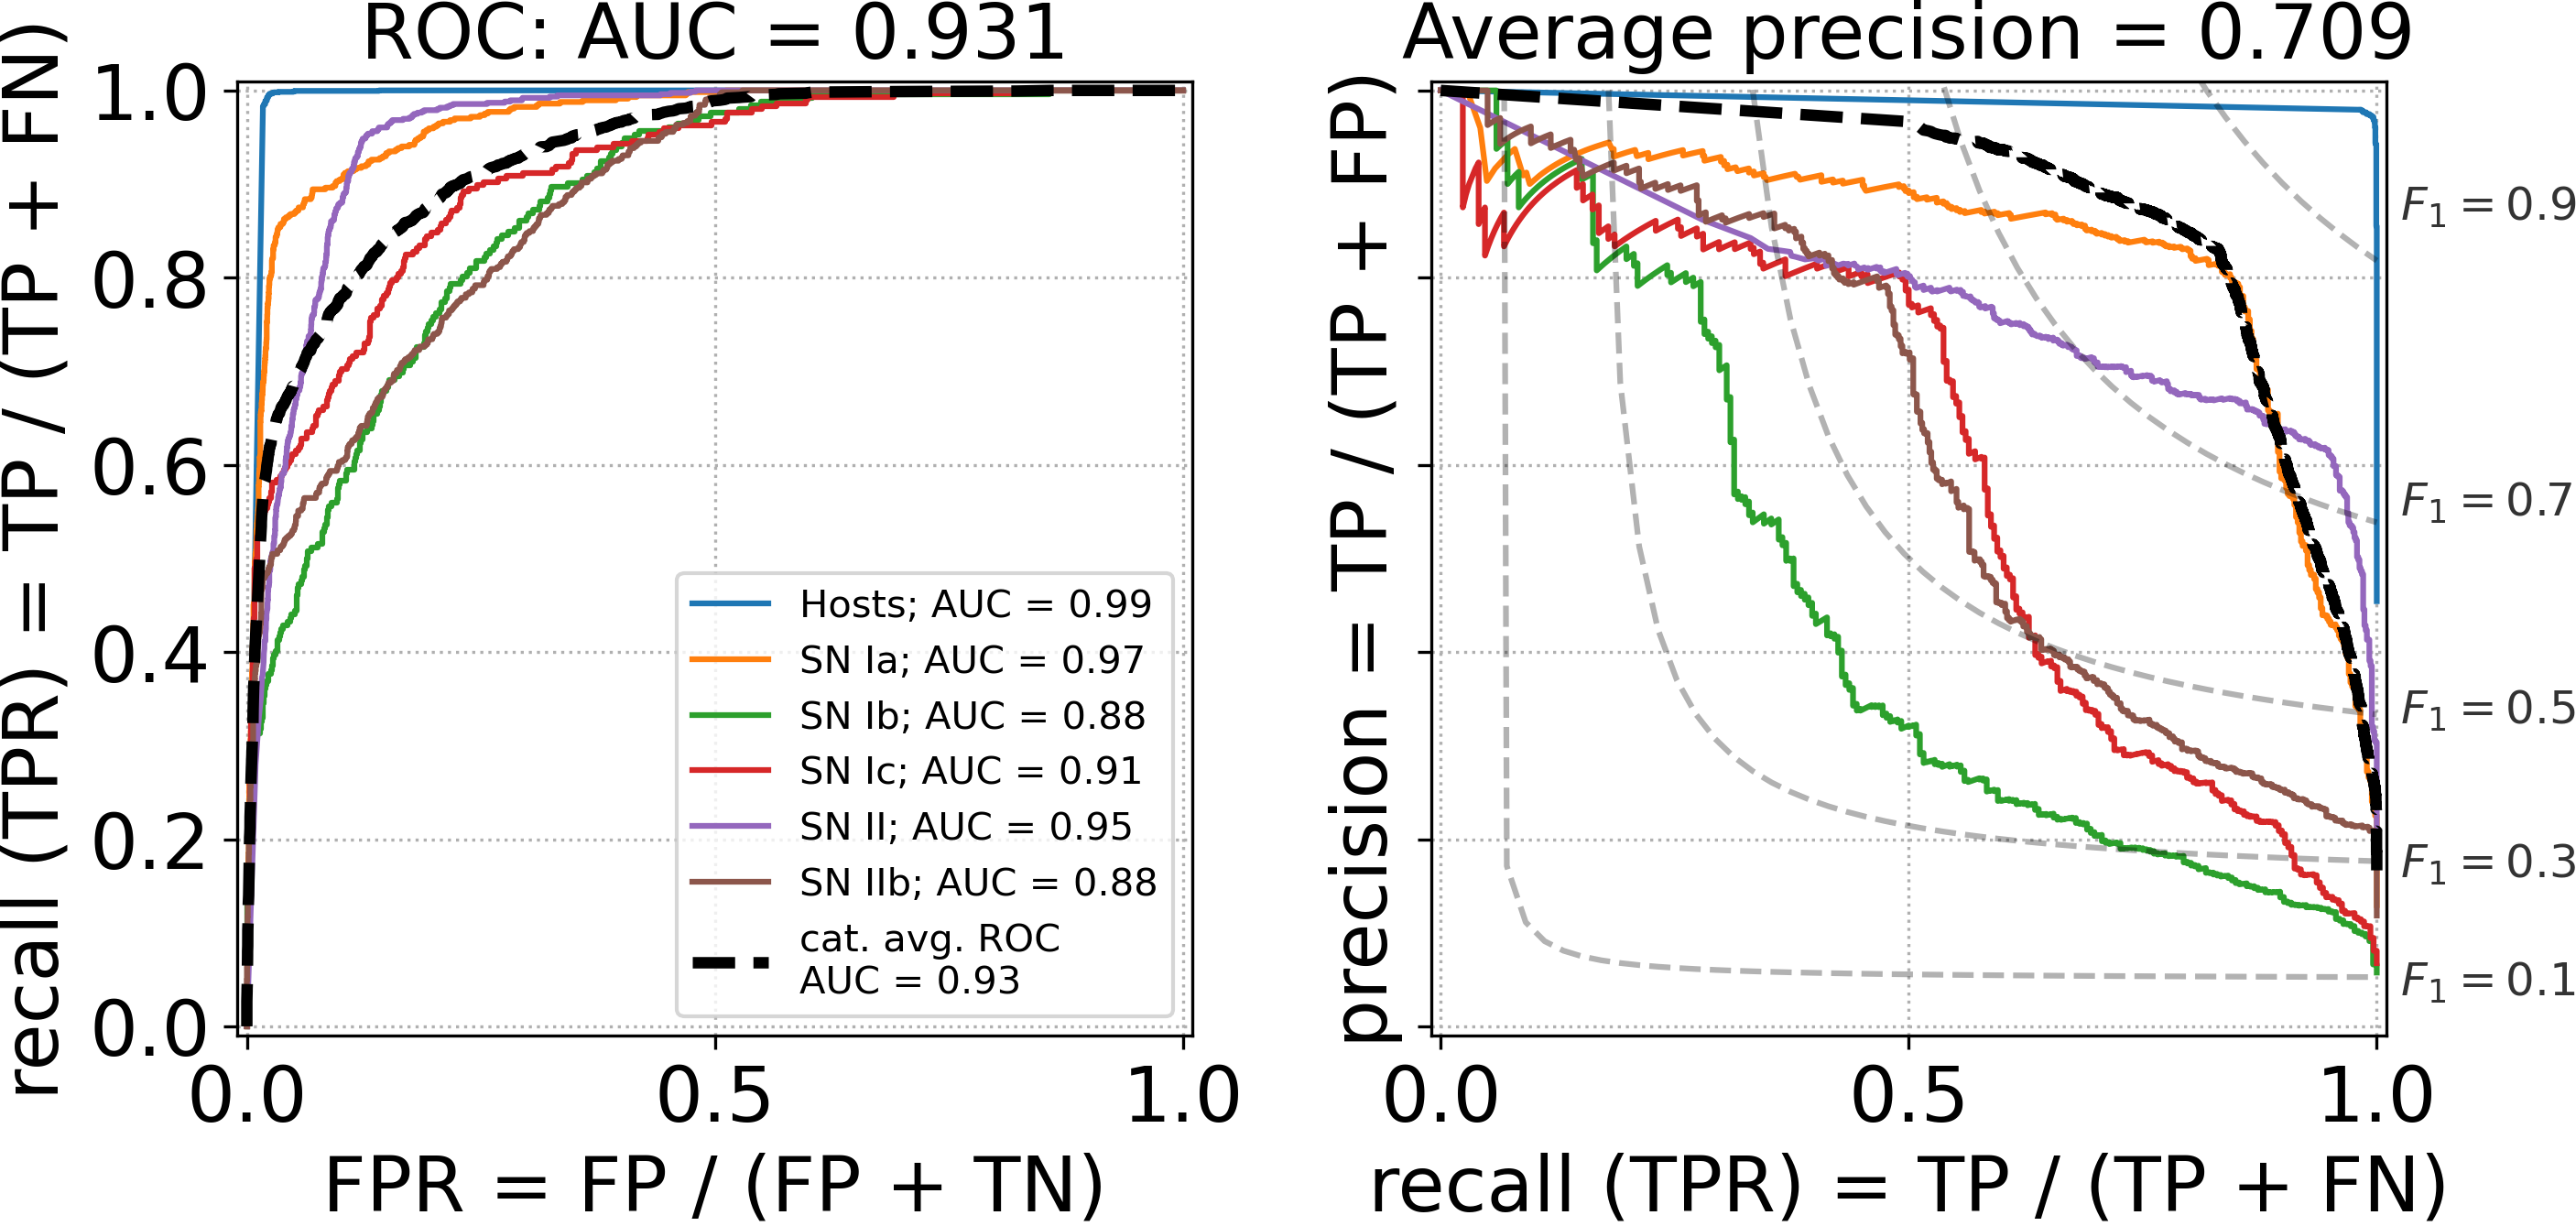
\includegraphics[height=2.8cm]{figures/v2_real/vit_model_V2roc99_e26.png}
        \quad
        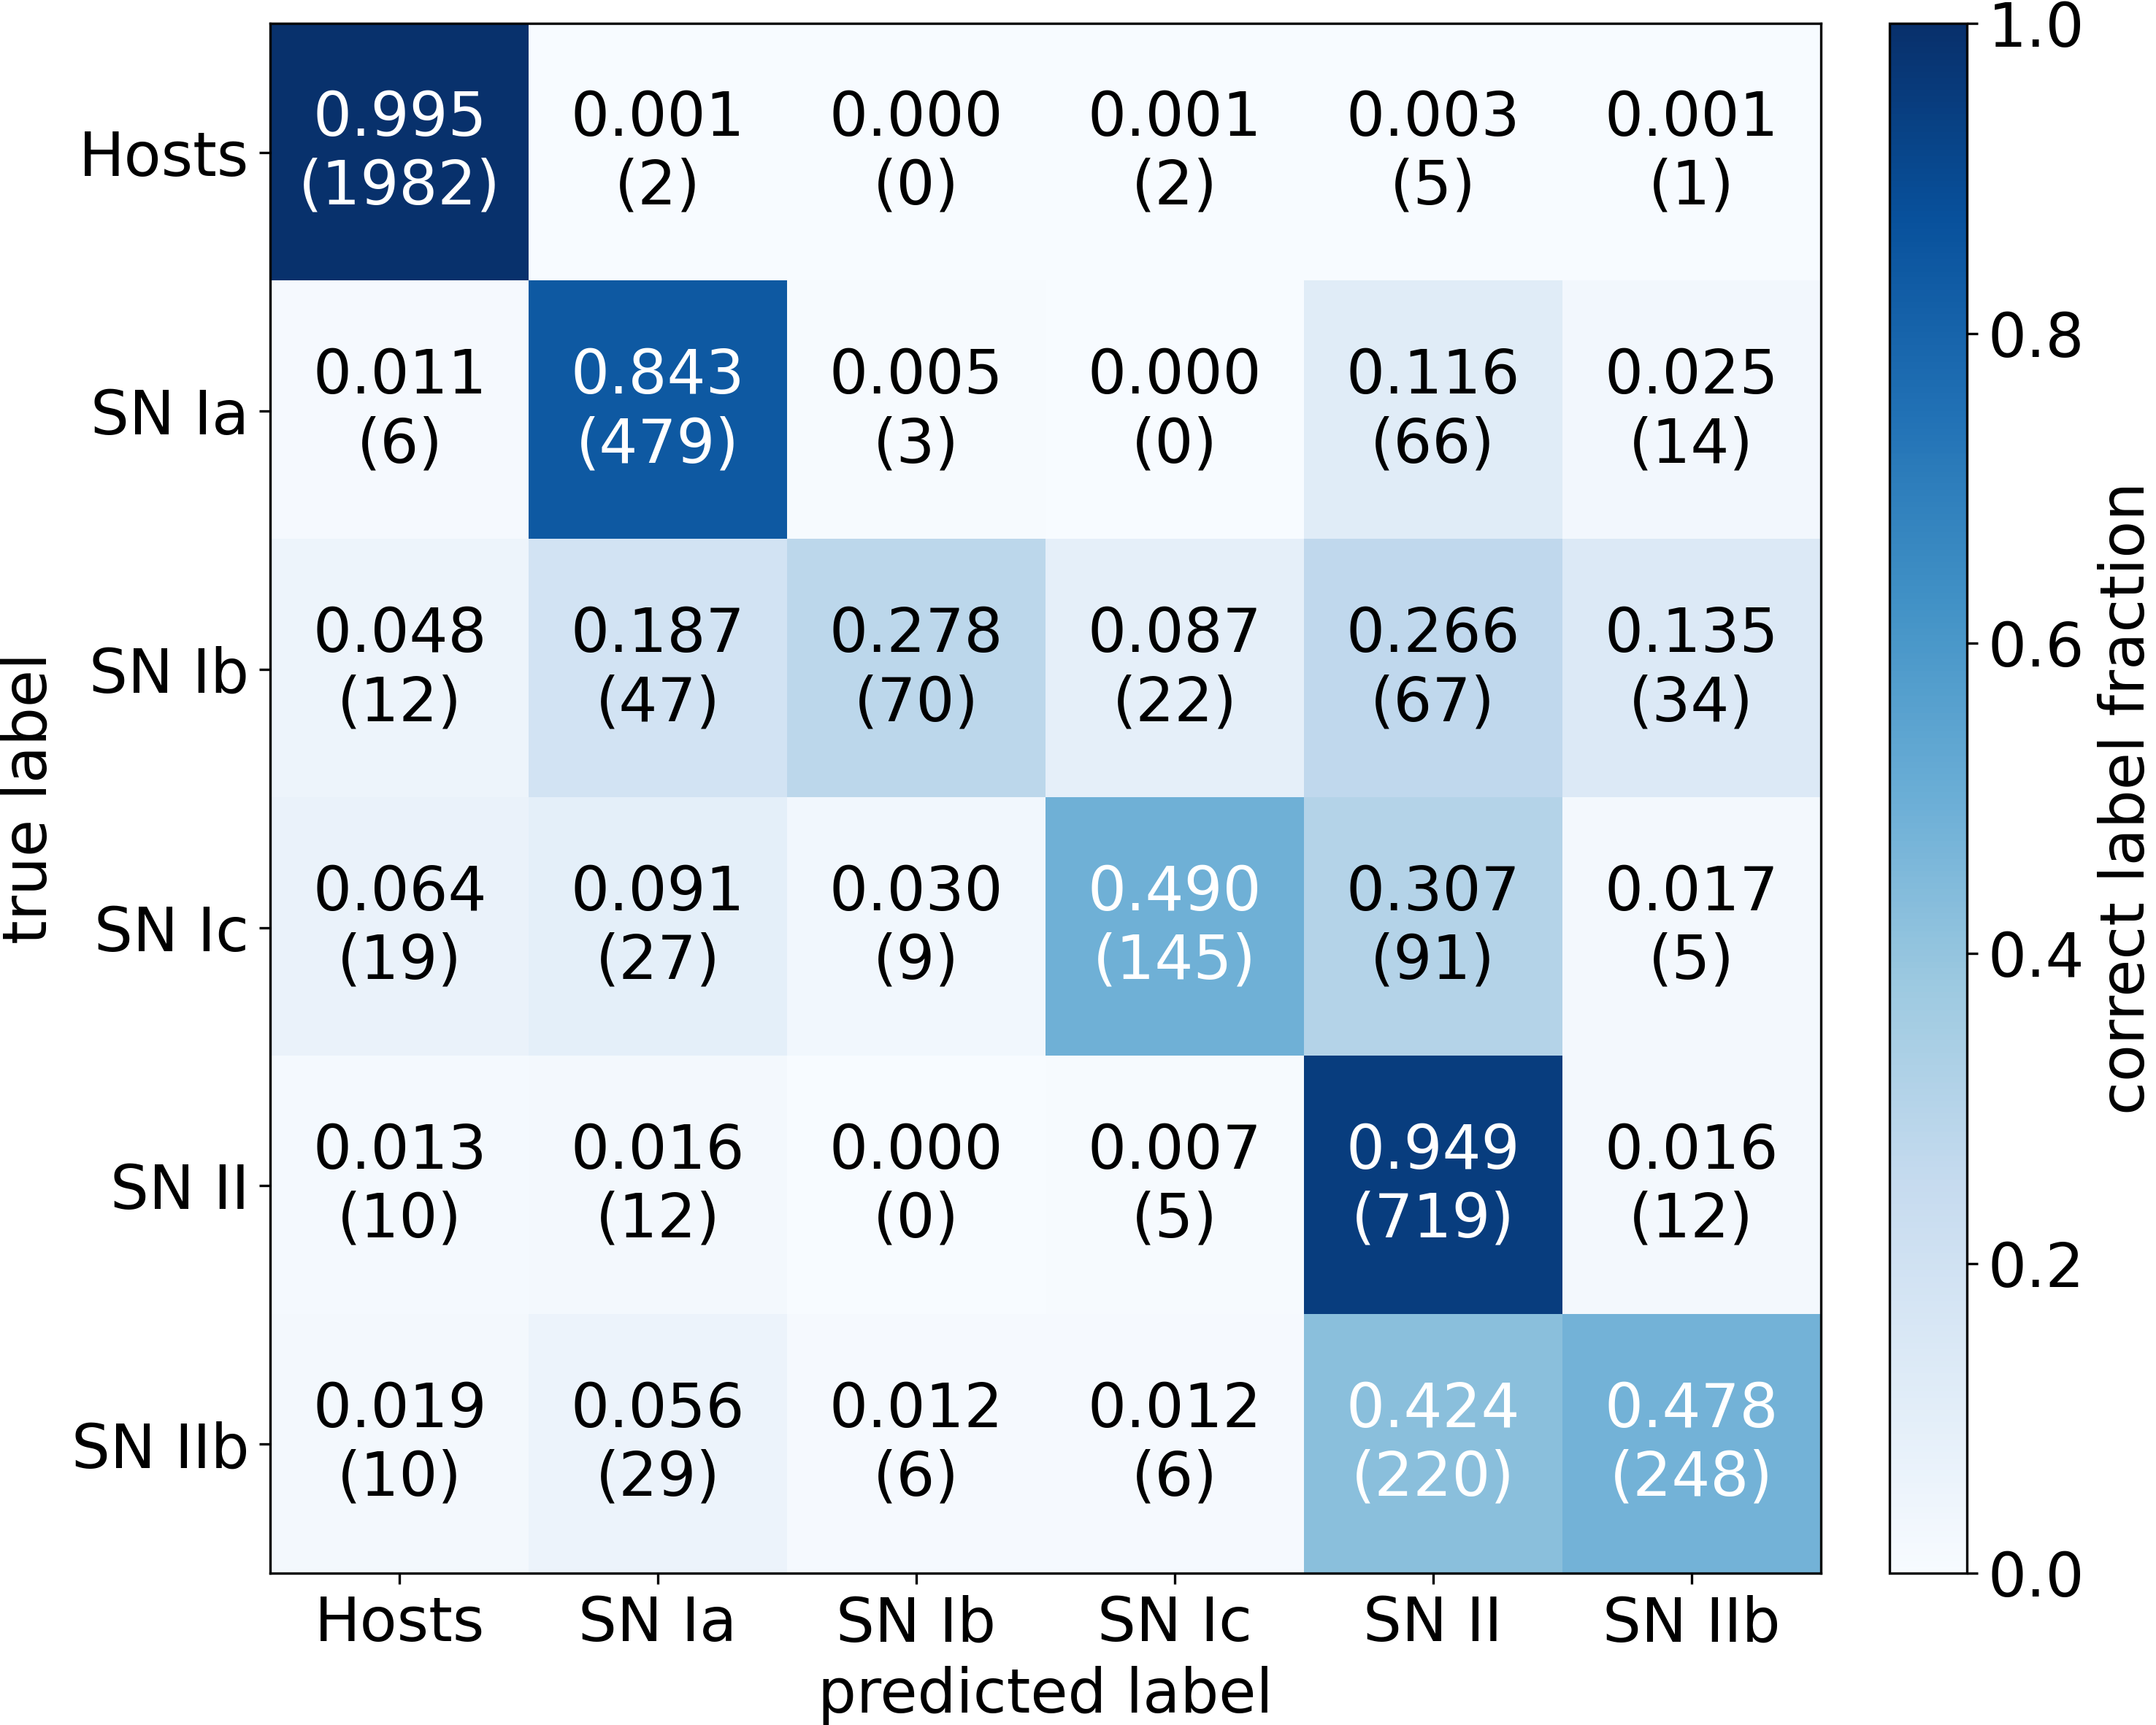
\includegraphics[height=2.8cm]{figures/v2_real/vit_model_V2cm99_e26.png}
        \caption{Spectral ViT V2 Classifier (99\% confidence cut)\label{fig:v2_99_qual}}
    \end{figure}
\end{frame}


\begin{frame}{Binary Classifier}
    \begin{figure}[t!]
        \centering
        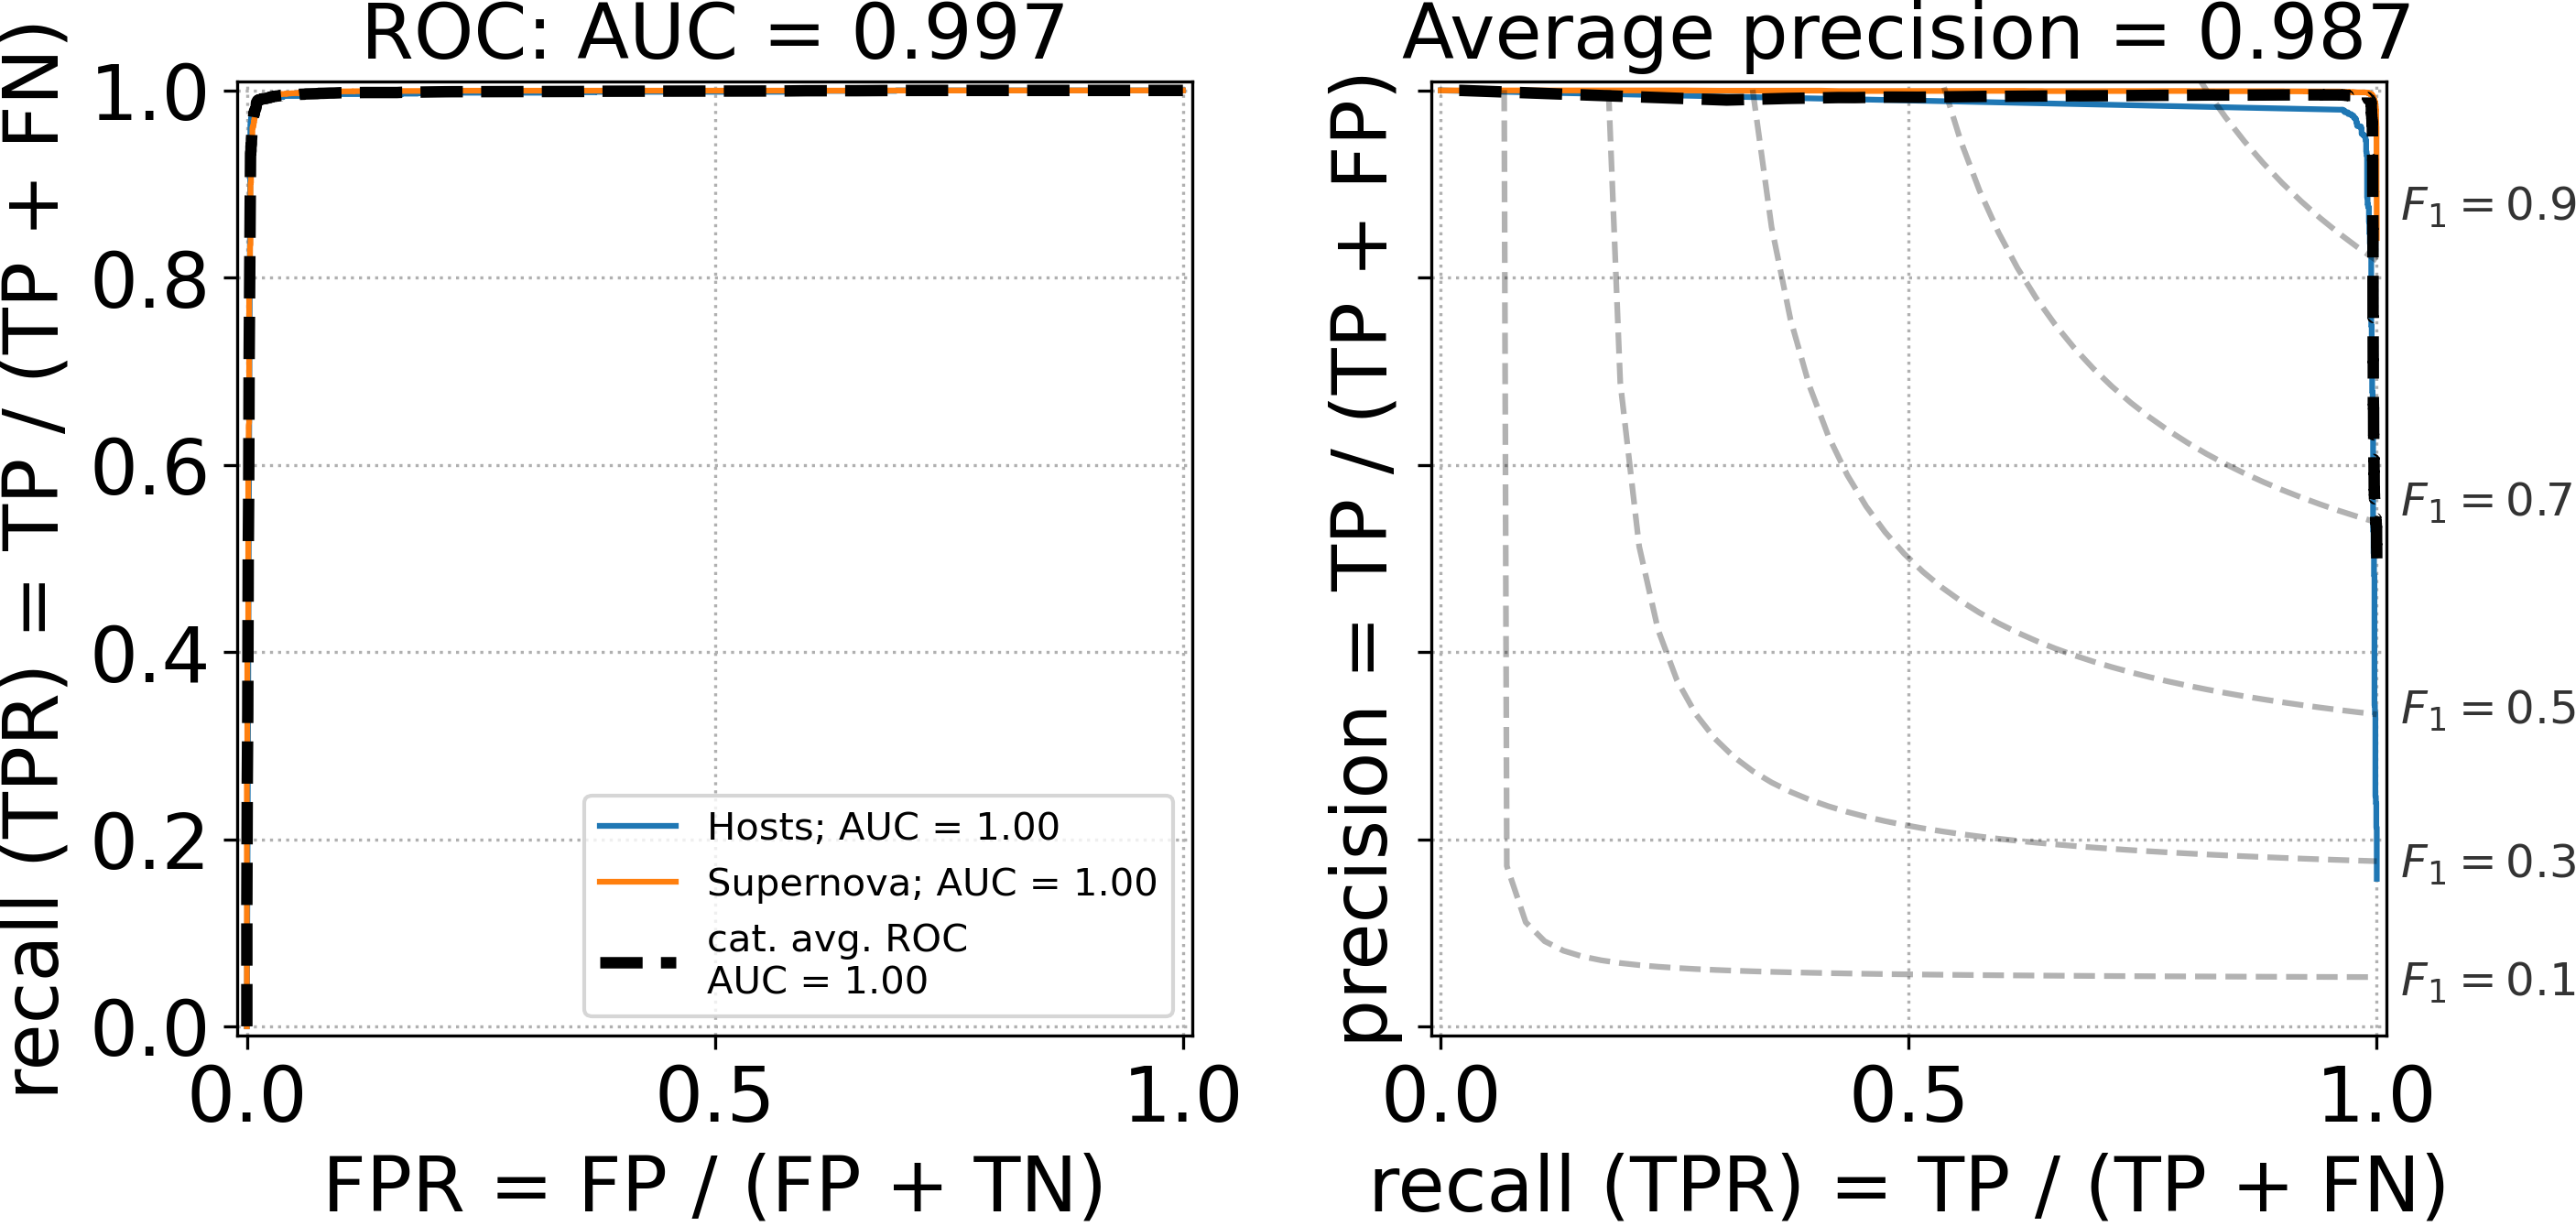
\includegraphics[height=2.7cm]{figures/v2_real/vit_model_V2rocfull_binary_e26.png}
        \quad
        \includegraphics[height=2.7cm]{figures/v2_real/vit_model_V2cmfull_binary_e26.png}
        \caption{Spectral ViT V2 Binary Classifier\label{fig:v2_binary_qual}}
    \end{figure}
\end{frame}

\begin{frame}{Other Classifiers}
    \begin{figure}
        \centering
        \includegraphics[height=2.5cm]{figures/v2_applications/vit_model_V2roc99_proj_e26.png}
        \quad
        \includegraphics[height=2.5cm]{figures/v2_applications/vit_model_V2cm99_proj_e26.png}
        \caption{Spectral ViT V2 Progenitor Classifier (99\% confidence cut)\label{fig:v2_99_proj_qual}}
    % \end{figure}
    % \begin{figure}[t!]
    %     \centering
        \includegraphics[height=2.5cm]{figures/v2_applications/vit_model_V2roc99_type_e26.png}
        \quad
        \includegraphics[height=2.5cm]{figures/v2_applications/vit_model_V2cm99_type_e26.png}
        \caption{Spectral ViT V2 Type Classifier (99\% confidence cut)\label{fig:v2_99_type_qual}}
    \end{figure}
\end{frame}



% \begin{figure}[h]
%     \centering
%     \includegraphics[height=2.7cm]{figures/v2_real/vit_model_V2roc9999_binary_e26.png}
%     \quad
%     \includegraphics[height=2.7cm]{figures/v2_real/vit_model_V2cm9999_binary_e26.png}
%     \caption{Spectral ViT V2 Binary Diagnostics: ROC Curve (left) and Confusion Matrix (right) with a 99.99\% confidence
%     cut \label{fig:v2_binary_9999_qual}}
% \end{figure}


\begin{comment}
\begin{frame}
    \frametitle{Results}
    \small
    \begin{table}[]
        \centering
        \caption{Best performance after 25 epochs of training.}
        \resizebox{\linewidth}{!}{\begin{tabular}{lccc}
	\toprule
    \textbf{Spam} & \textbf{Ni} & \textbf{Swallow} & \textbf{Shrubbery} \\
    \midrule
    A & 1 & 2 & 3 \\
    \midrule
    E & 3 & 4 & 5 \\
    C & 6 & 9 & 3 \\
    \midrule
    M & 4 & 1 & 1 \\
    \bottomrule
\end{tabular}}
    \end{table}
\end{frame}
%%%%%%%%%%%%%%%%%%%%%%%%%%%%%%%%%%%%%%%%%%%%%%%%%%%%%%%%%%%%%%%%%%%%%%%%
\begin{frame}
    \frametitle{Results -- Classification}
    \begin{figure}[t]
        \centering
        \includegraphics[width=0.8\linewidth]{figures/blackbox.jpeg}
        \caption{Predictions after training on the full HAM10000 dataset}\label{fig:preds}
    \end{figure}

    \begin{figure}[b]
        \centering
        \includegraphics[width=0.8\linewidth]{figures/blackbox.jpeg}
        \caption{Predictions after training on a shrunken HAM100000 dataset}\label{fig:predsSmall}
    \end{figure}
\end{frame}
%%%%%%%%%%%%%%%%%%%%%%%%%%%%%%%%%%%%%%%%%%%%%%%%%%%%%%%%%%%%%%%%%%%%%%%%
\begin{frame}
    \frametitle{Results -- Segmentation}
    \begin{figure}[h]
        \centering
        \includegraphics[width=.6\linewidth]{figures/blackbox.jpeg}
        \caption{Segmentation Results with Dice scores (Equation\ref{eqn:DiceScore})}\label{fig:seg}
    \end{figure}
\end{frame}
\end{comment}

%%%%%%%%%%%%%%%%%%%%%%%%%%%%%%%%%%%%%%%%%%%%%%%%%%%%%%%%%%%%%%%%%%%%%%%%

\section{Conclusions}
\begin{frame}
    \frametitle{Conclusions}
    \begin{itemize}
        \item Spectral ViT V1 should be tested on 
    \end{itemize}
    \pause
    Future Research:
    \begin{itemize}
        \item On the current model: Heat Maps, authentic DESI spectral authentication
        \item New Models: Train on more data, DL Training Tricks (variable learning rate, pruning, etc)
        \item Other Applications: Spectral ViT could be applied to other transients (Gravitational Lensing)
    \end{itemize}
\end{frame}

%%%%%%%%%%%%%%%%%%%%%%%%%%%%%%%%%%%%%%%%%%%%%%%%%%%%%%%%%%%%%%%%%%%%%%%%

\begin{frame}[allowframebreaks]{References}
    
    \printbibliography[heading=none]
\end{frame}
\end{document}
